%https://www.tablesgenerator.com/
% Criação de Tabela
%-----------------------------------------------
% CLASSE ABNT TEX - PARA PUBLICAÇÃO NACIONAL
%-----------------------------------------------
\documentclass[
article, % indica que é um artigo acadêmico
12pt, % tamanho da fonte
oneside, % para impressão apenas no verso. Oposto a twoside
a4paper,, % tamanho do papel. 
english, % idioma adicional para hifenização
brazil % o último idioma é o principal do documento
]{abntex2}          % Pacote abntex2 - mais detalhes - https://code.google.com/p/abntex2/wiki/TOC?tm=6

% Pacotes fundamentais 
\usepackage{mathtools}% http://ctan.org/pkg/mathtools
\usepackage[brazilian,hyperpageref]{}
% Paginas com as citações 
\usepackage[alf]{abntex2cite}
% Citações padrão ABNT

\usepackage{times}  % Usar a fonte Times
\usepackage[T1]{fontenc}
% Selecao de codigos de fonte.
\usepackage[utf8]{inputenc}
% Codificacao do documento (conversão automática dos acentos)
\usepackage{indentfirst}
% Indenta o primeiro parágrafo de cada seção.
\usepackage{nomencl} % Lista de simbolos
\usepackage{color}  % Controle das cores
\usepackage{graphicx}  % Inclusão de gráficos
\usepackage{subfig}             % Subfiguras com títulos
\usepackage{caption}            % Nota de rodapé - figuras
\usepackage{tabularx}
\usepackage{float}
\usepackage{fancyhdr}
\usepackage{adjustbox}
\usepackage{ifpdf}
\usepackage{framed}
\ifpdf%
\usepackage{pdflscape}
\else
\usepackage{lscape}  % Modo paísagem
\fi           
\usepackage{epstopdf}           % Para figuras de alta resolução EPS
\usepackage{scrextend}
\usepackage{footmisc}
\usepackage{rotating}
\usepackage{microtype} 
% para melhorias de justificação
\usepackage{ctable}             % Suporte para configuração de tabelas - rodapés fixos
\usepackage{longtable}          % Para tabelas em landscape
\usepackage{booktabs}           % Ajustes tabelas
\usepackage{cleveref}           % Referenciar tabelas com ctable package \cref{}
\usepackage{float}              % H - Fixar posição de figura/tabela - evitar flutuação se necessário
\usepackage{xcolor,colortbl}    % Colorir tabelas
\usepackage{caption}
\usepackage{amsmath}
\usepackage{amsthm,amsmath,amssymb}
\usepackage{blindtext}
\usepackage{multirow}
\usepackage{lipsum}% http
\usepackage{longtable, ltcaption}
\usepackage{subcaption}
\usepackage{framed}
\usepackage{blindtext}
\usepackage{scrlayer}
%\usepackage[pdfspacing,floatperchapter]{classicthesis}
\usepackage{scrhack} % load after "float"
\DeclareNewLayer[
  background,
  rightmargin,
  contents={%
    \parbox[b][\layerheight][c]{\dimexpr\footskip+\footheight\relax}{%
      \hfill\rotatebox{90}{\pagemark}}}
]{lscape.foot}
\DeclareNewLayer[
  background,
  textarea,
  addhoffset=\dimexpr-\headsep-\headheight\relax,
  width=\dimexpr\headsep+\headheight\relax,
  contents={\hfill\rotatebox{90}{\headmark}\hspace*{\headsep}}
]{lscape.head}
\DeclareNewPageStyleByLayers{lscape}{lscape.foot,lscape.head}
\usepackage{trivfloat}
\trivfloat{chart} % cria nova lista com nome: ``char''
%--------------------------------------------------------------
% CONFIGURAÇÃO DO PAPER
%--------------------------------------------------------------

% Definição de margens - package geometry
\usepackage[left=2.5cm, right=2.5cm, top=2.5cm, bottom=2.50cm]{geometry}

% Recuo do parágrafo :
\setlength{\parindent}{1.5cm}

% Controle do espaçamento entre um parágrafo e outro %  \onelineskip
\setlength{\parskip}{0.0cm}  


% Espaçamento entre linhas
%\SingleSpacing
\doublespacing
%\OnehalfSpacing

% Informações de autoria PDF e cores de links e citações
% Definir cor de citação
\definecolor{blue}{RGB}{30,50,100}
\hypersetup{
pagebackref=true,
pdftitle={\@title}, 
pdfauthor={\@author},
pdfsubject={Artigo},
pdfcreator={LaTeX},
pdfkeywords={.}{.}, 
colorlinks=true, % false: boxed links; true: colored links
linkcolor=blue,     % color of internal links
citecolor=blue,     % color of links to bibliography
filecolor=magenta,  % color of file links
urlcolor=blue,
bookmarksdepth=4
}

\newtheorem{theorem}{Teorema}[section]
\newtheorem{lemma}[theorem]{Lema}
\newtheorem{proposition}[theorem]{Proposição}
\newtheorem{corollary}[theorem]{Corolário}

%\newenvironment{proof}[1][Prova]
\renewcommand\qedsymbol{$\blacksquare$}

% Ajustamento de colunas de tabelas
\usepackage{array}
\newcolumntype{L}[1]{>{\raggedright\let\newline\\\arraybackslash\hspace{0pt}}m{#1}}
\newcolumntype{C}[1]{>{\centering\let\newline\\\arraybackslash\hspace{0pt}}m{#1}}
\newcolumntype{R}[1]{>{\raggedleft\let\newline\\\arraybackslash\hspace{0pt}}m{#1}}



%------------------------------------------------------------------------------------------------------



% ---
% Informações de dados para CAPA e FOLHA DE ROSTO
% ---

% CAPA E/OU FOLHA DE ROSTO
% -------------------------------------------------------------
\titulo{Transferências governamentais: uma análise de seu impacto no comportamento orçamentário dos municípios brasileiros}
\instituicao{
	Universidade Federal da Paraíba 
	\par
	Centro de Ciências Sociais Aplicadas
	\par
	Programa de Pós-Graduação em Economia}
\autor{PEDRO JORGE HOLANDA ALVES}
\local{João Pessoa - PB}
\data{2020}
\orientador{Dr. Jevuks Matheus Araújo}
\tipotrabalho{Dissertação}

\preambulo{Dissertação apresentada ao Programa de Pós-Graduação em Economia da Universidade Federal da Paraíba - UFPB como parte dos requisitos necessários à obtenção do título de mestre em Economia.}
% ----------------------------------------------------------


%-----------------------------------------
% Abaixo são chamadas as partes/capítulos
% considerando alguns configurações
%----------------------------------------
\begin{document}

\pretextual

%---------------------------------------------------
% CAPA, CONTRACAPA E FICHA CATALOGRÁFICA DA  TESE
%---------------------------------------------------


%---------------------------------------------------
% Capa
%\imprimircapa MODELO ABNT GERAL 
% Modelo personalizado abaixo
%---------------------------------------------------

\setlength{\parindent}{0cm}
\chapter*[capa]{}
\begin{minipage}{\linewidth}
	
	\centering
	
	\begin{tabular}{ll}
		\begin{minipage}{2.0cm}
			\includegraphics[width=2.0cm]{logo-ufpb}
		\end{minipage}
		
		&  
		
		\begin{minipage}{0.75\textwidth}
	\large\ABNTEXchapterfont\SingleSpacing{
			
		   \imprimirinstituicao
				
				\vspace{5mm}
			}
		\end{minipage}
		
		
	\end{tabular} 	
	
\end{minipage}

				



\vspace{7cm}
\begin{center}
	
	\begin{minipage}{\linewidth}
		\centering\Large\bfseries\ABNTEXchapterfont\SingleSpacing {
			
            \imprimirtitulo
			
		}
		
	\end{minipage}
\end{center}



 \vspace{3cm}
\begin{center}
	\begin{minipage}{\linewidth}
		\centering\Large\ABNTEXchapterfont\SingleSpacing {
			
     	\imprimirautor
			
		}
	\end{minipage}
\end{center}


\vspace{1cm}
\begin{center}
	\begin{minipage}{\linewidth}
		\centering\normalsize\ABNTEXchapterfont\SingleSpacing {
			\imprimirlocal \\ \imprimirdata
		}
	\end{minipage}
	
	
\end{center}

\setlength{\parindent}{1.2cm}

\cleardoublepage


%---------------------------------------------------	
% Folha de rosto
% (O símbolo * indica que haverá a ficha bibliográfica)
%---------------------------------------------------

\imprimirfolhaderosto*	

\makeatother	
\newpage

\newpage

\noindent 
{\Large \textbf{Resumo}}
\\
O objetivo desse trabalho é analisar o impacto da descentralização fiscal no comportamento dos decisores de políticas municipais do Brasil. O trabalho utiliza os três primeiros \textit{cutoffs} das regras de transferências do Fundo de Participação dos Municípios (FPM) e aplica um modelo de Regressão Descontínua (RDD) para captar os efeitos dessas transferências no orçamento municipal durante os anos de 2013 a 2016. O que se espera dos resultados são as reflexões que os ganhos de transferências podem gerar: (i) incentivos perversos, se os ganhos se destinarem aos gastos com pessoal e administrativo ou diminuíam as receitas próprias; ou (ii) incentivos benéficos, se os ganhos forem destinados aos gastos com educação ou saúde. Os resultados encontrados para o painel indicam que o acréscimo de receita exógeno gera aumento do gasto apenas na função administrativo, indicando que as transferências geram apenas incentivos perversos. Já os gastos com educação e saúde não apresentam descontinuidade, logo não há incentivos das transferências para aumentar esse gasto.\\
\noindent
\textbf{Palavras-Chaves}: FPM. RDD. Municípios. Gastos do Governo
\\ JEL \textit{codes}: E62, H72, C26.

\\
\newpage
\noindent 
{\Large \textbf{Abstract}}
\\
The objective of this work is to analyze the impact of fiscal decentralization on the actions of Brazilian municipal policy makers. The work uses the first three \ textit {cutoffs} of the transfer rules of the Municipal Participation Fund (FPM) and applies a Discontinuous Regression (RDD) model to capture the effects of these transfers on the municipal budget during the years of 2013 to 2016. The expected from the results are the reflections that the gains from transfers can generate: (i) perverse incentives, if the gains are destined to personnel and administrative expenses or decrease own revenues; or (ii) beneficial incentives, if the earnings are earmarked for spending on education or health. The results found for the panel indicate that the increase in exogenous revenue generates an increase in spending only in the administrative function, indicating that transfers generate only perverse incentives. Spending on education and health is not discontinued, so there are no transfer incentives to increase this spending.
\\
\noindent
\textbf{Keywords}: FPM. RDD. Municipalities.

\newpage

% -------------------------------
% Inserir lista de tabelas
% -------------------------------

% \pdfbookmark[0]{\listtablename}{lot}
% \listoftables*
% \cleardoublepage


% -------------------------------
% Inserir lista de tabelas, quadros, gráficos e figuras
% -------------------------------

\newfloat{quadro}{tbhp}{crt}
\floatname{quadro}{Quadro}
\restylefloat*{quadro}

\newfloat{grafico}{tbp}{ext}
\floatname{grafico}{Gráfico}
\restylefloat*{grafico}

\begingroup
  \let\clearpage\relax
    \let\cleardoublepage\relax
    
    \listoftables
    \newpage
    
    \renewcommand{\figurename}{Quadro}
    \listof{quadro}{Lista de Quadros}
    \newpage

    \renewcommand{\figurename}{Gráfico}
    \listof{grafico}{Lista de Gráficos}
    \newpage
    
    \listoffigures
    \newpage
    
\endgroup		

% -------------------------------
% Inserir lista de ilustrações
% -------------------------------

%\pdfbookmark[0]{\listfigurename}{lof}
%\listoffigures*
%\cleardoublepage

% -------------------------------
% Inserir o sumario
% -------------------------------

\pdfbookmark[0]{\contentsname}{toc}
\tableofcontents*
\cleardoublepage

\pagenumbering{gobble}
\newpage

\pagenumbering{arabic}
\pagestyle{plain}

\newpage

\textual

\section{Introdução}

A teoria tradicional das finanças públicas tem defendido profundamente a descentralização fiscal. Tal afirmação é feita sob argumentação de que maior autonomia dos governos subnacionais garante maior eficácia alocativa, resultando em melhores resultados locais \cite{hayek1945use,samuelson1955diagrammatic,tiebout1956pure,oates1972fiscal}. Esse argumento foi ganhando força de forma que, após os anos 1980, países como México, Argentina, China e Brasil, decidiram por adotar políticas de descentralização de seus poderes, a fim de atingir melhores resultados. 

\citeonline{hayek1945use}, afirma que os governos locais possuem informações mais precisas a respeito das preferências locais, por estarem mais próximos de suas populações, e, por isso, conseguem tomar decisões mais precisas para elas. O efeito dessas políticas pode aumentar a demanda para a provisão do governo local e o aumento nos gastos locais provavelmente ocorrerá simultaneamente com a queda das despesas do governo central.

Em sequência, \citeonline{tiebout1956pure} em seu modelo de “votar com os pés”, transmitiu a ideia da descentralização, argumentando que a existência de um governo descentralizado facilitaria a mobilidade das famílias entre as regiões e, assim, dada as suas preferências pela maximização de suas respectivas utilidades, essas famílias poderiam escolher as regiões nas quais a oferta pública de bens e serviços caberia em suas cestas de mercadorias e serviços.

\citeonline{oates1972fiscal}, por sua vez, afirma que níveis mais altos de descentralização fiscal podem alcançar níveis mais altos de bem-estar social. Se as demandas por bens públicos diferirem, então níveis iguais de bens e serviços públicos oferecidos por um governo nacional serão ineficientes. Assim, quanto maior a demanda por bens públicos, maiores os benefícios da descentralização fiscal. Essa diversificação também permite que os cidadãos se mudem para comunidades que melhor atendam às suas demandas por bens e serviços públicos e tributos locais. Assim, a “triagem de indivíduos de Tiebout” aumenta a eficiência dos governos subnacionais na alocação de seus recursos.

Contudo, as discussões sobre os benefícios da descentralização não é consenso entre especialistas dessa área de estudo comum. Apesar das fortes afirmações teóricas, pesquisadores como \citeonline{cornelius1999subnational}, \citeonline{fox1996decentralization}, \citeonline{rodden2000decentralization}, \citeonline{rodden2002beyond} e \citeonline{stein1999fiscal} afirmam que a descentralização não necessariamente é o melhor caminho. O consenso postulado e modelado pela literatura gira em torno da existência de incentivos fiscais nas transferências intergovernamentais da oferta de diretrizes normativas sobre como projetar sistemas de transferência, para capturar e reduzir incentivos negativos. 

Desde o período colonial o Brasil alterna entre políticas de centralização e descentralização, no Brasil, após grande período de sua história promovendo alternância na adoção de políticas fiscais,  a constituição federal de 1988 estabeleceu um sistema de descentralização fiscal que mantém a arrecadação dos principais tributos sob responsabilidade do governo central, possibilitou a criação de determinados tributos por parte dos governos subnacionais e descentraliza os gastos via transferências federais. Em teoria, o Brasil apresenta características favoráveis à aplicação da Teoria Normativa defendida por \citeonline{tiebout1956pure} e Oates (\citeyear{oates1972fiscal} e \citeyear{oates1999essay}), mas que precisam ser verificadas empiricamente.

A União arrecada mais da metade dos impostos brasileiros, tendo a função de transferir uma parte para os estados e municípios, que arrecadam pouco. Essas transferências são feitas principalmente por meio do Fundo de Participação dos Municípios (FPM), Fundo de Participação dos Estados (FPE), o Fundo de Manutenção e Desenvolvimento da Educação Básica e de Valorização dos Profissionais da Educação (FUNDEB) e o Sistema Único de Saúde (SUS).


Dentre as transferências federais de recursos, o principal instrumento para repasse de verba é o Fundo de Participação dos Municípios (FPM), que utiliza faixas populacionais para cálculo do indicador de realização da transferência. A forma como o FPM é construído permite analisar os impactos do Fundo a partir de uma estimação de regressão descontínua (RDD), que permite fazer analise \textit{sharp} ou \textit{fuzzy} RDD.

\citeonline{brollo2013political}, \citeonline{litschig2013impact}, \citeonline{monasterio2013fpm} e \citeonline{araujomatos2019}, mostram que municípios próximos aos limiares de faixas possuem grandes semelhanças populacionais, mas recebem mais quantidade de verba federal por terem minimamente um número maior de pessoas (em outras palavras, estarem do lado direito da faixa populacional estipulada pela lei que regula a distribuição do FPM). Além disso, os dois últimos trabalhos citados encontram evidências de que os municípios tendem a manipular os resultados do Censo Demográfico do IBGE com finalidade de receber uma quantidade maior de verba, mas que essa manipulação tende a ser diluída ao passar do tempo com os resultados das estimativas populacionais.

Ou seja, é possível considerar que os municípios podem receber um adicional extra de receita a partir destas transferências, podendo este adicional ser considerado um tipo de incentivo exógeno.

Mas como essa descontinuidade pode impactar o orçamento desses municípios? \citeonline{lewis2017intergovernmental} argumenta que incentivos intergovernamentais podem gerar resultados (em casos perversos) pensados para afetar negativamente o governo local nos fatores relacionados à receita própria, gastos e poupança. Eles afirmaram que possíveis gastos municipais com pessoal, Judiciário e administrativas dão indícios sobre a existência de incentivos perversos no sistema de transferências.

Seguindo os pressupostos teóricos, é possível afirmar que a estrutura federativa é importante para o desenvolvimento de uma nação uma vez que tal estrutura federativa pode impactar de diferentes formas em áreas como educação, saúde e empregabilidade, que consequentemente, podem gerar diferentes resultados tanto na parte social como na parte econômica.

Por isso, o objetivo deste trabalho é verificar o tipo de comportamento nos municípios pequenos gerados por ganhos de transferência do Fundo de Participação dos Municípios utilizando um período de gestão completa (2013-2016) para os municípios em torno das três primeiras faixas do FPM. A estimação econométrica é definida por uma regressão descontinua pelas características constitucionais do FPM e pela literatura que utiliza o RDD como instrumento de inferência do FPM. É de se esperar que os resultados sigam a Teoria Normativa de que as políticas de descentralização estejam gerando ganhos de eficiência. 

Os resultados gerais são apresentadas por um painel controlado por efeito fixo de tempo e estado com uma banda de largura de 10\% em torno das três primeiras faixas. Buscando encontrar resultados mais robustos, as estimações também foram realizadas apresentando resultados de heterogêneos, focando o (agrupados) "Limiares 1-3" e "Limites 1-2", bem como em cada limite individual para 4 bandas de largura (4\%, 5\%, 10\% e 15\%) sempre controlando os efeitos fixos de tempo e espaço para o painel. Em seguida, são estimadas as mesmas variáveis, mas além da descontinuidade, também são adicionadas co-variadas buscando identificar diferença de comportamento com a adição de tais variáveis.

Utilizamos nesse trabalho a abordagem sharp do RDD que assume que a apuração das cotas de participação com base nos dados populacionais e as regras do FPM sejam adotadas corretamente. Contudo, ao longo do tempo, sucederam-se dispositivos transitórios que atenuavam a perda de recursos por parte de municípios desmembrados. \citeonline{brollo2013political} também detecta limitações em adoção de tal método justificando que o método de cálculo do TCU apresentam falhas e, por isso, não excluem a possibilidade de fraudes.

Sendo assim, a abordagem fuzzy do RDD, implementada por \citeonline{litschig2013impact} com o cunho de mera validação de resultados, foi empregada neste trabalho. A hipótese de continuidade da função densidade da variável populacional, pressuposto crucial do desenho RDD para \citeonline{lee2010regression}, é confirmada pelo teste de \citeonline{mccrary2008manipulation}.

Os estudos empíricos sobre os diversos setores da economia definem dois possíveis comportamentos: os municípios que utilizam esses ganhos para aumentar suas despesas em empregabilidade, ou para diminuir sua receita pode implicar em incentivos perversos. Não que, necessariamente, aumento dos gastos públicos em empregabilidade gerem malefícios a sociedade, mas que a realidade brasileira apresenta evidências de que os aumentos dos gastos com pessoal resultam de fatores políticos e não administrativos.

E por outro lado, os municípios que gastam mais com bens de capital, saúde e educação, podemos concluir que essas transferências geram incentivos benéficos. Devido ao seu grande peso no curto e longo prazo, é estabelecido por lei que os municípios devem gastar no mínimo 25\% e 18\% de sua receita corrente líquida em educação e saúde\footnote{Ver Art. 1º da Lei nº 11.494/2007 e a Lei Complementar nº 141/2012 para mais informações sobre a educação e saúde}, respectivamente. 

Os resultados encontrados no painel deste trabalho, com base em abordagens \textit{sharp} de uma estimação RDD para os anos de 2012 a 2016, não encontrou evidências de que as transferências vinculadas ao Fundo de Participação dos Municípios (FPM) às pequenas cidades brasileiras em torno dos três primeiros pontos de corte do FPM (10189, 13585 e 16981) impactem sobre os gastos com Saúde e Educação, mas que seja significativo no aumento de gastos na função Administrativo. Esses resultados apesar de depender de análise quantitativa de outras literaturas, nos dá indícios que os municípios estão recebendo incentivos perversos. Por fim, as estimações também testadas para o ano de 2016 (ano eleitoral) mostram que o resultado não muda e os coeficientes são maiores que quando comparado no painel. 

Além desta introdução, esta dissertação esta estruturado em mais quatro seções: A segunda seção fornece uma breve análise do processo de descentralização fiscal no Brasil, apresentando a estrutura e alguns dados recentes. A terceira seção irá retratar os aspectos metodológicos em relação ao modelo de Regressão Descontínua e o teste de manipulação descontinuidades. Na quarta seção serão apresentadas os resultados encontrados na estimação. Por fim, as considerações finais.

\section{Fundamentação Teórica e Revisão da literatura}

Nas últimas décadas, muitos países adotaram políticas de descentralização, devolvendo os poderes fiscais e a capacidade de execução de determinadas políticas aos governos subnacionais. Segundo \citeonline{garman2001fiscal}, mais de 80\% dos 75 países em desenvolvimento analisados, estavam passando por algum tipo de processo de descentralização no inicio do milênio. O motivo de adotar essa estratégia política é motivada por razões bastante diferentes, entre elas esta a busca por uma solução mais eficiente.

De acordo com \citeonline{boko2002decentralization}, a descentralização consiste em uma política de delegar certos poderes de decisão aos níveis inferiores ao governo central. A autoridade de decisão é deslocada de uma região e um indivíduo central, para níveis mais baixos de governo. No entanto, apesar de responsabilidade financeira e de gestão terem sido hipoteticamente se deslocado para as unidades locais, a autoridade geral continua sendo o poder central. Em outras palavras, os líderes administrativos locais ainda dependem do governo central para suas nomeações, atribuições, e salários. \citeonline{falleti2005sequential} afirma que existem três  formas de descentralização, são elas a política, a fiscal e a administrativa.

\citeonline{musgrave1956multiple} afirma que o Estado tem três atribuições principais: distributiva (amenizar os problemas da sociedade de baixa renda); estabilizadora (controlar os efeitos ocorridos por choques econômicos); e a função alocativa (prover bens públicos com o objetivo de suprir as falhas de mercado). A grande questão a ser discutida é como o Estado irá distribuir suas atribuições e como será estruturada para atingir seus níveis de eficiência. \citeonline{farrell1957measurement} afirma que a eficiência é determinada do máximo de produtos obtidos por meio de um conjunto de insumos. 

O federalismo fiscal aparece na literatura que trata o assunto como uma importante discussão acerca dos impactos da estrutura federal nas diferentes regiões de estudo. Um dos primeiros a discutir o assunto, \citeonline{hayek1945use} afirma que os governos locais possuem informações mais precisas a respeito das preferências locais por estarem mais próximos da população local, e, por isso, conseguem tomar decisões mais precisas. O efeito dessas políticas podem aumentar a demanda para a provisão do governo local e o aumento nos gastos locais provavelmente ocorrerá simultaneamente com a queda das despesas do governo central.

Em sequência, \citeonline{tiebout1956pure} em seu modelo de “votar com os pés”, defender e expandir transmitiu a ideia da descentralização, argumentando que a existência de um governo descentralizado facilitaria a mobilidade das famílias entre as regiões e, assim, dada a sua preferências e utilidade, essas famílias poderiam escolher as regiões nas quais a oferta pública de bens e serviços caberia em suas cestas de mercadorias.

A ideia inicial de Oates (\citeyear{oates1972fiscal} e \citeyear{oates1999essay}) é de que níveis mais altos de descentralização fiscal podem alcançar níveis mais altos de bem-estar social. Se as demandas por bens públicos diferirem, então níveis iguais de bens e serviços públicos oferecidos por um governo nacional serão ineficientes. Assim, quanto maior a demanda por bens públicos, maiores serão os benefícios da descentralização fiscal. Essa diversificação também permite que os cidadãos se mudem para comunidades que melhor atendam às suas demandas por bens e serviços públicos e taxas de impostos locais. Assim, a “triagem de indivíduos de Tiebout” aumenta a eficiência dos governos subnacionais na alocação de seus recursos.

Já \citeonline{gordon1983optimal}, com uma opinião contrária, destaca que o federalismo fiscal pode gerar diferentes tipos de externalidades, entre eles seria a questão da exportação de tributo (impostos que deveriam ser arrecadados pela região local, mas vão para outras regiões), \textit{Free rider} (caso de municípios próximos que podem se aproveitar de alguma provisão de um bem público do vizinho, gerando desestímulos), “No meu quintal não” (Se refere a um pensamento negativo do governo local sobre a interferência do governo federal para construção de algum “bem mal”), Guerra Fiscal (Municípios iriam concorrer a tributação ótima e a maximização da utilidade dos bens públicos, isso fará com que a sociedade se locomovesse constantemente), e o Efeito \textit{flypaper} (Gasto público local aumenta em maiores proporções quando há aumento de transferências intergovernamentais, do que quando ocasionado por um aumento de imposto local).

Por isso, a literatura mostra que o federalismo fiscal está longe de ser senso comum. De um lado, os defensores da descentralização argumentam que a mesma leva a níveis mais altos de participação política, responsabilização e
eficiência administrativa e fiscal \cite{de1995economic,oates1972fiscal,shah1994reform,weingast1995economic,wiesner1992colombia}. Por outro lado, autores que são contra afirmam que a descentralização
leva a restrições de orçamentos flexíveis, instabilidade macroeconômica, clientelismo e
ampliação das burocracias \cite{cornelius1999subnational,fox1996decentralization,rodden2000decentralization,rodden2002beyond,stein1999fiscal}. 

No Brasil, após grande período de sua história promovendo alternância na adoção de políticas fiscais\footnote{ Desde o período colonial o Brasil alterna entre políticas de centralização e descentralização}, o país decide adotar um sistema de descentralização fiscal que mantém a arrecadação dos principais tributos sob responsabilidade do governo central e descentraliza os gastos via transferências federais e a possibilidade de criação de novas tributos nos governos subnacionais. Esse sistema de descentralização foi definido com a Constituição Federal de 1988, que utiliza como principal instrumento de transferência o Fundo de Participação dos Municípios (FPM).

Utilizando a população como principal critério, o FPM tem como principal objetivo realizar transferências de receitas obtidas pelo Imposto de Renda (IR) e Imposto sobre Produto Industrializado (IPI), tributados pelo Governo Federal, para corrigir as desigualdades entre os governos locais. Com a finalidade de reduzir desigualdades socioeconômicas espaciais, toda arrecadação é dividida e transferida para os governos municipais, de acordo com o seu tamanho, medido através de faixas populacionais, de forma que os municípios pequenos tenham alguma capacidade de gestão visando o atendimento das necessidades de suas populações.

Contudo, essas descontinuidades geradas pelo FPM nas faixas populacionais geram comportamentos diferentes para municípios próximos à faixa. \citeonline{brollo2013political}, \citeonline{litschig2013impact}, bem como \citeonline{araujomatos2019}, mostram que municípios próximos aos limiares de faixas possuem grandes semelhanças populacionais, onde alguns recebem mais quantidade de verba federal, por terem um número maior de pessoas (em outras palavras, estarem do lado direito da faixa populacional estipulada pela lei que regula a distribuição do FPM). Além disso, o último trabalho citado encontra evidências de que os municípios tendem a querer manipular os resultados do Censo Demográfico do IBGE, com finalidade de receber uma quantidade maior de verba, mas que essa manipulação tende a ser diluída com o passar do tempo, com os resultados das estimativas populacionais.

Mas como essa descontinuidade pode impactar o orçamento desses municípios? \citeonline{lewis2017intergovernmental} argumentam que incentivos intergovernamentais podem gerar resultados (em casos perversos) que afetam negativamente o governo local, nos fatores relacionados à receita própria, gastos e poupança. O grande gasto com pessoal dos municípios com o administrativo, dá indícios sobre a existência de incentivos perversos no sistema de transferências. Adaptando o termo, podemos encontrar, por outro lado, que os incentivos podem gerar resultados benéficos para o governo local.

Quando falamos de Brasil, sabe-se que ,apesar das divergências teóricas, o país apresenta características favoráveis à aplicação da Teoria Normativa defendida por Tiebout (\citeyear{tiebout1956pure} e \citeyear{oates1972fiscal}) e \citeonline{oates1999essay}. Contudo, é necessário ter maiores evidências empíricas para afirmar que os bons resultados preditos pela teoria sejam sempre verdadeiros.

Dessa forma, seguindo a lógica do que é descrito na introdução, é possível afirmar que a estrutura federativa é importante para o desenvolvimento de uma nação, uma vez que tal estrutura pode impactar de diferentes formas e áreas como educação, saúde e habitação, que, consequentemente, podem gerar diferentes resultados tanto na parte social como na parte econômica.

\subsection{Análise empírica recente}

Como os países vem tornando seus governos subnacionais os principais responsáveis pela provisão de bens e serviços públicos aos cidadãos, é de se esperar que aumente a necessidade de conhecer o impacto das descentralização fiscal para economia, a sociedade e a política. O leque de fatores a serem discutidos são diversos, que incluem crescimento e desenvolvimento, redução da pobreza e melhoria na eficiência do gasto público.

A questão fundamental a ser encontrada é se a descentralização está ajudando ou prejudicando o desempenho governamental local. Além disso, questões relacionadas como a unidade e o separatismo do país, o nível de corrupção, a prestação de contas, representação política e do sistema partidário são bastantes relevantes para a discussão.

Nessa seção, é apresentada uma revisão abrangente dos principais trabalhos que trata sobre o federalismo fiscal. \citeonline{brollo2013political} buscaram estudar os efeitos de um acréscimo de receita do governo na corrupção política e na qualidade dos políticos no Brasil. A teoria se baseia em um modelo de agência política com preocupações de carreira e entrada endógena de candidatos. Eles utilizaram os dados da receita do FPM e a estimação populacional do IBGE, para construir as “transferências teóricas” em dois períodos de gestão dos prefeitos (janeiro de 2001– dezembro de 2004 e janeiro de 2005 – dezembro de 2008). Como resultado, foram encontradas evidências empíricas que mostram que uma grande quantidade de transferências aumentam os casos de corrupção e reduz o nível educacional médio dos candidatos a prefeito.

O autor dividiu sua base em duas amostras de municípios, uma pequena e uma grande, sendo restringidas a municípios com menos de 50.940 habitantes devido às limitações nos governos locais auditados. Fazendo uma regressão descontínua, a amostra corresponde aos sete primeiros limites do FPM.  Os resultados mostram que um aumento em 10\% das transferências federais, aumentou a incidência de uma ampla medida de corrupção em 4,7 pontos percentuais, e a incidência de uma medida mais restritiva em 7,3 pontos percentuais. Ao mesmo tempo, um aumento de 10\% de transferências piora a qualidade dos candidatos políticos, desafiando os candidatos que disputam a reeleição, diminuindo a fração de opositores com pelo menos um diploma universitário em 2,7 pontos percentuais. 

No geral, as evidências empíricas mostraram que uma grande quantidade de transferências aumentam os custos de corrupção e reduzem o nível educacional médio dos candidatos a prefeito. As descobertas empíricas encontradas pelos autores apontam para a existência do que chamamos de “maldição dos recursos políticos”, isto é, um impacto negativo dos recursos inesperados sobre a corrupção e a seleção política. Os abusos detectados pelas auditorias sugerem que os municípios brasileiros são um ambiente institucional frágil, onde os problemas de agência política são generalizados. 

Pode ser que uma herança de recursos não tenha os mesmos efeitos deletérios em outros contextos, como sociedades com uma longa tradição de bom governo e com abundante capital social ou mecanismos de controle e fiscalização mais eficientes. No entanto, os recursos adicionais são frequentemente atribuídos precisamente a regiões ou países com instituições fracas, como no caso dos Fundos Estruturais destinados a regiões menos desenvolvidas da União Europeia, ou de ajuda externa a países em desenvolvimento. Se nossas estimativas tiverem validade externa, os resultados dessas políticas podem indicar que essas instituições já fracas podem se tornar ainda mais fracas.

Já \citeonline{litschig2013impact}, no mesmo ano, buscaram fornecer evidências sobre os impactos no desenvolvimento de transferências intergovernamentais a partir de uma regressão descontínua, com o objetivo de encontrar os reais impactos do desenvolvimento de transferências intergovernamentais em nível municipal no Brasil, durante o período 1980–1991.  Sendo as áreas de educação, transporte e moradia e infraestrutura urbana as maiores responsabilidades do governo local no início da década de 1980, os autores constataram que as transferências extras no Brasil aumentaram os gastos do governo local \textit{per capita} em cerca de 20\% em um período de 4 anos, sem evidências de \textit{crowding out} de receitas próprias ou outras fontes de receita. A escolaridade per capita aumentou em cerca de 7\% e as taxas de alfabetização em cerca de 4 pontos percentuais. Em consonância com o efeito sobre o capital humano, a taxa de pobreza foi reduzida em cerca de 4 pontos percentuais. Resultados um pouco mais ruidosos também sugerem que a probabilidade de reeleição dos partidos locais nas eleições de 1988 melhorou em cerca de 10 pontos percentuais.

O principal resultado empírico do artigo é que as comunidades que receberam financiamento extra do governo central durante o período de 1982-1985 se beneficiaram em termos de resultados educacionais (maiores taxas de escolaridade e alfabetização) e renda (taxas de pobreza mais baixas), medidos em 1991.

De acordo com os cálculos dos autores, o custo marginal implícito de um ano de estudo é de cerca de US\$ 126 (em preços de 2008), o que acaba sendo semelhante ao custo médio de um ano de escolaridade no Brasil, no início dos anos 1980. Embora sejam estimativas aproximadas, a similaridade do custo marginal com o custo médio indica que os resultados são plausíveis. Além disso, essas estimativas sugerem que - mesmo considerando possíveis casos de corrupção e outros vazamentos - fornecer mais financiamento aos governos locais na margem melhorou os resultados da educação a um custo razoável.

Sobre a renda, os resultados dos autores sugerem que o financiamento extra do governo central reduziu a taxa de pobreza (medida em relação à linha nacional de pobreza de renda) em cerca de 4 pontos percentuais de um grupo de comparação com taxa de pobreza média de 64\%. Ou seja, os ganhos de renda per capita foram positivos, mas não estatisticamente significativos. É improvável que os ganhos de rendimento para os pobres sejam conduzidos por transferências diretas de assistência social, uma vez que estes foram insignificantes. Também vale salientar que o rendimento foi medido em 1991 e o diferencial de financiamento durou apenas até ao final de 1985.

Por fim, os autores observaram também que as evidências diretas sobre a melhoria da prestação de serviços públicos são, na melhor das hipóteses, mistas: ou seja, embora haja alguma evidência de que os índices aluno-professor nos sistemas locais de ensino fundamental caíram, há pouca evidência de que os gastos com moradia e desenvolvimento urbano afetaram as condições de moradia. Contudo, uma limitação importante é que não há como saber onde o dinheiro realmente foi gasto, dificultando a precisão dos resultados dos autores.

Para gerar robustez em seus resultados, os autores realizaram uma série de testes e verificações chegando à algumas conclusões. A primeira foi de que não havia evidências de manipulação dos números da população dos municípios do Censo Demográfico de 1980 (que formou sua variável de Regressão Descontínua). E em segundo lugar, verificaram (na margem) que os grupos de tratamento e comparação eram ex ante comparáveis testando descontinuidades em co-variáveis de pré-tratamento, tais como se o município estava alinhado com o governo central em 1982, receitas próprias e totais do município, renda \textit{per capita}, pobreza, urbanização, matrícula no ensino fundamental, escolaridade, alfabetização e mortalidade infantil.

Já \citeonline{lewis2017intergovernmental} realizaram um estudo com o objetivo de encontrar evidências de incentivos perversos que influenciassem negativamente uma ampla gama de comportamentos fiscais dos governos locais na Indonésia entre 2001 e 2009, onde 2001 foi o ano de início do programa de descentralização fiscal. Utilizando o modelo \textit{System}-GMM para corrigir endogeneidade, os autores encontram evidências de que as transferências intergovernamentais, de forma agregada ou individual, não parecem ter um impacto deletério na geração local de receita própria. No geral, os resultados destacaram que essas transferências geram supostos incentivos perversos, onde aumentou na DAU (\textit{Dana Alokasi Umum}) estão positivamente associados ao aumento dos gastos com pessoal e que os aumentos no DAK (\textit{Dana Alokasi Khusus}) estão associados a gastos com materiais em favor de mais gastos de capital (afetando negativamente a manutenção despesa).

O artigo elaborado por \citeonline{castro2016}, por sua vez, avalia de forma sistemática os gastos exógenos em saúde local de um país como o Brasil, levando em consideração as potenciais repercussões associadas às reações fiscais nos gastos com saúde, insumos e resultados nessas regiões. A identificação depende do crescimento populacional local, que define diretamente os pontos de corte populacionais do FPM que redistribuem de maneira descontínua a receita para os municípios, onde essa taxa de crescimento é exógena a controle dos municípios, pois depende da evolução passada das populações estaduais e nacionais.

Os autores encontram evidências de repercussões causadas por reações fiscais e redução de hospitalizações devido a doenças contagiosas. Seus resultados mostram reduções significativas na hospitalização devido a doenças infecciosas intestinais, considerando crianças e população em geral. Os autores não encontram reduções de mortalidade em bebês por doenças não infecciosas em pequenas cidades. Seus resultados são bastante heterogêneos, ou seja, dependem do tamanho da população dos vizinhos: municípios grandes aumentam os gastos com saúde e contratam mais médicos, enquanto que os municípios pequenos que são seus vizinhos são beneficiados com uma redução da mortalidade infantil e redução dos gastos com saúde.

Os resultados então podem ser variados para os benefícios da Região tratada, quando incorporam outros fenômenos na análise. Neste caso, considerar apenas o aumento do FPM nos sugere que um município tratado gaste mais em saúde. Todavia, a inclusão de respostas dos vizinhos permite encontrar diferentes tipos de concorrência fiscal que podem afetar diretamente o impacto final sobre os resultados regionais de saúde pública.

\citeonline{corbi2018regional} buscam, em suas pesquisas, identificar os efeitos das transferências regionais no mercado de trabalho formal local no Brasil entre 1999 e 2014, aplicando uma regressão descontinua difusa. Como as transferências federais mudam abruptamente em várias faixas populacionais, os municípios consequentemente recebem mais e gastam mais. Seus resultados mostram que os municípios que cruzaram de faixa populacional, obtém um aumento significativo na renda e emprego do setor privado. Suas estimativas, mostram que, para cada 30, 000 USD adicional das receitas do governo municipal há, em média, um trabalho extra no setor público e três empregos adicionais no setor privado formal. Os efeitos salariais são pequenos e insignificantes. O impacto das transferências federais sobre o emprego privado decorre de serviços, sendo mais pronunciado nos municípios onde os consumidores são mais propensos a enfrentar restrições de liquidez.

Os autores ressaltam também que apesar da alta qualidade dos dados (abrange quase todos os contratos de emprego formal), sua pesquisa se torna limitada porque não inclui resultados do mercado informal. A literatura recente destaca que em economias emergentes, incluir o mercado informal nas analises se torna indispensável. Dessa forma, ainda é possível explorar mais sobre o impacto nessas transferências na qualidade do emprego no Brasil.

O artigo de \citeonline{pettersson2012does} busca investigar empiricamente a relação entre o tamanho do conselho (Judiciário) e o tamanho do governo. Ele explora anormalmente fontes confiáveis de variação no tamanho do conselho na Finlândia e na Suécia. Na Finlândia, o tamanho do conselho é uma função determinista e descontínua do tamanho da população, enquanto na Suécia o tamanho conselho é uma função descontínua, mas não determinista do número de eleitores. Seus resultados indicam que há um efeito negativo entre tamanho do legislativo e do governo. Ou seja, quanto maior o tamanho da legislatura, menor é o tamanho do governo em ambas as configurações.

Isso vai contra grande parte da literatura tradicional, que se baseia no modelo de \citeonline{weingast1981political}. Os autores defendem que esse efeito negativo não é um efeito anormal, uma vez que o tamanho do conselho pode ter sinal contrário com o tamanho do governo, devido a um efeito potencial entre o Legislativo e burocracia, sobre os gastos. Burocratas tendem a preferir os gastos maiores do que os políticos, uma vez que quer maximizar seus orçamentos \cite{niskanen2017bureaucracy}. Esses autores mostram evidências que tornam suas hipóteses consistentes com o mecanismo proposto.

Em relação à tributação, \citeonline{shikida1999analise} tratou de discutir a questão da eficiência arrecadatória dos municípios mineiros e a emancipação dos mesmos em 1995, usando como argumento central o Fundo de Participação de Municípios (FPM). O autor buscou fazer uma análise crítica sobre isso, constatando, em primeiro lugar, que os municípios mineiros são, em geral, ineficazes na arrecadação de receita tributária própria, o que foi captado na estimação da fronteira estocástica. Em segundo lugar, verificou os efeitos de diversas variáveis na probabilidade de emancipação de municípios. Os resultados seguiram os sinais esperados, exceto, pelo FPM, cujo sinal negativo pode estar captando o benefício decrescente decorrente de um aumento da dependência da base tributária externa. Contudo, este ponto merece maior detalhamento e, talvez, uma re-especificação do modelo estimado.

\citeonline{gomes2000descentralizaccao} abordam dois aspectos da descentralização política em curso, que foram na criação de municípios e o aumento das receitas disponíveis para os municípios, constatando que estes tiveram consequências econômicas e sociais indesejáveis que: 

\begin{itemize}
    \item Aumentou no volume absoluto e relativo de transferências de receitas originadas nos municípios grandes para os pequenos (e do Sudeste para o resto do país), com o provável efeito de desestimular a atividade produtiva realizada nos grandes municípios (e no Sudeste), sem estimulá-la nos pequenos (ou nas demais regiões);
    \item Beneficiaram pequena parte (não necessariamente a mais pobre) da população que vive nos pequenos municípios, e prejudicaram a maior parte, cujos recursos se tornaram mais escassos;
    \item Aumentaram os recursos utilizados com gastos legislativos(e, provavelmente, as despesas administrativas em geral, ou seja, os custeios de gabinetes de prefeitos, câmaras de vereadores e administrações municipais), ao mesmo tempo em que reduziram, em termos relativos, o montante de recursos que o setor público (União, estados e municípios) tinha disponível para aplicar em programas sociais e em investimento.
\end{itemize}

\citeonline{braga2013local} analisam os efeitos da política fiscal dos municípios brasileiros sobre o mercado de trabalho (empregos e salários), utilizando o método de regressão descontínua e variáveis instrumentais. Utilizando o FPM como uma variação exógena de receita, os autores aplicam seu estudo a municípios próximos ao redor das 3 primeiras faixas de FPM, para os anos de 2001 a 2008, onde os resultados sinalizam para a ausência de efeitos de equilíbrio geral da política fiscal, dado que não se observou impacto algum sobre o mercado de trabalho consolidado. No setor público, por outro lado, encontra se efeitos, na forma de mais postos de trabalho de baixa qualificação e maiores salários, ainda que o gasto com pessoal não aumente na proporção do incremento de receitas. 

\citeonline{regatieri2013tributos} utilizou o FPM para analisar o seu efeito sobre a arrecadação própria dos municípios, sob hipótese de que os coeficientes do sistema geram uma variação exógena de receita. Os dados de seu trabalho abrangem os anos de 2000 à 2011, usando como técnica o Fuzzy RDD. A conclusão de seus resultados são que as transferências constitucionais não geram ou, em alguns casos, até diminuem, a arrecadação própria.

\citeonline{avezani2014impacto} utilizou o Fundo de Participação dos Municípios (FPM) para analisar o programa de descentralização sobre indicadores de desigualdade de renda e educação para os três limiares do FPM (10189, 13585 e 16981 habitantes) utilizando a abordagem \textit{Sharp} e \textit{Fuzzy}. Apesar desse fator impactar na decisão orçamentaria municipal, os resultados do autor não encontra evidências de que o acréscimo de recursos proporcionado pelo FPM afete os indicadores de desigualdade de renda e variáveis educacionais selecionados pelo autor.

\section{Aspectos metodológicos}

Os dados que neste trabalho são a nível municipal retirados da Secretaria do Tesouro Nacional e no Instituto Brasileiro de Geografia e Estatística (IBGE) para os anos entre 2013 a 2016 (sendo feito também especificamente para 2016, que é o ano eleitoral). Os dados do Fundo de Participação dos Municípios (FPM), receita própria e gastos com pessoal e capital e os gastos com função(administrativo, educação, saúde,legislativo, segurança, transporte, etc) foram coletados no banco de dados do FINBRA, que consiste no portal do Secretaria do Tesouro Nacional (STN). A estimativa populacional do IBGE foi utilizada com defasagem de 1 ano, já que o valor transferido do FPM se baseia na estimativa populacional do ano anterior.

\subsection{Formalização da Regressão Descontínua (RD)}

A regressão Descontínua (RD) vem se tornando um grande instrumento de avaliação com finalidade de solucionar temas causais com dados não-experimentais. Tendo origens básicas nos trabalhos de \citeonline{thistlethwaite1960regression}, a Regressão Descontinua pode ser usada quando a probabilidade de receber o tratamento muda de forma descontinua. Uma característica intrínseca deste método é que o grupo de tratamento é dado para indivíduos se e somente se uma co-variável observada intercepta um limiar conhecido. Os primeiros autores que utilizaram uma análise de Regressão Descontínua para avaliar programas, foram \citeonline{hahn1999evaluating}, os quais estabeleceram formalmente menos condições para a identificação do modelo.  As vantagens desse modelo é que ele exige hipóteses mais fracas, quando comparadas com outros. De acordo com \citeonline{lee2010regression}, as hipóteses exigidas pelo RDD são menos arbitrárias que outros métodos de inferência que utilizam análise de impacto, como é o caso do \textit{Diferences in Diferences} (Diff in Diff) e \textit{Propensity Score Matching} (PSM).

Em outras palavras, este método considera que a probabilidade de um indivíduo ou região receber os benefícios de algum programa (ser parte do grupo de tratamento) é uma função descontínua de uma ou mais variáveis fundamentais para impacto desse individuo ou região \cite{buddelmeyer2004evaluation}, sob as condições do grupo de tratamento interceptar um limiar conhecido e de que a probabilidade de receber os benefícios do programa se comportem de forma aleatória. Essas duas condições são únicas e permitem identificar o efeito causal do programa, sem impor suposições sobre o processo de seleção, pressuposto da distribuição do erro, forma funcional ou restrições exclusivas arbitrárias \cite{black2005evaluating}.

A literatura divide o método de regressão descontínua em dois tipos: \textit{Sharp} e \textit{Fuzzy}. No método, \textit{Sharp} (SRD), o tratamento é conhecido e depende de uma forma determinística de algumas variáveis observáveis. Já o \textit{Fuzzy} (FRD), a variável de tratamento é aleatória, onde a probabilidade condicional é conhecida no ponto descontínuo em que a variável observável toma o valor do limiar\footnote{um exemplo é mostrado em \citeonline{van2002estimating}}.

Para obter um estimador consistente, são exigidas três hipóteses:

\begin{itemize}
    \item $Y(1),Y(0) \perp D$, X, a qual é garantida segundo as condições do modelo;
    \item Para considerar que os elementos observáveis sejam aleatórios (sejam semelhantes tanto no tratamento como no controle), é necessário realizar uma extrapolação. É de se esperar que os elementos abaixo do corte, sejam muito similares aos que estão um pouco acima deste. A comparação da média, valor daqueles acima e aqueles abaixo do corte, poderia produzir uma boa estimação do efeito médio local do tratamento;
    \item De acordo com \citeonline{imbens2008regression}, para identificar que o efeito médio do tratamento é a diferença de médias, é necessário assumir que as esperanças condicionais são continuas em X, isto é, $E[Y(0)/X = x_i ], E[(1)/X = x_i] e E[u/Z = z]$ continuas em “X”.
\end{itemize}

Satisfazendo os pressupostos a cima, o estimador linear simples será dado por:

\begin{equation}
    Y = \alpha + D\tau + X\beta + \epsilon
\end{equation}

No caso da equação (1) a cima, $\tau$ é representada pela diferença entre o efeito médio local do tratamento em relação ao tratado. Onde $y^+$ é encontrada quando a esperança de $Y_i$ se aproxima do linear a cima e $Y^-$ é encontrada quando a esperança de $Y_i$ se aproxima do linear abaixo. A equação geral pode ser representada da seguinte forma:

\begin{equation}
    Y_i = \alpha + \beta T_i + \gamma_1(X_i-c) + \gamma_2 T_i (X_i-c) + \epsilon_i 
\end{equation} 

Onde i: c $\geq$ X_i < c + h \\

Note que se os indivíduos forem muito diferentes dos demais, não podemos afirmar que o impacto representa o efeito médio do tratamento para a população de interesse. O modelo requer também hipóteses de monotonicidade, independência do instrumento (no caso \textit{fuzzy}) e da restrição à exclusão. Quanto maior for h, maior o número de observações. Consequentemente, maior precisão das estimativas.

Afim de obter consistência nos resultados, \citeonline{mccrary2008manipulation} propõe a realização de um teste que tem como finalidade gerar uma classificação para esse tipo de descontinuidade\footnote{Este teste será informativo quando a manipulação da variável for monotônica.}. Baseado em um estimador para a descontinuidade no ponto de corte na função de densidade da variável de execução, o autor implementa um teste de Wald, em que sua hipótese nula afirma que a descontinuidade é nula. O estimador pode ser obtido da seguinte forma:

\begin{equation}
    Y_i = \alpha_i + \beta_iD_i = \overline{\alpha} + \overline{\beta}D_i + \epsilon_i
\end{equation}

Onde $\alpha_i$ e $\beta_i$ são variáveis aleatórias com média $\overline{\alpha}$ e $\overline{\beta}$, respectivamente, e $\epsilon_i = \alpha_i - \overline{\alpha} + (\beta_i - \overline{\beta_i})D_i$. Em analise contrafactual $\alpha_i = Y_{i0}$ e
$\beta_i = Y_{il} - Y_{i0}$, onde $Y_{i0}$ é o resultado obtido quando $D_i=0$ e $Y_{il}$ é o resultado obtido quando $D_i=1$. Em outras palavras, a equação acima representa uma equação estrutural, em que a participação do programa não gera efeitos $(Y_{i0},Y_{il})$ além da exogeneidade.

O estimador obtido é uma extensão simples do estimador de densidade linear local em duas etapas \cite{cheng1997bandwidth}. A primeira etapa se realiza para obter um histograma finamente em grade. Em seguida, o segundo passo suaviza o histograma usando regressão linear local separadamente, para ambos os lados do ponto de corte. A finalidade é obter resultados mais robustos, transmitindo estimativas de descontinuidade para suavizar os pressupostos, pode-se aumentar uma apresentação gráfica da segunda etapa com mais estabilidade, a partir do histograma do primeiro passo, análogo a apresentar médias locais junto com um expectativa condicional estimada.

Considerando que $R_i$ seja uma variável não observada e que $R_{i0}$ é a variável corrente, que nós obtemos quando não há ocorrência do evento estudado, concluímos que a variável corrente é manipulada quando $R_i \neq R_{i0}$

\begin{equation}
    E[\alpha_i|R_{i0} = r] \mbox{,} E[\beta_i|R_{i0} = r] \mbox{, e} f_{R_{i0}} (r) \mbox{ é continua em r}
\end{equation}

Embora seja uma hipótese fraca, a equação acima é suficiente para tornar uma regressão estimador de descontinuidade válida, utilizando o índice $R_{i0}$, para identificar um efeito médio de tratamento local.

Se não houver manipulação dos resultados amostrais, então a hipótese se mantém com $R_i$ substituindo $R_{i0}$, e então a identificação dos parâmetros se torna significante e pode ser obtido. As condições de suficiência para a ausência de manipulação incluem temporização (o programa é anunciado simultaneamente com a implementação) e falta de interesse do agente em obter determinada tarefa de treinamento. Geralmente, a manipulação pode ser encontrada quando $E[\alpha_i|R_i= r ]$ e $E[\beta_i|R_i= r ]$ para estar descontínuo no ponto de corte, apesar da continuidade de $E[\alpha_i|R_{i0}= r ]$ e $E[\beta_i|R_{i0}= r ]$.

Esse teste é importante, pois serve como base para complementar as verificações de especificação existentes em regressão descontínua. Se as características específicas pré-determinadas são relevantes, este método deve ser informativo sobre qualquer classificação em torno da descontinuidade.

No entanto, em alguns casos, as aplicações pré-determinadas não estão disponíveis ou as que estão disponíveis não são relevante para o resultado em estudo. Em contraste, o teste de densidade de distribuição amostral \footnote{O teste é realizado na demonstração gráfica do histograma e a visualização de sua distribuição} pode sempre ser conduzido, na variável de descontinuidade. O método também é útil em aplicações onde a função de densidade descontínua é, ela própria, o objeto de interesse.

Tal teste é, de maneira natural e poderosa, para avaliar a plausibilidade das premissas identificadoras. O teste de densidade proposto complementa esses métodos, onde se espera que seja poderoso quando a manipulação for monotônica. O teste de densidade pode ser particularmente importante para aplicações onde as características pré-determinadas são não disponíveis, ou não são relevantes para o tópico substantivo estudado.

\subsection{Aplicação do modelo de RD na análise empírica}

Como já foi explicitado, o objetivo deste trabalho é analisar os impactos das transferências constitucionais do FPM no orçamento municipal. Para isso, será utilizada como ferramenta o método de regressão descontínua para que seja feita a análise empírica dos resultados. Constitucionalmente é possível perceber que essas transferências são realizadas por faixa populacional e que essas tornam os ganhos transferências em acréscimos de receita descontínuas. Com esta informação, é possível fazer com que a regressão apresente um experimento quase natural que nos fornece instrumentos para estimar o efeito causal local do tratamento. De forma intuitiva, o modelo assume que observações ao redor do limiar são, em média, muito parecidos, e a única coisa que difere os indivíduos que estão do lado esquerdo ou direito é a presença do tratamento.

Considerando estas características, utilizamos uma notação formal de como esperamos modelar os indicadores de impacto (variável resultado) dos beneficiários de recursos oriundos do Fundo de Participação dos Municípios sobre os municípios, próximos das faixas populacionais, através da seguinte equação:

\begin{equation}
    Y_{it} = \beta_0 + \tau_1 X_{it} + X(x) + \sum_{i=1}^{n} \theta_iX_{it} + \phi_{st} + \epsilon_{ir}
\end{equation}
\noindent
em que $Y_{it}$ é a variável resultado para os principais gastos constitucionais ou para as receitas próprias, sob tributação do município i no ano t. O somatório de $X_{it}$ representa o conjunto de co-variadas que serão aplicadas por robustez e $\phi_{st}$ representam os efeitos fixos de tempo e estado para cada município. A inclusão dos efeitos fixos de ano e estado é necessário, pois os efeitos das transferências também dependem de das ações estaduais invariantes no tempo e dos efeitos no tempo de todos os municípios do estado. O efeito da faixa populacional sobre os gastos é captado por X(x), enquanto $\tau_i$ é uma variável linear que indica se o município foi beneficiado com ganhos de FPM. Matematicamente, $X_{it}$ pode ser calculado da seguinte forma:

\begin{equation}
    X_{it} = Dist_{it} = \frac{Pop_{it-1}-C_i}{C_i}
\end{equation}

Neste caso, essa variável é representada pela população residente no ano anterior e pelo valor da faixa que gera a descontinuidade para os municípios dentro da banda de largura de cada faixa. Então $tau$ assume um valor binário se estiver dentro dessas bandas de larguras das faixas do FPM e assumirá os seguintes valores:

\begin{align*}
 \tau &=
  \begin{cases}
   0        & \text{População} < C_i  \\
   1        & \text{caso contrário}
  \end{cases}
\end{align}

Onde $C_i$ pode ser 10.188, 13.584 e 16.980 dependendo do X(x) (intervalos das faixas populacionais). Já que $\tau$ é limitado a um intervalo pequeno, esperamos que os municípios muito próximos a este limiar sejam parecidos. A única diferença entre eles seriam os ganhos adicionais de transferências constitucionais. Subentende-se, então, que municípios tratados irão ter algum comportamento diferente do resultado de controle. O que resta saber é se os seus comportamentos irão resultar em ganhos de eficiência defendidos pela Teoria Normativa. Podemos observar de forma ilustrativa, as faixas e suas respectivas diferenças populacionais, através do gráfico a seguir:
%melhorar titulo do gráfico 
\begin{figure}[H]%
    \centering
    \includegraphics[width=15cm]{FPM.PNG}
    \caption{Coeficientes FPM e colchetes populacionais}
    \hspace{-1cm}
    \vspace{1cm}
    Fonte: Retirado de \citeonline{corbi2018regional}
    \label{fpm11}%
\end{figure}

%Assim, podemos identificar que a relação entre a população e o FPM apresenta uma descontinuidade nas faixas de transferências. É proposto pela literatura que em situações como essa a melhor opção é utilizar a Regressão Descontínua, já que a regressão apresenta um experimento natural que nos fornece instrumentos para estimar o efeito causal local do tratamento. No gráfico \ref{fpm} é possível observar que essa descontinuidade gera ganhos de transferência para os municípios tratados. O modelo também assume que as observações ao redor do limiar são em média muito parecidos e a única coisa que difere de quem está a esquerda ou à direita é a presença do tratamento.

Por isso, o experimento realizado utilizam apenas as 3 primeiras faixas do FPM para os anos de 2013 a 2016. A justificativa se baseiam em estudos anteriores que afirmam que esses efeitos de descontinuidade diminuem com o tamanho do município. O período de analise foi definido com base no último período de vigência da gestão municipal com o objetivo de analisar os principais indicadores fiscais de gasto público municipal. Como já foi ressaltado, os resultado serão realizados utilizando o método de Regressão Descontínua. Os resultados principais serão apresentadas durante o texto em forma de gráfico com uma banda de largura de 10\% e agregando para as três primeiras faixas do FPM. Contudo, no apêndice serão apresentadas as tabelas dos resultados gerais, mostrando tanto os resultados principais de 10\% agregados, como também para outras bandas de larguras e outros tipos de agregação de faixa populacional do FPM.

\subsection{Descrição das variáveis}

%\citeonline{lewis2017intergovernmental} realizaram um estudo com o objetivo de encontrar evidências de incentivos perversos que influenciem negativamente uma ampla gama de comportamentos fiscais dos governos locais na Indonésia entre 2001 e 2009, onde 2001 foi o ano de início do programa de descentralização fiscal. Utilizando o modelo \textit{System-GMM}\footnote{Analise de painel Dinâmico} os autores encontram que, no geral, há evidências de que essas transferências geram supostos incentivos perversos. Em relação específica dos indicadores de descentralização, a DAU está positivamente associada ao aumento dos gastos com pessoal e os aumentos relacionados ao DAK estão associados a gastos com materiais em favor de mais gastos de capital (afetando negativamente a manutenção despesa).

%Subentende-se então que incentivo perverso é qualquer forma de incentivo que resulta em um resultado não desejado, não pretendido ou contrário aos interesses daqueles que originalmente promoveram o incentivo. \citeonline{lewis2017intergovernmental} adapta o termo argumentando que transferências governamentais influenciam negativamente os comportamentos fiscais dos governos locais de diversas formas. Vale salientar que mesmo que seu trabalho tenha servido de prestígio, nossa proposta difere pelo fato de utilizarmos métodos de estimações diferentes (inclusive, nossos futuros resultados sob regressão descontínua garantem que nossos resultados são conclusivos apenas para o Brasil) e pelo instrumento utilizado (sistema de transferência) ser diferente.

%\citeonline{junior2009gastos} afirma que os subsídios e as transferências tem o objetivo redistributivo: garantir renda no setor produtivo da região, combater a pobreza, minimizar danos causados à saúde e proporcionar investimento em Pesquisa e Desenvolvimento (P$\&$D). Tais medidas possuem a finalidade de gerar externalidades positivas e, consequentemente, ganhos de eficiência. Além disso, o mesmo afirma que parte da ineficiência dos gastos públicos nas atividades meio são decorrentes das atividades fins. Ou seja, gastos elevados com pessoal e no setor administrativo fazem com que os resultados meio (por exemplo, investimento em saúde e pessoal) gerem efeitos negativos.

%\citeonline{gordon1983optimal} também destaca que as transferências geram alguns tipos de externalidades, como por exemplo, o efeito \textit{flypaper}, caracterizado pelo aumento do gasto público local em maiores proporções, quando há aumento de transferências intergovernamentais, do que quando proporcionado pelo aumento de arrecadação própria. O efeito \textit{flypaper} está relacionado com o choque nas despesas públicas locais que provocam transferências inter-governamentais do tipo \textit{lump-sum}. Ou seja, é um efeito que eleva o gasto público e não reduz a quantidade tributada sobre os consumidores.

%Quando falamos do Brasil, \citeonline{chahad1993recursos} afirma que desde a década de 1980 os gastos com pessoal representam grande parte do gasto do Estado (talvez até mais que antigamente), onde esse gasto é de péssima qualidade (um aglomerado de funcionários mal-remunerados, um baixo nível de produtividade etc.). De acordo com a pesquisa feita por \citeonline{shikida1999analise}, estimando um modelo de fronteira estocástica, constatou que os municípios de Minas Gerais em 1995, foram ineficazes na arrecadação de receita tributária própria, quando obtiveram aumentos de transferência pelo FPM.

%A educação e saúde entram como fatores fundamentais para o setor público, tanto pela universalização (exigida pela Constituição Federal de 1988), quanto nos ganhos de condição financeira do indivíduo com melhores resultados (ganhos de capital humano e externalidades positivas). \citeonline{franco2008pedagogia} afirma que a universalização da educação reduz a criminalidade e a mortalidade infantil, assim como aumenta a expectativa de vida. \citeonline{mincer1958investment} destaca a importância da qualificação, argumentando que as diferenças entre a remuneração dos agentes econômicos são determinadas pelo investimento em capital humano.

%Do mesmo modo, a saúde se torna importante por gerar diversos resultados positivos no dia-a-dia. A partir de um dos trabalhos clássicos da economia da saúde\footnote{Segundo \citeonline{folland2008economia}, a economia da saúde é o ramo da economia aplicado ao estuda da organização, financiamento e funcionamento do setor saúde.}, em que \citeonline{arrow2012social} introduz conceitos fundamentais sobre a mesma, a literatura sobre o assunto avançou de forma a avaliar a eficiência dos gastos na saúde em diversas situações. Os argumentos são que pessoas com melhores qualidades de vida e mais prevenidas a problemas de saúde, tendem a adquirir maiores níveis de produtividades \cite{koopman2002stanford,goetzel2003health,boles2004relationship}.

 No quadro \ref{tab:quadro}, são apresentadas as variáveis de interesse e as co-variadas utilizadas como controle das análises. As variáveis dependentes foram retiradas da Secretaria do Tesouro Nacional (STN), que recebem informações das declarações orçamentárias dos municípios\footnote{Os municípios são obrigados a declarar pela Lei de Responsabilidade Fiscal}. Já as co-variadas foram escolhidas com base em algumas informações do município. O Produto Interno Bruto (PIB) representa a riqueza municipal e pode ser uma variável importante a ser incluída no controle; A geração de emprego da região pode ser um fator impactante no orçamento público. Por isso, são inclusas o número de empregados e empresas do município.

A possibilidade do gestor se reeleger e o Índice Firjan de Gestão Fiscal entram como variáveis políticas que podem determinar o comportamento orçamentário dos municípios. Tentando controlar para as características sociais, foi implementado o Índice Firjan de Desenvolvimento Municipal, que é uma \textit{proxy} do Índice de Desenvolvimento Humano. Por fim, foram incluídas variáveis espaciais, como a distância do município para a capital do seu estado e também a defasagem espacial de cada variável orçamentária.

Vale salientar que, o resultado para o teste de pré-tratamento não apresenta significância estatística entre as variáveis e a descontinuidade do FPM. Dessa forma, as co-variadas são independentes do efeito descontínuo e se tornam boas variáveis por tornar possível controlar algum viés de elegibilidade de participar do programa. De acordo com \citeonline{castro2016}, é importante considerar que o gasto da vizinhança irá impactar significativamente no desempenho dos municípios locais. É esperado que as variáveis socioeconômicas e variáveis políticas também mudem o comportamento de deslocar de faixa de FPM.

\begin{quadro}[H] \tiny
  \centering
  \caption{Variáveis utilizadas na estimação}
    \begin{tabular}{lll}
    \midrule
    \multicolumn{1}{|l}{\textbf{Variáveis de estudo}} & \multicolumn{1}{c}{\textbf{Variável}} & \multicolumn{1}{p{27.725em}|}{\textbf{Definição}} \\
    \midrule
    \multicolumn{3}{|l|}{\textbf{Variáveis Dependentes}} \\
    \midrule
    \multicolumn{1}{|l}{Receita} & \multicolumn{1}{c}{Receita} & \multicolumn{1}{p{27.725em}|}{Quantidade total de receita} \\
    \multicolumn{1}{|l}{Receita Tributária} & \multicolumn{1}{c}{Tributaria} & \multicolumn{1}{p{27.725em}|}{Quantidade de receita própria} \\
    \multicolumn{1}{|l}{Despesa} & \multicolumn{1}{c}{Despesa} & \multicolumn{1}{p{27.725em}|}{Gasto total} \\
    \multicolumn{1}{|l}{Capital} & \multicolumn{1}{c}{Capital} & \multicolumn{1}{p{27.725em}|}{Gasto com bens de capital} \\
    \multicolumn{1}{|l}{Saúde} & \multicolumn{1}{c}{Saúde} & \multicolumn{1}{p{27.725em}|}{Gasto com saúde} \\
    \multicolumn{1}{|l}{Educação} & \multicolumn{1}{c}{Edu} & \multicolumn{1}{p{27.725em}|}{Gasto com educação} \\
    \multicolumn{1}{|l}{Pessoal} & \multicolumn{1}{c}{Pessoal} & \multicolumn{1}{p{27.725em}|}{Gasto com Pessoal} \\
    \multicolumn{1}{|l}{Administrativo} & \multicolumn{1}{c}{Administração} & \multicolumn{1}{p{27.725em}|}{Gasto com Administrativo} \\
    \multicolumn{1}{|l}{Judiciário} & \multicolumn{1}{c}{Judiciário} & \multicolumn{1}{p{27.725em}|}{Gasto com Judiciário} \\
    \multicolumn{1}{|l}{Cultura} & \multicolumn{1}{c}{Cultura} & \multicolumn{1}{p{27.725em}|}{Gasto com cultura} \\
    \multicolumn{1}{|l}{Urbanismo} & \multicolumn{1}{c}{Urbanismo} & \multicolumn{1}{p{27.725em}|}{Gasto com Urbanismo} \\
    \multicolumn{1}{|l}{Desportivo e Lazer} & \multicolumn{1}{c}{Desportivo e Lazer} & \multicolumn{1}{p{27.725em}|}{Gasto com Desportivo e Lazer} \\
    \multicolumn{1}{|l}{Encargos Especiais} & \multicolumn{1}{c}{Encargos Especiais} & \multicolumn{1}{p{27.725em}|}{Gasto com Encargos Especiais} \\
    \midrule
    \multicolumn{3}{|l|}{\textbf{Variáveis Independentes}} \\
    \midrule
    \multicolumn{1}{|l}{Produto Interno Bruto} & \multicolumn{1}{c}{PIB} & \multicolumn{1}{l|}{Produto Interno Bruto Municipal} \\
    \multicolumn{1}{|l}{Número de indústrias/Número de empregados} & \multicolumn{1}{c}{Ind/Emp} & \multicolumn{1}{l|}{Número de empresas e empregados estabelecidos} \\
    \multicolumn{1}{|l}{Distância para capital} & \multicolumn{1}{c}{distancia} & \multicolumn{1}{l|}{distância em quilômetro de cada município em relação a sua capital} \\
    \multicolumn{1}{|l}{Defasagem Espacial} & \multicolumn{1}{c}{lag\_variavel} & \multicolumn{1}{l|}{Defasagem espacial de cada variável dependente} \\
    \multicolumn{1}{|l}{Primeira gestão} & \multicolumn{1}{c}{primeira\_gestao} & \multicolumn{1}{l|}{1 caso seja a primeira gestão do prefeito, 0 caso contrário} \\
    \multicolumn{1}{|l}{Reeleição do partido} & \multicolumn{1}{c}{reeleicao\_partido} & \multicolumn{1}{l|}{1 caso o prefeito eleito seja do mesmo partido do anterior, 0 caso contrário} \\
    \multicolumn{1}{|l}{Mesmo partido do presidente} & \multicolumn{1}{c}{partido\_presidente} & \multicolumn{1}{l|}{1 caso o prefeito seja do mesmo partido do presidente, 0 caso contrário} \\
    \multicolumn{1}{|l}{IFDM} & \multicolumn{1}{c}{IFDM} & \multicolumn{1}{l|}{Indice Firjan de Desenvolvimento Municipal, proxy do IDHM} \\
\cmidrule{1-3}    \multicolumn{3}{l}{Fonte: Elaboração própria} \\
    \end{tabular}%
  \label{tab:quadro}%
\end{quadro}%

\section{Contexto Institucional}

O Brasil apresenta, historicamente, ciclos de centralização e descentralização em relação ao poder central. Inicialmente, com a proclamação da República, o governo centrava seu poder nas mãos da monarquia, que tinha como objetivo combater as acentuadas diferenças regionais. Apenas  entre os anos de 1891 e 1930, no período da  República Velha, a centralização foi perdendo forças até que a fração da receita total dos governos estaduais (principalmente por conta da província de São Paulo), passou de um pouco mais de 10\%, subiu para quase 40\%. 

O período seguinte, de 1930 a 1946, revelou a inauguração de um novo ciclo de centralização (do poder político), cujo ponto de partida foi a Revolução de Trinta e o Estado Novo. O motivo principal dessa decorreu da necessidade que fosse desenvolvida um projeto de unificação do mercado interno e incremento do processo de industrialização. Na época, a opinião dos estados brasileiros acerca das políticas de industrialização eram bastantes diferentes e isso dificultava uma decisão homogênea.

Com o final da Segunda Guerra Mundial e a nova Constituição democrática de 1946, tivemos outra fase de descentralização, mas diferente das outras, onde o governo central voltou a deter cerca de 50\% da receita consolidada, entre 1950 e 1960. Nessa nova política de descentralização, o aspecto mais relevante no que toca a essa reconfiguração na distribuição das receitas públicas, foi o início da prática de transferência de recursos de um nível de governo para outro, pelo que se começa a cogitar uma espécie de federalismo cooperativo incipiente.

Em 1964, tivemos um novo golpe de Estado, que proporcionou o advento do regime militar e introduziu uma fase de duas décadas de centralização, em que foram feitas tanto a reforma fiscal, concentrando receitas e gastos nas mãos da União, quanto o controle político e social, elementos de que o regime de força necessitava.

Apenas com a redemocratização, renovou-se o debate sobre as relações intergovernamentais e, na Assembleia Nacional Constituinte de 1987, a bandeira da descentralização já ocupava posição destacada nas propostas de redefinição dos contornos do sistema federativo fiscal. Com isso, a nova Constituição promulgada em 1988, procurou fortalecer e consolidar a capacidade de tributação própria das esferas subnacionais de governo. Após a promulgação da Constituição Federal de 1988, o Brasil passou por um movimento de descentralização, delegando às entidades federadas a responsabilidade de formular e implementar políticas públicas, com foco nas particularidades das demandas locais. Assim, as funções administrativas foram distribuídas entre os três níveis de governo, e os estados e municípios começaram a substituir impostos para o desenvolvimento regional e local.

As receitas tributárias baseadas nas informações apresentadas na Tabela \ref{tab01} indicam que os municípios e estados brasileiros apresentaram uma mudança significativa em seus valores coletados. Em comparação com os valores anteriores à Constituição Federal de 1988, as receitas fiscais municipais apresentaram crescimento em quatro das cinco regiões brasileiras, particularmente as regiões norte e nordeste. Quanto às receitas fiscais estaduais, o desempenho das regiões do norte é destacado. No entanto, no período de 1995 a 2015, apesar dessas variações, o total de ações das receitas tributárias nas receitas estaduais e municipais permaneceu em níveis semelhantes - e algumas vezes até abaixo do início do período. Embora a receita tributária existente tenda a crescer, isso está ligado à crescente dependência financeira dos governos subnacionais.

O cenário observado é diferente em relação à receita de transferência. Em 1985, as transferências correntes dos municípios brasileiros representavam cerca de 60\% do total da receita municipal, enquanto no período final da análise (2010-2015), estas representavam 64\%. No entanto, ao observar as principais regiões em detalhes, variações muito mais significativas são visíveis. Além disso, nas regiões nordeste e norte menos desenvolvidas, há um peso maior de transferências correntes. Nessas regiões, o peso das transferências ultrapassa o nível de 80\%, enquanto na região sudeste a participação é de cerca de 50\%. Quanto aos estados, a parcela referente à receita tributária permaneceu constante desde 1985 até o período 2010-2015, apesar de pequenas variações.

Ao comparar tais resultados com as receitas tributárias, percebe-se uma relação inversa: a concentração das receitas tributárias nas regiões mais desenvolvidas é contrabalançada por um sistema de repasses de impostos, o que favorece principalmente as regiões menos desenvolvidas.

Na tabela \ref{tab01} estão as informações do percentual médio das receitas próprias e transferências em razão ao total entre 1985 e 2015 dos municípios e estados brasileiros representados pelo total do Brasil e pelas grandes regiões. Em termos gerais, houve um crescimento de cerca e oito pontos percentuais na participação da receita tributária municipal no total das receitas tributárias (passou de 11,4\%, para 19,5\%), onde isso se verificou em quatro das cinco Grandes Regiões, destacando-se as Regiões Norte e Nordeste. A exceção ficou por conta do Sudeste, que caiu (de 22,0\%, para 19,8\%).

Vale destacar também que a participação da receita tributária estadual era bem superior à municipal e teve sua participação reduzida em 17,2 pontos percentuais ao longo do período analisado (passou de 79,1\%, para 61,9\%), o que talvez seja coerente com a lógica da descentralização entre esferas de governo, promovida pela Constituição Federal de 1988. Essas reduções ocorreram em todas as Grandes Regiões, mas o ritmo de queda foi maior nas Regiões Sul e Sudeste (que são mais ricas economicamente), e menor no Centro-Oeste, Norte e Nordeste.´

Em relação as receitas oriundas de transferências, destaca-se que a proporção direcionadas aos municípios eram historicamente bem mais elevadas que as dos governos estaduais, tendo crescido 3,8 pontos percentuais entre os extremos do período analisado (passou de 60,3\%, para 64,1\%), ou seja, num ritmo menor do que o ocorrido em relação às receitas tributárias.

Isso talvez indique não ter havido uma grande acomodação dos gestores municipais na busca pela autonomia financeira das Prefeituras (vias aperfeiçoamentos na arrecadação própria), motivados pelo aumento das transferências constitucionais. Esse crescimento das transferências em nível nacional ocorreu em quatro das cinco Grandes Regiões, destacando-se as Regiões Norte e Nordeste. Por outro lado, a Região Sudeste foi a única que teve uma pequena redução em sua participação (passou de 50,6\%, para 49,6\%), ou uma relativa estabilidade.

No caso das transferências para os governos estaduais, a participação relativa destes no total das transferências é bem menor que a participação das transferências para os municípios, sendo verificado um crescimento de sua participação, num ritmo semelhante ao verificado para as transferências municipais, com variação de 3,7 pontos percentuais (passou de 18,7\%, para 22,4\%). Constatou-se que esse crescimento foi proporcionado pelas Regiões Sul, Nordeste e Sudeste. Em sentido contrário, houve quedas de participação no Norte e Centro-Oeste.

%TABLE 1
%\parbox{7cm}{\
\begin{table}[H]\footnotesize
  \centering
    \parbox{15.5cm}{\caption{Distribuição das receitas médias municipais e estaduais de acordo com as Grandes Regiões do Brasil, 1985-2015, por porcentagem}\label{tab01}}
    \vspace{-0.6cm}
    \begin{tabular}{rccccc|ccccc}
    \toprule
          & \multicolumn{5}{c}{Receita Tributária}      & \multicolumn{5}{c}{Transferências Correntes} \\
    \midrule
    \multicolumn{1}{c}{MUNICÍPIOS} & 85-94 & 95-99 & 00-04 & 05-09 & 10-15 & 85-94 & 95-99 & 00-04 & 05-09 & 10-15 \\
    \midrule
    Brasil & 11.37 & 22.66 & 18.08 & 18.07 & 19.48 & 60.26 & 60.92 & 65.67 & 66.86 & 64.13 \\
    Centro-Oeste & 9.53  & 24.84 & 12.11 & 12.98 & 15.71 & 66.83 & 75.12 & 74.28 & 72.31 & 71.90 \\
    Nordeste & 6.90  & 12.12 & 9.54  & 9.68  & 18.05 & 60.56 & 79.25 & 79.27 & 80.74 & 84.70 \\
    Norte & 5.80  & 13.27 & 9.35  & 10.33 & 31.69 & 56.73 & 76.73 & 77.45 & 79.05 & 86.47 \\
    Sudeste & 22.04 & 26.43 & 23.81 & 23.84 & 19.75 & 50.59 & 52.64 & 58.44 & 59.42 & 49.62 \\
    Sul & 12.57 & 19.86 & 15.19 & 15.41 & 17.40 & 66.57 & 67.31 & 65.41 & 65.88 & 71.21 \\
    \midrule
    ESTADOS & 85-94 & 95-99 & 00-04 & 05-09 & 10-15 & 85-94 & 95-99 & 00-04 & 05-09 & 10-15 \\
    \midrule
    Brasil & 79.14 & 65.59 & 63.35 & 62.34 & 61.91 & 18.66 & 24.22 & 22.31 & 24.53 & 22.43 \\
    Centro-Oeste & 59.79 & 50.11 & 58.70 & 62.58 & 58.44 & 31.08 & 40.97 & 27.74 & 22.75 & 20.98 \\
    Nordeste & 56.38 & 50.25 & 47.28 & 45.79 & 48.49 & 34.64 & 43.69 & 39.48 & 43.19 & 40.26 \\
    Norte & 45.18 & 42.68 & 41.85 & 41.15 & 41.61 & 62.08 & 49.87 & 48.53 & 48.87 & 44.35 \\
    Sudeste & 82.70 & 77.23 & 72.10 & 71.02 & 70.09 & 9.07  & 13.13 & 11.95 & 13.99 & 11.94 \\
    Sul & 84.69 & 62.59 & 67.33 & 67.21 & 68.29 & 10.50 & 18.34 & 19.61 & 22.35 & 19.90 \\
    \bottomrule
    \multicolumn{9}{l}{Fonte: Elaboração própria com base em dados da Secretaria do Tesouro Nacional.}
    \end{tabular}%
    \begin{flushleft}
    \vspace{-0.3cm}
    \end{flushleft}
\end{table}%

De acordo com o IBGE, entre 1985 e 2000, surgiram 1400 novos municípios no Brasil. E entre 2000 e 2001, 53 novos municípios foram emancipados. Os estados que mais criaram municípios foram o Rio Grande do Sul, Minas Gerais, São Paulo e Bahia. Por outro lado, no estado de Sergipe, só surgiu 1 município novo durante esse período.

Em relação ao processo de emancipação, \citeonline{tomio2005creation} afirma que esse processo se tornou intenso apenas após o arranjo institucional resultante da Constituição de 1988. \citeonline{rezende2015fiscal} completa este raciocínio, destacando que o processo de descentralização dos gastos, a partir de 1988, resultou em quatro aspectos importantes na análise das relações fiscais: o desequilíbrio na distribuição das receitas e despesas; as desigualdades nas receitas fiscais de governos estaduais e municipais; incentivos para a criação de novos municípios; e a ampliação do fosso entre demandas e recursos no nível local.

\citeonline{shikida1999analise} afirma que políticas de emancipação municipal, em si, não possuem qualquer aspecto positivo ou negativo. Contudo, o autor completa que a criação de novos municípios, ocorrida no período pós Constituição, não necessariamente gerou ganhos de eficiência da arrecadação local, pois pode ter ocorrido simplesmente um efeito substituição entre o esforço arrecadatório próprio e as transferências intergovernamentais.

Como foi observado, desde 1980, a intensa criação de novos municípios no país tem feito parte de um processo de descentralização. A tabela \ref{tab03} mostra que, entre 1980 e 2010, a Região Sul foi a Região que teve maior crescimento de novos municípios, seguido da Região Nordeste. No geral, cerca de 1554 municípios com até 500.000 habitantes foram criados sendo que um pouco mais de um terço deles são municípios pequenos (616). Dado que, em 1980, haviam 3991 municípios, observa-se o crescimento de 33,3\% no número de municípios brasileiros, até 2010, sendo que 40\% dessa taxa de crescimento diz respeito à municípios de, no máximo, 5.000 habitantes \footnote{ Vale salientar que o que apresentamos na tabela \ref{tab03} não considera o crescimento populacional ao longo do tempo, apenas considerando seu tamanho em 2010}.

Além do aumento das transferências do FPM, os municípios que recebem maior quantia do FPM \textit{per capita} são aqueles que possuem menor tamanho populacional. Constitucionalmente o FPM tem como objetivo diminuir as desigualdades socioeconômicas da região e por isso, transfere maior quantidade de verba em proporção por pessoa para os municípios menores. Os dados da tabela referentes ao crescimento dos números de municípios nos levam a crer que o surgimento de mais municípios fez com que o número de transferências por pessoa fosse maior em municípios menores, do que em municípios grandes.

% Table generated by Excel2LaTeX from sheet 'Plan1'
\begin{table}[H]
  \centering
  \caption{Número de municípios instalados entre 1980 e 2010 segundo o tamanho populacional dos municípios, - Brasil e Grandes Regiões}
    \vspace{-0.3cm}
    \begin{tabular}{lllllll}
    \toprule
    \multicolumn{1}{l|}{Faixa de Habitantes} & Norte & Nordeste & Sudeste & Sul   & \multicolumn{1}{l|}{Centro-Oeste} & Total \\
    \midrule
    \multicolumn{1}{l|}{Até 5.000 hab.} & \multicolumn{1}{r}{73} & \multicolumn{1}{r}{83} & \multicolumn{1}{r}{84} & \multicolumn{1}{r}{87} & \multicolumn{1}{r|}{40} & \multicolumn{1}{r}{244} \\
    \multicolumn{1}{l|}{10.000 a 20.000 hab.} & \multicolumn{1}{r}{37} & \multicolumn{1}{r}{167} & \multicolumn{1}{r}{36} & \multicolumn{1}{r}{23} & \multicolumn{1}{r|}{33} & \multicolumn{1}{r}{296} \\
    \multicolumn{1}{l|}{20.000 a 50.000 hab.} & \multicolumn{1}{r}{56} & \multicolumn{1}{r}{76} & \multicolumn{1}{r}{53} & \multicolumn{1}{r}{-17} & \multicolumn{1}{r|}{16} & \multicolumn{1}{r}{184} \\
    \multicolumn{1}{l|}{50.000 a 100.000 hab.} & \multicolumn{1}{r}{24} & \multicolumn{1}{r}{43} & \multicolumn{1}{r}{12} & \multicolumn{1}{r}{3} & \multicolumn{1}{r|}{7} & \multicolumn{1}{r}{89} \\
    \multicolumn{1}{l|}{100.000 a 500.000 hab.} & \multicolumn{1}{r}{12} & \multicolumn{1}{r}{16} & \multicolumn{1}{r}{65} & \multicolumn{1}{r}{22} & \multicolumn{1}{r|}{10} & \multicolumn{1}{r}{125} \\
    \midrule
    \multicolumn{1}{l|}{Total} & \multicolumn{1}{r}{244} & \multicolumn{1}{r}{411} & \multicolumn{1}{r}{250} & \multicolumn{1}{r}{467} & \multicolumn{1}{r|}{182} & \multicolumn{1}{r}{1554} \\
    \midrule
    \multicolumn{7}{l}{Fonte: Elaboração Própria com base no IBGE.} \\
    \end{tabular}%
  \label{tab03}%
\end{table}%

O Fundo de Participação dos Municípios (FPM) foi instituído pela Emenda Constitucional número 18, de 1965, a qual, em seu art. 21, determinava que 20\% do produto da arrecadação do Imposto sobre Produtos Industrializados (IPI) e do Imposto Sobre a Renda e Proventos de Qualquer Natureza (IR) eram destinados ao FPM e ao Fundo de Participação dos Estados (FPE). O primeiro artigo remeteu à lei  apenas a aplicação dos recursos.

Coube então ao Código Tributário Nacional – CTN – (Lei no 5172/1966) estabelecer, no seu art. 91, que o critério de repartição do FPM seria com base nas populações municipais. Seguinte a isso, o Ato Complementar numero 35 de 1967 determinou que os limites dessas faixas só seriam alteradas se houvessem alterações demográficas que mudassem significamente a população do país, alterando os limites na proporção do aumento percentual. Por fim, em 1981, o Decreto-Lei no 1.881 modificou o citado art. 91 do CTN e introduziu novas faixas populacionais. A regra de atualização das faixas populacionais foi mantida, tendo agora por referência o censo demográfico anterior.

Quando o FPM foi introduzido, a regra de repartição do Fundo tinha como objetivo manter o processo de centralização tributária conduzida pela União. Esvaziando o poder dos governos subnacionais o governo tinha a possibilidade de alinhar os interesses políticos das esferas locais com os interesses da união. Apenas em 1988, com a Lei Complementar numero 59 que as políticas começaram a se descentralizar. A lei determinava que as quotas de participação dos municípios deveriam ser revisadas anualmente a partir do exercício de 1989, com base em dados oficiais de população produzidos pelo IBGE.

Esta lei, contudo, foi suspensa pela Lei Complementar no 62/1989 até que uma lei específica dispusesse sobre novos critérios de repartição do FPM. Depois de muita transição, a Lei Complementar no 91, de 22 de dezembro de 1997, reinstaurou a revisão anual das quotas com base nos dados oficiais da população gerados pelo IBGE. Desde 2008, os coeficientes individuais no FPM são apurados considerando, em tese, exclusivamente as populações publicadas pelo IBGE, sendo de Competência do Tribunal de Contas da União o cálculo das cotas e a apuração dos coeficientes de participação de cada município para transferência do FPM. O processo ocorre da seguinte forma:

\begin{itemize}
    \item Divulgação das estimativas populacionais apresentada pelo IBGE e publicado no Diário Oficial da União (DOU) até o dia 31 de agosto de cada ano;
    \item Os municípios e estados possuem um prazo de 30 dias após a publicação para reclamações e solicitar alterações desses resultados;
    \item Até o dia 31 de outubro o IBGE divulga ao TCU a relação final dos dados populacionais para criações dos coeficientes \footnote{alterações após essa data não são conhecidas pelo TCU}. 
\end{itemize}

Para a criação dos coeficientes, o TCU resume o calculo da seguinte forma:

\begin{equation}
    Cota = \frac{Cx(PExFPM)}{S}
\end{equation}

em que Cota é a cota municipal; C é o coeficiente individual do município; P é a participação do estado de origem no total do FPM; FPM é montante dos recursos do FPM-Interior (86,4\%); e S é o somatório de todos os coeficientes do respectivo estado.

% Table generated by Excel2LaTeX from sheet 'fpm'
\begin{quadro}
  \caption{Coeficientes do FPM interior por faixa de habitantes.}
    \begin{tabular}{p{10.785em}lrr}
    \toprule
    \rowcolor[rgb]{ .839,  .89,  .737} \multicolumn{1}{|p{10.835em}|}{Faixa de habitantes} & \multicolumn{1}{c|}{\textbf{Coeficiente}} & \multicolumn{1}{p{10.085em}|}{Faixa de habitantes} & \multicolumn{1}{c|}{\textbf{Coeficiente}} \\
    \midrule
    \multicolumn{1}{|p{10.835em}|}{Até 10.188} & \multicolumn{1}{c|}{0.6} & \multicolumn{1}{|p{10.085em}|}{De 61.129 a 71.316} & \multicolumn{1}{c|}{2.4} \\
    \midrule
    \multicolumn{1}{|p{10.835em}|}{De 10.189 a 13.584} & \multicolumn{1}{c|}{0.8} & \multicolumn{1}{|p{10.085em}|}{De 71.317 a 81.504} & \multicolumn{1}{c|}{2.6} \\
    \midrule
    \multicolumn{1}{|p{10.835em}|}{De 13.585 a 16.980} & \multicolumn{1}{c|}{1.0} & \multicolumn{1}{|p{10.085em}|}{De 81.505 a 91.692} & \multicolumn{1}{c|}{2.8} \\
    \midrule
    \multicolumn{1}{|p{10.835em}|}{De 16.981 a 23.772} & \multicolumn{1}{c|}{1.2} & \multicolumn{1}{|p{10.085em}|}{De 91.693 a 101.880} & \multicolumn{1}{c|}{3.0} \\
    \midrule
    \multicolumn{1}{|p{10.835em}|}{De 23.773 a 30.564} & \multicolumn{1}{c|}{1.4} & \multicolumn{1}{|p{10.085em}|}{De 101.881 a 115.464} & \multicolumn{1}{c|}{3.2} \\
    \midrule
    \multicolumn{1}{|p{10.835em}|}{De 30.565 a 37.356} & \multicolumn{1}{c|}{1.6} & \multicolumn{1}{|p{10.085em}|}{De 115.465 a 129.048} & \multicolumn{1}{c|}{3.4} \\
    \midrule
    \multicolumn{1}{|p{10.835em}|}{De 37.357 a 44.148} & \multicolumn{1}{c|}{1.8} & \multicolumn{1}{|p{10.085em}|}{De 129.049 a 142.632} & \multicolumn{1}{c|}{3.6} \\
    \midrule
    \multicolumn{1}{|p{10.835em}|}{De 44.149 a 50.940} & \multicolumn{1}{c|}{2.0} & \multicolumn{1}{|p{10.085em}|}{De 142.633 a 156.216} & \multicolumn{1}{c|}{3.8} \\
    \midrule
    \multicolumn{1}{|p{10.835em}|}{De 50.941 a 61.128} & \multicolumn{1}{c|}{2.2} & \multicolumn{1}{|p{10.085em}|}{Acima de 156.216} & \multicolumn{1}{c|}{4.0} \\
    \midrule
    \multicolumn{4}{p{30.42em}}{Fonte: Decreto Lei nº 1.881/1981.} \\
    \end{tabular}%
  \label{tab02}%
\end{quadro}%

Para seguir em frente com a linha de raciocínio, precisamos entender como funciona o Fundo de Participação dos Municípios (FPM). Mensalmente o Governo Federal recolhe impostos como o IR (Imposto de Renda) e o IPI (Imposto sobre Produtos Industrializados) e repassa grande parte do arrecadado para os estados e municípios. O Governo Federal transferia cerca de 22,2\% dessa arrecadação para o FPM e 21,5\% para o Fundo de Participação dos Estados (FPE), em 1993, acrescendo 1\% em 2007 e 2015. Para aplicar o repasse, o tesouro recorre à estimativa populacional feita pelo Instituto Brasileiro de Geografia e Estatística (IBGE). A estimativa populacional é divulgada anualmente e o IBGE determina o prazo de um mês para que algum representante municipal questione o calculo e solicite mudanças no mesmo. 

O FPM, possui três tipos diferentes de repasse: para as capitais, para as Reservas e o repasse para o Interior. O FPM Interior é considerado o mais importante, pois é a parte do valor que vai para quase todos os municípios (86,4\% do FPM), exceto as capitais e os municípios muito grandes. Para realizar o cálculo da distribuição desses recursos, o Tribunal de Contas da União (TCU) determinou um coeficiente populacional que varia entre 0 e 4. Para a obtenção do resultado do FPM Interior, precisa-se analisar em qual faixa de população do município se situa e a quantidade de municípios na mesma faixa. O valor obtém-se da razão entre o resultado para o município i em relação ao somatório de todos os municípios do estado k.

\begin{equation}
FPM_i^{k}=\frac{FPM_k\lambda_i}{\sum_{i\in k}\lambda_i}
\end{equation}

Onde $FPM_i^k$ é a quantidade de recursos alocados ao estado k e $\lambda_i$ é o coeficiente FPM de cada município i com base na sua população. A fração $\frac{\lambda_i}{\sum_{i\in k}\lambda_i}$ é a participação de cada estado nas transferências do FPM alocado para os municípios i no estado k em um determinado ano. Na figura \ref{fig05} estão apresentadas os coeficientes do FPM entre as faixas de população, onde cada corte representa uma mudança da faixa das transferências estabelecidas na tabela \ref{tab02}.

A partir dos resultados apresentados na Figura \ref{fig33} percebemos pela escala da esquerda do gráfico que em valores nominais, o FPM vem crescendo ao longo do tempo, principalmente entre 2000 e 2007 e 2010 e 2016 (Por exemplo, em 2010 o número de transferências para o FPM era de 42 bilhões de reais, aproximadamente e chegou a ter 80 bilhões em 2016). Além das emendas constitucionais garantirem que os municípios tivessem maior participação das receitas tributárias oriundas do Imposto de Renda e Imposto sobre Produtos Industrializados, gerando maior transferências do FPM para os municípios, o lado direito do gráfico mostra que, o Brasil vem aumentando suas transferências em uma proporção maior que o tamanho da população. Numericamente, observa-se que, em 1997, a média de transferência era de aproximadamente 60 reais por pessoa, enquanto que, em 2018, essa proporção chega a uma média de 400 reais por pessoa. 

\begin{grafico}[H]
            \caption{Evolução da arrecadação municipal com o FPM (1997-2018)}
            \vspace{-0.5cm}
            \begin{center}
            \includegraphics{FPM.png}
            \end{center}
            \begin{flushleft}
            \vspace{-0.4cm}
            \hspace{1.3cm}
            Fonte: Elaboração própria com base nos dados do STN
            \end{flushleft}
            \label{fig33}
\end{grafico}

Nos resultados apresentados na Figura \ref{fig04} percebemos, em termos gerais, as distribuições populacionais e do FPM apresentam aleatoriedade regional. Apesar de que, no geral, a emancipação de municípios ter gerado perdas de FPM para municípios maiores, em termos proporcionais, os grandes municípios (tanto em termos populacionais como territoriais) continuam com as maiores quantias de FPM. Os resultados mostram que quanto mais próximo da região central do Brasil (ou da parte mais seca e quente) o número populacional que habita a região e a quantidade de transferências diminui consideravelmente.

\begin{figure}[H]%
    \centering
    \caption{Distribuição espacial do FPM e da população do Brasil em 2017}%
    \subfloat[FPM]{{\includegraphics[width=6cm]{MapaFPM.pdf} }}%
    \qquad
    \subfloat[População]{{\includegraphics[width=6cm]{Pop.pdf}}}%
    \begin{flushleft}
        \vspace{-0.4cm}
        \hspace{1.5cm}
    Fonte: Elaboração própria com base nos dados do IBGE
        \end{flushleft}
    \label{fig04}%
\end{figure}

A Figura \ref{fig05} e \ref{fpm11} mostram graficamente a descontinuidade das transferências dado seu nível populacional. Esses resultados também mostram que os efeitos são maiores em municípios pequenos e que esses impactos vão diminuindo para os municípios maiores. Por isso, foi definido que os municípios que serão objeto de pesquisa são aqueles com nível populacional de até o 3º coeficiente do FPM. Além disso, também percebe-se a forma constitucional que o FPM foi construído faz com que os ganhos de transferência per capita seja maior para aqueles municípios que são pequenos, estes que compõem grande parte da proporção de municípios no Brasil.

\citeonline{coelho2007federalismo} afirma que isso acontece porque um dos objetivos do FPM é diminuir as desigualdades entre os municípios ricos e pobres e, assim gerar poder de desenvolvimento aos municípios. Dessa forma, \citeonline{gomes2000descentralizaccao} afirmam que o método de transferência é feito de forma que municípios menores tenham maior volume de recursos, enquanto que os municípios maiores percam recursos.

\begin{grafico}[H]
    \caption{Faixas de população dos municípios e seus ganhos de FPM}
    \vspace{-0.5cm}
    \begin{center}
    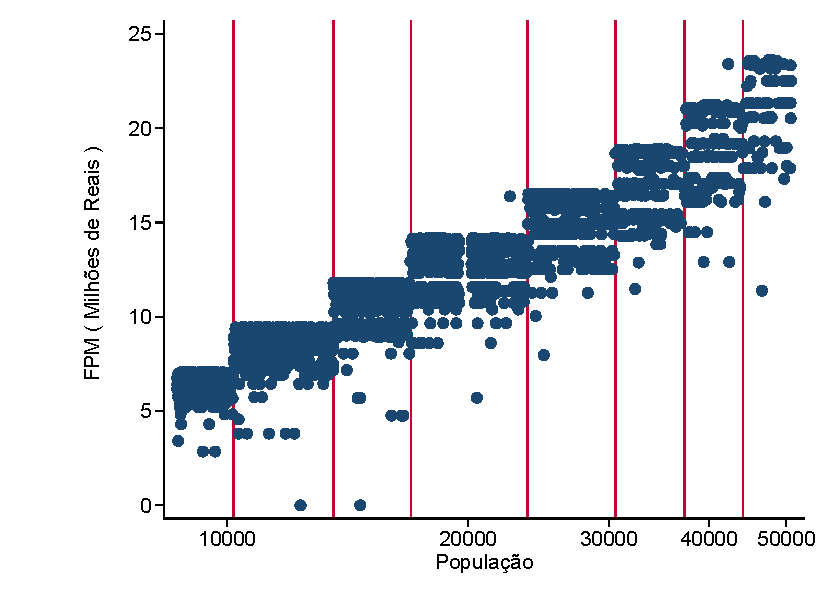
\includegraphics[scale=1.0]{Fpm.pdf}
    \end{center}
    \begin{flushleft}
    \vspace{-0.7cm}
     \caption*{Fonte: Elaboração própria, com base nos dados do IBGE. \\
    Nota: As linhas em vermelho representam os limiares populacionais especificados na tabela \ref{tab02}}
    \end{flushleft}
    \label{fig05}
\end{grafico}

Grande parte das despesas públicas dos municípios brasileiros é composta pelos gastos com pessoal, educação e saúde. De acordo com \citeonline{sen2010pessoas}, investir mais em saúde e educação tem efeitos positivos para o crescimento econômico nacional. Dessa forma, analisando o gasto nominal municipal com pessoal, é possível afirmar que, entre 1997 e 2017, os gastos com pessoal cresceram consideravelmente, principalmente entre 2010 e 2017, quanto a curva se tornou mais acentuada.

\begin{grafico}[H]
    \caption{Evolução do gasto com pessoal nos municípios brasileiros (1997 - 2017)}
    \vspace{-0.5cm}
    \begin{center}
    \includegraphics{Pessoal2.png}
    \end{center}
    \begin{flushleft}
    \vspace{-0.2cm}
    \hspace{1.6cm}
    Fonte: Elaboração própria com base nos dados do STN
    \end{flushleft}
    \label{fig06}
\end{grafico}


A Constituição Federal de 1988 define que certos bens ou serviços devem ser fornecidos para todos, isto é, devem ser universalizados. Desses bens, a educação e a saúde se destacam por ser bens básicos com grandes impactos de longo prazo. No caso do sistema educacional,  a legislação promoveu e dividiu em ensino de educação básica e superior. A educação básica, por sua vez, divide-se em três níveis: educação infantil (que compreende a faixa de 0 a 5 anos de idade), ensino fundamental, (de 6 a 14 anos de idade) e ensino médio, (de 15 a 17 anos de idade) ficando, a educação infantil e o ensino fundamental sob a responsabilidade dos municípios, enquanto o ensino médio fica, prioritariamente, sob a responsabilidade dos estados e do Distrito Federal. Cabe ao Governo Federal, dentre outras atribuições, atuar no ensino superior e prestar assistência técnica e financeira às esferas estadual e municipal, buscando garantir a equidade dos gastos nas diferentes Unidades da Federação.

Após as definições de competências, as políticas púbicas foram aprofundadas com a criação do Fundo de Manutenção e Desenvolvimento do Ensino Fundamental e de Valorização do Magistério (FUNDEF), instituído pela Lei no 9.424/1996, o qual vigorou até 2006 havendo depois sua ampliação, com o Fundo de Manutenção e Desenvolvimento da Educação Básica e de Valorização dos Profissionais da Educação (FUNDEB), institucionalizado pela Lei no 11.494/2007, que passou a destinar recursos para a educação básica, tanto na modalidade regular quanto na integrada à educação profissional e educação de jovens e adultos. No mesmo ano foi lançado o Plano de Desenvolvimento da Educação (PDE), que deu clara ênfase ao ensino fundamental e definiu metas para a melhoria da qualidade a partir do Índice de Desenvolvimento da Educação Básica - IDEB.

Também, merece destaque a Emenda Constitucional no 59/2009, que amplia a obrigatoriedade da educação básica para a faixa de 4 a 17 anos de idade que deveria ser implementada progressivamente até 2016. A Lei no 12.796/2013 oficializa essa mudança, alterando o texto original da Lei de Diretrizes e Bases da Educação (LDB), instituída pela Lei no 9.394/1996.  Com isso, a educação básica passa a ser obrigatória dos 4 aos 17 anos de idade e organizada em três etapas: pré-escola (nível obrigatório da educação infantil), ensino fundamental e ensino médio. 

Somado a esses avanços nas políticas educacionais, foi aprovado o Plano Nacional de Educação (PNE), de acordo com a Lei n. 13.005/2014, cujas 20 metas nacionais têm vigência por 10 anos. A Emenda Constitucional n. 59/2009, fez com que o PNE se tornasse uma exigência constitucional com periodicidade decenal, o que significa que planos plurianuais devem tomá-lo como referência. Assim, o PNE passou a ser considerado o articulador do Sistema Nacional de Educação (SNE), servindo de base para a elaboração dos planos estaduais, distrital e municipais, com previsão de percentual do Produto Interno Bruto - PIB para o seu financiamento.

Em relação a saúde, a Constituição Federal de 1988 estabeleceu um sistema descentralizado, onde os municípios são obrigados a prestar cuidados primários a seus residentes. A maioria dos gastos com saúde são executadas por governos subnacionais no Brasil, mas existe um fundo nacional unificado que tenta equalizar as discrepâncias nacionais: o Sistema Único de Saúde (SUS). Atualmente, mais de 70\% da população brasileira depende exclusivamente do SUS para atendimento médico e hospitalar, representando aproximadamente 150 milhões de cidadãos.

Nos últimos 20 anos, novas regras foram criadas para a regionalização dos serviços públicos, como a prestação de saúde nas Regiões de Saúde - RS (Decreto nº. 7.508/2011), formada pelo agrupamento de municípios vizinhos, seguindo a ideia de que a prestação de serviços de saúde devem ser integrados e coordenados nessas regiões. A grande virtude dessa agregação se da pelo acesso aos cuidados primários dos pacientes, que geralmente são feitos pelo atendimento ambulatorial e de emergência dos postos de saúde. Além disso, se a doença piorar, o paciente pode ser encaminhado para hospitais regionais, geralmente localizados nos maiores municípios das regiões de saúde.

A organização da rede de saúde pública justifica nossa amostra de cidades limítrofes. Quando uma cidade pequena contrata mais médicos, pode evitar o agravamento de doenças e, consequentemente, pode reduzir a demanda por hospitalização nas grandes cidades vizinhas. Os municípios também podem usar seus próprios recursos para financiar o sistema de saúde, incluindo subsídios incondicionais do Governo Federal, além das transferências condicionais do SUS \footnote{ As doações condicionais e obrigatórias têm um destino específico, enquanto as doações incondicionais, por sua vez, não têm um destino pré-estabelecido. O FPM é considerado uma concessão incondicional, uma vez que cada município tem a prerrogativa de gastar esse dinheiro onde há uma necessidade maior, uma característica que exploramos neste artigo.}.

Analisando os gastos por função dos principais setores de provisão do município (juntos representam, em média, 80\% da despesa pública municipal), percebe-se que, o gasto nas três funções (educação, saúde e administração) eram muito próximas no final dos anos 1990, sendo que até 1997, o gasto com administração era maior que os demais. Ao longo do tempo, os cortes com educação e saúde foram crescendo em proporções maiores que os alocados na função administrativa de forma que, logo depois de 2010, os gastos com as função educacional começaram a crescer em proporções maiores que os da saúde.

% Ajeitar essa figura, creio que aumentar kkkk

\begin{grafico}[H]
    \caption{Gastos dos municípios brasileiros, por função (1997-2017)}
    \vspace{-0.5cm}
    \begin{center}
    \includegraphics[scale=0.8]{Funcao.png}
    \end{center}
    \begin{flushleft}
        \vspace{-0.4cm}
        \hspace{1.3cm}
    Fonte: Elaboração própria com base nos dados do STN
        \end{flushleft}
        \label{fig07}
\end{grafico}

A Figura \ref{threshold}, abaixo, representa espacialmente os municípios que estão do lado esquerdo e direito dos três primeiros \textit{tresholds} do FPM em uma largura de 10\% em 2016. Percebe-se que espacialmente os municípios estão espalhados em todas as regiões brasileiras e que em alguns casos os municípios que estão a esquerda e a direita se apresentam próximos um dos outros. Nota-se também que os municípios pequenos estão concentradas no nordeste e sudeste, em regiões mais próximas ao litoral. No caso de Pará, Goiás e Rio Grande do Sul (estados com maiores números de municípios do Norte, Centro-Oeste e Sul, respectivamente) não apresentam muitos municípios quando se observa o caso de São Paulo, Rio de Janeiro, Minas Gerais e todos os estados do litoral nordestino.

Além disso, mesmo que de forma geral observa-se que os casos apresentam municípios do lado direito e esquerdo próximos, a região do sudeste apresenta mais casos de municípios pequenos do lado esquerdo do FPM, enquanto que o nordeste apresenta maiores municípios pequenos do lado direito do FPM.

\begin{figure}[H]
    \centering
    \caption{Municípios ao longo do três primeiros tresholds (2016)}
    \includegraphics[scale=0.8]{threshold.png}
    \vspace{-1cm}
    \label{threshold}
\end{figure}

O Brasil, por ser um país muito grande, há dificuldades de analisar e controlar as políticas administrativas dos municípios locais. Em muitos casos os municípios pequenos não desenvolvem uma boa gestão, em algumas ocasiões a sua receita própria não consegue sustentar o gasto com a prefeitura. Com outras palavras, o município não possui nenhuma condição de se sustentar. É necessário que exista equilíbrio nas contas públicas para que seja garantida um ambiente competitivo no quesito de geração de emprego e renda para a população.

Desta forma, com o objetivo de contribuir com o debate sobre a eficiência da gestão fiscal, tendo como foco a administração dos recursos públicos buscando analisar a qualidade do gasto público municipal, o sistema FIRJAN criou um indicador que busca mensurar a qualidade da gestão fiscal dos municípios: O Índice FIRJAN de Gestão Fiscal. 

A metodologia do IFGF é composta por por quatro indicadores – Autonomia, Gastos com Pessoal, Liquidez e Investimentos. A leitura de seus resultados é bastante simples: a pontuação varia entre 0 e 1, sendo que os municípios com as melhores gestões estão próximas de 1. De 0 a 0.4 possuem qualidade de gestão crítica, de 0.41 até 0.6 possuem qualidade de gestão com dificuldade de administração, de 0.61 ate 0.8 possui uma boa qualidade de gestão e 0.81 até 1 são os municípios com qualidade e gestão administrativa excelente.

A pontuação que os municípios recebem depende da avaliação dos quatro indicadores:

\begin{itemize}
    \item Receita Própria : Mede a "capacidade de arrecadação de cada município e sua dependência das transferências de recursos dos governos estadual e federal".
    \item Gastos com Pessoal : Representa o "gasto dos municípios com o quadro de servidores, avaliando o grau de rigidez do orçamento para execução das políticas públicas".
    \item Liquidez : Verifica a “relação entre o total de restos a pagar acumulados no ano e os ativos financeiros disponíveis para pagá-los no exercício seguinte”.
    \item Investimentos : Acompanha o "total de investimentos em relação à receita líquida".
\end{itemize}

Os quatro representam 25\% sobre o resultado final. Com os números em mãos é possível saber, por exemplo, em quais municípios o gasto com pessoal ultrapassou o limite de 60\% das receitas estabelecido pela Lei de Responsabilidade Fiscal. Ou, ainda, saber se a prefeitura faz investimentos públicos para melhorias para o cidadão de seu município.

Por exemplo, em 2018, se destacam a falta de condições de financiar a estrutura administrativa com recursos da economia local, a elevada rigidez do orçamento das prefeituras, sobretudo, com gastos com pessoal e as dificuldades de cumprir as obrigações financeiras e de gerar bem-estar e competitividade por meio de investimentos.

O indicador se mostra pertinente para análise, uma vez que sua abrangência geográfica cobre o desempenho econômico de cerca de 5.337 cidades brasileiras. Além disso, o indicador tem resultados a partir de 2006 até 2018.

A conclusão dos resultados de 2018 é que 73,9\% desses municípios estão em situação fiscal difícil ou crítica. Das 5.337, 3.944 cidades estão nesta condição, incluindo nove capitais: Florianópolis, Maceió, Porto Velho, Belém, Campo Grande, Natal, Cuiabá, Rio de Janeiro e São Luís.

Todos os municípios que foram analisados, declararam suas contas à Secretaria do Tesouro Nacional (STN). Outros 231 municípios ficaram de fora porque não informaram os dados no prazo ou havia alguma inconsistência na declaração. O fato dessa fração ser pequena em relação ao total demonstra um avanço na transparência das informações.

Por ser um índice com abrangência nacional e comparação anual, o IFGF assume mais de uma função: 

\begin{itemize}
    \item Mapa dos principais entraves em torno do Pacto Federativo
    \item Instrumento de suporte para gestores públicos de todo o país administrarem suas contas de forma eficiente
    \item Ferramenta de controle social para os cidadãos sobre a administração dos recursos públicos
    \item \textit{Rating} para investidores sobre ambiente de negócios
\end{itemize}

Os dados são construídos com base em resultados fiscais oficiais que são declarados pelas próprias prefeituras. Conforme estabelecido pelo Artigo 51 da Lei de Responsabilidade Fiscal (2000), os municípios são obrigados a declarar suas contas para a Secretaria do Tesouro Nacional (STN) até o dia 30 de abril do ano seguinte ao exercício de referência. Dessa forma, a STN dispõe de 60 dias para disponibilizá-las ao público, por meio do Sistema de Informações Contábeis e Fiscais do Setor Público Brasileiro (Siconfi\footnote{ O Siconfi é a principal fonte de dados relacionadas as administrações públicas municipais e estaduais. Por isso, o IFGF utiliza essa base para calculo do indicador.}).

O IFGF Autonomia se torna um dos indicadores mais importantes a ser analisado por evidenciar a baixa capacidade de sustentabilidade do município. A Constituição Federal de 1988, apesar de ter muitos pontos positivos, com a proposta de descentralização da administração pública permitiu a flexibilização na emancipação de municípios. Apesar do crescimento ser expressivo, a magnitude não é um problema, desde que os municípios consigam aplicar na prática o propósito de sua emancipação, que é gerar mais bem estar para a população. Dessa forma, o IFGF Autonomia busca analisar em seu calculo se as prefeituras brasileiras possuem recursos suficientes para arcar com seus custos de existência, caso contrário, o principal objetivo de emancipação de uma prefeitura pode estar ameaçado.

Em relação ao gasto com pessoal, \citeonline{velloso2006ajuste} lembra que o gasto com pessoal é uma despesa fixada por lei ao pagamento de salários e aposentadorias de servidores. O aumento desses gastos implica na redução dos recursos destinadas as outras áreas, afetando as políticas públicas. A Lei de Responsabilidade Fiscal (LRF) limita os gastos com pessoal em até 60\% da Receita Corrente Líquida (RCL) para que não seja utilizado desse gasto em excesso. Por isso, o IFGF Gastos com Pessoal busca analisar se os gastos com pessoas dos municípios estão comprometendo suas respectivas receitas.

Já quando se fala em restos a pagar, consideramos que esta questão se destina a compatibilizar o exercício financeiro com a continuidade da administração pública, uma vez que há a possibilidade de existir pagamentos pendentes de gestões anteriores que foram postergadas. \citeonline{nascimento2002lei} ressaltam que ao longo do tempo, restos a pagar se tornou uma simples postergação de despesas já contratadas para outros anos, gerando um problema de liquidez para as gestões dos municípios.

A LRF estabeleceu então que no último ano de mandato, os governos subnacionais possuam recursos financeiros suficientes para arcar com as despesas que foram postergadas para o ano seguinte. Dessa forma, no cálculo do índice do IFGF Liquidez, caso o município tenha declarado mais restos a pagar do que recursos em Caixa no ano da inscrição de suas informações, sua pontuação será zero. Na interpretação de seus resultados, quanto mais próximo de 1, menos o município está postergando pagamentos para o exercício seguinte sem a devida cobertura. Mesmo que a LRF só destaque os últimos anos de gestão, esse indicador busca também analisar o quanto o município posterga suas dividas.

Por fim, temos o IFGF investimento, que tem o objetivo medir a parcela dos investimentos nos orçamentos municipais. Por mais que haja consenso literário sobre como é importante que o município realize investimentos na área principais, como saúde e educação para que haja crescimento econômico e diminuição das desigualdades sociais, sabemos também que o processo orçamentário é “míope” e atribui maiores importâncias a projetos que tragam benefícios a curto prazo \cite{gobetti2007indice}.

Por isso, o indicador estabelece que municípios que investiram mais que 12\% da sua receita total terão sua nota atribuída a 1 e o restante terá sua nota atribuída a quão próximo o município estará dessa nota de corte.

A figura \ref{ifgf.fig} representado abaixo pelo mapa mostra que os municípios que apresentaram menores notas no IFGF são os municípios situados no Norte e Nordeste, enquanto que os resultados bons estão situados nas regiões sul, sudeste e centro oeste. Por fim, os municípios com nota excelente ficaram situados na região centro oeste do Brasil.

Olhando de forma específica, o FIRJAN afirma que cerca de 1.856 municípios não se sustentam porque sua receita própria não é suficiente para pagar seus próprios gastos com a estrutura administrativa. Dentre os indicadores, o que puxou mais os resultados para baixo foi o de Autonomia, demonstrando que muitos municípios não possuem condições de se sustentar. De acordo ainda com o FIRJAN, para que as contas fossem equilibradas os municípios precisariam aumentar suas receitas próprias em 50\%. Contudo, a entidade acredita improvável, uma vez que os mesmos só tiveram um aumento real de apenas 9,6\% nos últimos 5 anos.

No Nordeste 71\% e no Norte 45,6\% das prefeituras não possuem condições de se sustentar, ou seja, ficaram com nota zero no quesito. Na região Sul, 6,6\% dos municípios receberam zero no indicador, no Centro-Oeste 16,4\% e 18,6\% no Sudeste. A entidade afirma que a baixa geração de receita dentro do município explica disparidades regionais: No Nordeste e no Norte a receita local líquida por pessoa é um terço da gerada nas outras regiões. A menor é no Nordeste (R\$ 298) enquanto a mais elevada é no Sul (R\$1.294).

\begin{figure}[H]
    \centering
    \caption{Resultados do Índice Firjan (2016)}
    \includegraphics[scale=0.8]{ifgf.png}
    \label{ifgf.fig}
\end{figure}

\section{Resultados Empíricos}

As seções anteriores fizeram um breve apanhado da literatura relacionando o FPM como instrumento de análise empírica. Em seguida foi apresentado o método da Regressão Descontinua, bem como sua construção algébrica e os pressupostos do modelo. Por último, foi feita uma breve análise sobre os resultados históricos das finanças públicas do Brasil. As informações obtidas abrem espaço para maiores discussões, uma vez que a literatura não aprofunda a parte qualitativa do gasto e existe base de dados disponíveis.

% Nos últimos anos o Estado vem apresentando dificuldades financeiras em todas as esferas governamentais. Por isso, para municípios pequenos se torna muito importante qualquer ganho de receita e a forma como ele administra seus recursos viram debate a ser discutido. A questão da economicidade já é discutida desde a Constituição de 1988, que trata da necessidade do desenvolvimento de indicadores para a avaliação dos resultados das políticas públicas e dos respectivos gastos públicos, nas áreas de Educação, Saúde, Transportes, Habitação, Meio Ambiente, etc.

Por isso, o objetivo desta seção é analisar o impacto dos ganhos de transferência no comportamento orçamentário municipal, considerando o desenvolvimento de abordagens baseadas em incentivos para apoiar a melhoria da prestação de serviços locais, além do método aplicado que também oferece uma estrutura simples, consistente e abrangente para avaliar empiricamente a existência e impacto de incentivos perversos.

Mas antes, é necessário analisar a existência de uma possível manipulação dos resultados populacionais. O teste \citeonline{mccrary2008manipulation} tem como objetivo garantir a hipótese básica para a análise do RDD, uma vez que a existência de manipulação do experimento torna os resultados viesados, por isso, inconclusivo. A tabela \ref{manipulacao} abaixo, apresenta os resultados obtidos do teste. O p-valor maior que 10\% em todas as faixas e bandas de larguras rejeitam a hipótese de manipulação e indicam que as estimativas populacionais não apresentam sinais de manipulação dos resultados para nenhuma das bandas de larguras escolhidas para a análise \footnote{Os resultados gráficos são apresentados no apêndice por Figura \ref{mccrary1}, \ref{mccrary2} e \ref{mccrary3}}. 

Este resultado é diferente do encontrado por \citeonline{monasterio2013fpm}, que retrata a capacidade dos municípios de manipular as estimativas populacionais.  \citeonline{araujomatos2019} argumentam que os resultados das estimativas populacionais não apresentam evidências de manipulação populacional por ser um resultado diluído do Censo Demográfico (que possuiu evidências de manipulação). A tendência, então, é que as estimativas populacionais corrijam o viés do Censo.

% Table generated by Excel2LaTeX from sheet 'Planilha2'
\begin{table}[H]
  \centering
  \caption{Resultado do teste de manipulação para população}
    \begin{tabular}{llllll}
    \toprule
    \multicolumn{1}{l|}{Faixas Populacionais} & \multicolumn{1}{c}{2\%} & \multicolumn{1}{c}{3\%} & \multicolumn{1}{c}{4\%} & \multicolumn{1}{c}{10\%} & \multicolumn{1}{c}{15\%} \\
    \midrule
    \multicolumn{1}{l|}{1º Faixa (10,188)} & \multicolumn{1}{r}{-1.4643} & \multicolumn{1}{r}{-1.4367} & \multicolumn{1}{r}{-0.9062} & \multicolumn{1}{r}{-1.071} & \multicolumn{1}{r}{-0.5797} \\
    \multicolumn{1}{l|}{Prob} & \multicolumn{1}{r}{0.1431} & \multicolumn{1}{r}{0.1508} & \multicolumn{1}{r}{0.3648} & \multicolumn{1}{r}{0.2842} & \multicolumn{1}{r}{0.5621} \\
    \midrule
    \multicolumn{1}{l|}{2º Faixa (13,584)} & \multicolumn{1}{r}{0.5903} & \multicolumn{1}{r}{0.5283} & \multicolumn{1}{r}{-0.2935} & \multicolumn{1}{r}{-0.3019} & \multicolumn{1}{r}{-0.7815} \\
    \multicolumn{1}{l|}{Prob} & \multicolumn{1}{r}{0.555} & \multicolumn{1}{r}{0.5973} & \multicolumn{1}{r}{0.7691} & \multicolumn{1}{r}{0.7628} & \multicolumn{1}{r}{0.4345} \\
    \midrule
    \multicolumn{1}{l|}{3º Faixa (16,980)} & \multicolumn{1}{r}{0.959} & \multicolumn{1}{r}{0.6227} & \multicolumn{1}{r}{-0.3091} & \multicolumn{1}{r}{-0.1085} & \multicolumn{1}{r}{-0.3504} \\
    \multicolumn{1}{l|}{Prob} & \multicolumn{1}{r}{0.3375} & \multicolumn{1}{r}{0.5335} & \multicolumn{1}{r}{0.7573} & \multicolumn{1}{r}{0.9136} & \multicolumn{1}{r}{0.726} \\
    \midrule
    \multicolumn{6}{l}{Fonte: Elaboração própria} \\
    \end{tabular}%
  \label{manipulacao}%
\end{table}%

Com a rejeição de manipulação e definidas as variáveis que serão utilizadas, a tabela \ref{tab:est}, apresenta a estatística descritiva dessas variáveis de interesse e das co-variadas. A primeira coluna representa os municípios com menos de 44148 habitantes residentes (municípios pequenos). As demais colunas explicitam os resultados para os municípios com populações entre 8500 e 18700 habitantes (situadas nas três primeiras faixas do FPM) separadas por nível agregado do Brasil e em Grandes Regiões.

Ao avaliar os resultados médios de cada variável de interesse, constata-se que, a receita e despesa em proporção do PIB são maiores nos municípios do estado do Nordeste e Sudeste. Pela Figura \ref{fig04}, é possível observar que a maioria dos municípios sob o intervalo populacional de interesse se encontram na região Nordeste. Por se tratar muitas vezes de municípios mais pobres, a razão da receita e despesa em função do PIB é alto devido a esses municípios terem o PIB pequeno.

Os resultados também mostram que, o Nordeste apresenta a maior proporção de receita oriunda do FPM e é a segunda região que menos tem proporção de receita própria (perdendo apenas para o norte, que possui o maior número de participação em outras transferências). Esses resultados nos mostram que os municípios do Nordeste são mais dependentes que os demais por necessitar mais do FPM. Em alguns situações, caso não houvesse a transferência, o município não teria condições de liquidar as suas despesas.

Já para os gastos, observa-se que o Nordeste também aparece como a região que tem a maior participação dos gastos médios em educação. O Sudeste, por sua vez, tem maior proporção de gasto médio em saúde e o Norte com os gastos com administrativo. Em outras palavras, essas regiões possuem o maior foco das despesas de seus orçamentos nas respectivas funções.

De forma geral, estes resultados prévios também mostram que a receita própria possui baixa participação na receita total, mostrando que em média os municípios são bastantes dependentes das transferências. Do lado da despesa, os três maiores gastos se encontram na esfera educacional, saúde e administrativo (por ordem) e esses gastos são, na maior parte, destinados a gastos com pessoal.

% Table generated by Excel2LaTeX from sheet 'Plan1'
\begin{table}[H]
  \centering
  \caption{Estatística Descritiva das variáveis utilizadas}
    \begin{tabular}{llllllll}
    \toprule
    \multicolumn{1}{c|}{\multirow{3}[6]{*}{Variáveis}} & \multicolumn{7}{c}{Faixa populacional} \\
\cmidrule{2-8}    \multicolumn{1}{c|}{} & \multicolumn{1}{l|}{7500-44148} & \multicolumn{6}{c}{8500 - 18700} \\
\cmidrule{2-8}    \multicolumn{1}{c|}{} & \multicolumn{1}{c|}{Total} & \multicolumn{1}{c}{Total} & \multicolumn{1}{c}{Norte} & \multicolumn{1}{c}{Nordeste} & \multicolumn{1}{c}{Sudeste} & \multicolumn{1}{c}{Sul} & \multicolumn{1}{c}{CO} \\
    \midrule
    \multicolumn{8}{l}{\textbf{Receita}} \\
    \midrule
    \multicolumn{1}{l|}{Receita/PIB} & \multicolumn{1}{c|}{17,003} & \multicolumn{1}{c}{18,514} & \multicolumn{1}{c}{14,661} & \multicolumn{1}{c}{26,573} & \multicolumn{1}{c}{14,772} & \multicolumn{1}{c}{10,176} & \multicolumn{1}{c}{11,463} \\
    \midrule
    \multicolumn{1}{l|}{\% FPM} & \multicolumn{1}{c|}{0.30} & \multicolumn{1}{c}{0.32} & \multicolumn{1}{c}{0.27} & \multicolumn{1}{c}{0.37} & \multicolumn{1}{c}{0.32} & \multicolumn{1}{c}{0.27} & \multicolumn{1}{c}{0.26} \\
    \multicolumn{1}{l|}{\% Outras Transf} & \multicolumn{1}{c|}{0.32} & \multicolumn{1}{c}{0.30} & \multicolumn{1}{c}{0.36} & \multicolumn{1}{c}{0.29} & \multicolumn{1}{c}{0.29} & \multicolumn{1}{c}{0.29} & \multicolumn{1}{c}{0.33} \\
    \multicolumn{1}{l|}{\% Receita Própria} & \multicolumn{1}{c|}{0.06} & \multicolumn{1}{c}{0.05} & \multicolumn{1}{c}{0.04} & \multicolumn{1}{c}{0.03} & \multicolumn{1}{c}{0.06} & \multicolumn{1}{c}{0.08} & \multicolumn{1}{c}{0.09} \\
    \multicolumn{1}{l|}{\% Transf Estadual} & \multicolumn{1}{c|}{0.19} & \multicolumn{1}{c}{0.19} & \multicolumn{1}{c}{0.20} & \multicolumn{1}{c}{0.10} & \multicolumn{1}{c}{0.24} & \multicolumn{1}{c}{0.26} & \multicolumn{1}{c}{0.26} \\
    \midrule
    \multicolumn{8}{l}{\textbf{Despesa}} \\
    \midrule
    \multicolumn{1}{l|}{Despesa/PIB} & \multicolumn{1}{c|}{15,510} & \multicolumn{1}{c}{16,868} & \multicolumn{1}{c}{13,413} & \multicolumn{1}{c}{24,722} & \multicolumn{1}{c}{13,142} & \multicolumn{1}{c}{8,772} & \multicolumn{1}{c}{9,888} \\
    \midrule
    \multicolumn{1}{l|}{\% Pessoal} & \multicolumn{1}{c|}{0.53} & \multicolumn{1}{c}{0.53} & \multicolumn{1}{c}{0.52} & \multicolumn{1}{c}{0.55} & \multicolumn{1}{c}{0.51} & \multicolumn{1}{c}{0.49} & \multicolumn{1}{c}{0.51} \\
    \multicolumn{1}{l|}{\% Capital} & \multicolumn{1}{c|}{0.10} & \multicolumn{1}{c}{0.10} & \multicolumn{1}{c}{0.12} & \multicolumn{1}{c}{0.09} & \multicolumn{1}{c}{0.10} & \multicolumn{1}{c}{0.12} & \multicolumn{1}{c}{0.09} \\
    \midrule
    \multicolumn{1}{l|}{\% Educação} & \multicolumn{1}{c|}{0.34} & \multicolumn{1}{c}{0.34} & \multicolumn{1}{c}{0.38} & \multicolumn{1}{c}{0.40} & \multicolumn{1}{c}{0.28} & \multicolumn{1}{c}{0.27} & \multicolumn{1}{c}{0.28} \\
    \multicolumn{1}{l|}{\% Saúde} & \multicolumn{1}{c|}{0.23} & \multicolumn{1}{c}{0.23} & \multicolumn{1}{c}{0.20} & \multicolumn{1}{c}{0.22} & \multicolumn{1}{c}{0.26} & \multicolumn{1}{c}{0.24} & \multicolumn{1}{c}{0.24} \\
    \multicolumn{1}{l|}{\% Administração} & \multicolumn{1}{c|}{0.14} & \multicolumn{1}{c}{0.14} & \multicolumn{1}{c}{0.17} & \multicolumn{1}{c}{0.14} & \multicolumn{1}{c}{0.14} & \multicolumn{1}{c}{0.14} & \multicolumn{1}{c}{0.16} \\
    \multicolumn{1}{l|}{\% Agricultura} & \multicolumn{1}{c|}{0.01} & \multicolumn{1}{c}{0.02} & \multicolumn{1}{c}{0.02} & \multicolumn{1}{c}{0.01} & \multicolumn{1}{c}{0.01} & \multicolumn{1}{c}{0.03} & \multicolumn{1}{c}{0.01} \\
    \multicolumn{1}{l|}{\% Desporto e Lazer} & \multicolumn{1}{c|}{0.01} & \multicolumn{1}{c}{0.01} & \multicolumn{1}{c}{0.01} & \multicolumn{1}{c}{0.01} & \multicolumn{1}{c}{0.01} & \multicolumn{1}{c}{0.01} & \multicolumn{1}{c}{0.01} \\
    \multicolumn{1}{l|}{\% Encargos Especiais} & \multicolumn{1}{c|}{0.02} & \multicolumn{1}{c}{0.02} & \multicolumn{1}{c}{0.01} & \multicolumn{1}{c}{0.01} & \multicolumn{1}{c}{0.02} & \multicolumn{1}{c}{0.03} & \multicolumn{1}{c}{0.01} \\
    \multicolumn{1}{l|}{\% Legislativo} & \multicolumn{1}{c|}{0.03} & \multicolumn{1}{c}{0.03} & \multicolumn{1}{c}{0.03} & \multicolumn{1}{c}{0.03} & \multicolumn{1}{c}{0.03} & \multicolumn{1}{c}{0.02} & \multicolumn{1}{c}{0.04} \\
    \multicolumn{1}{l|}{\% Previdência} & \multicolumn{1}{c|}{0.02} & \multicolumn{1}{c}{0.02} & \multicolumn{1}{c}{0.01} & \multicolumn{1}{c}{0.01} & \multicolumn{1}{c}{0.03} & \multicolumn{1}{c}{0.02} & \multicolumn{1}{c}{0.04} \\
    \multicolumn{1}{l|}{\% Transporte} & \multicolumn{1}{c|}{0.02} & \multicolumn{1}{c}{0.02} & \multicolumn{1}{c}{0.03} & \multicolumn{1}{c}{0.01} & \multicolumn{1}{c}{0.02} & \multicolumn{1}{c}{0.06} & \multicolumn{1}{c}{0.04} \\
    \midrule
    \multicolumn{8}{l}{\textbf{Controle}} \\
    \midrule
    \multicolumn{1}{l|}{Empresas} & \multicolumn{1}{c|}{617} & \multicolumn{1}{c}{417} & \multicolumn{1}{c}{192} & \multicolumn{1}{c}{184} & \multicolumn{1}{c}{620} & \multicolumn{1}{c}{706} & \multicolumn{1}{c}{532} \\
    \multicolumn{1}{l|}{Empregados} & \multicolumn{1}{c|}{2,465} & \multicolumn{1}{c}{1,575} & \multicolumn{1}{c}{931} & \multicolumn{1}{c}{873} & \multicolumn{1}{c}{2,055} & \multicolumn{1}{c}{2,582} & \multicolumn{1}{c}{2,039} \\
    \multicolumn{1}{l|}{PIB (mil)} & \multicolumn{1}{c|}{4,026} & \multicolumn{1}{c}{2,548} & \multicolumn{1}{c}{2,066} & \multicolumn{1}{c}{1,323} & \multicolumn{1}{c}{3,170} & \multicolumn{1}{c}{4,030} & \multicolumn{1}{c}{4,100} \\
    \multicolumn{1}{l|}{IFDM} & \multicolumn{1}{c|}{0.64} & \multicolumn{1}{c}{0.64} & \multicolumn{1}{c}{0.55} & \multicolumn{1}{c}{0.57} & \multicolumn{1}{c}{0.7} & \multicolumn{1}{c}{0.73} & \multicolumn{1}{c}{0.67} \\
    \multicolumn{1}{l|}{IFGF} & \multicolumn{1}{c|}{0.44} & \multicolumn{1}{c}{0.44} & \multicolumn{1}{c}{0.41} & \multicolumn{1}{c}{0.31} & \multicolumn{1}{c}{0.48} & \multicolumn{1}{c}{0.62} & \multicolumn{1}{c}{0.54} \\
    \multicolumn{1}{l|}{IFGF Autonomia} & \multicolumn{1}{c|}{0.38} & \multicolumn{1}{c}{0.35} & \multicolumn{1}{c}{0.20} & \multicolumn{1}{c}{0.05} & \multicolumn{1}{c}{0.50} & \multicolumn{1}{c}{0.73} & \multicolumn{1}{c}{0.58} \\
    \multicolumn{1}{l|}{IFGF Investimento} & \multicolumn{1}{c|}{0.51} & \multicolumn{1}{c}{0.53} & \multicolumn{1}{c}{0.60} & \multicolumn{1}{c}{0.51} & \multicolumn{1}{c}{0.51} & \multicolumn{1}{c}{0.62} & \multicolumn{1}{c}{0.49} \\
    \multicolumn{1}{l|}{IFGF Liquidez} & \multicolumn{1}{c|}{0.47} & \multicolumn{1}{c}{0.47} & \multicolumn{1}{c}{0.47} & \multicolumn{1}{c}{0.40} & \multicolumn{1}{c}{0.46} & \multicolumn{1}{c}{0.57} & \multicolumn{1}{c}{0.67} \\
    \multicolumn{1}{l|}{IFGF Pessoal} & \multicolumn{1}{c|}{0.39} & \multicolumn{1}{c}{0.4} & \multicolumn{1}{c}{0.38} & \multicolumn{1}{c}{0.29} & \multicolumn{1}{c}{0.46} & \multicolumn{1}{c}{0.57} & \multicolumn{1}{c}{0.43} \\
    \multicolumn{1}{l|}{Possibilidade de Reeleição} & \multicolumn{1}{c|}{0.80} & \multicolumn{1}{c}{0.79} & \multicolumn{1}{c}{0.80} & \multicolumn{1}{c}{0.78} & \multicolumn{1}{c}{0.82} & \multicolumn{1}{c}{0.75} & \multicolumn{1}{c}{0.88} \\
    \multicolumn{1}{l|}{Experiência Gestão} & \multicolumn{1}{c|}{0.20} & \multicolumn{1}{c}{0.20} & \multicolumn{1}{c}{0.19} & \multicolumn{1}{c}{0.22} & \multicolumn{1}{c}{0.18} & \multicolumn{1}{c}{0.24} & \multicolumn{1}{c}{0.12} \\
    \midrule
    \multicolumn{8}{l}{Fonte: Elaboração própria} \\
    \end{tabular}%
  \label{tab:est}%
\end{table}%

Contudo, esses resultados ainda são inconclusivos. Como não estamos lidando com um experimento aleatório, a análise de diferença de médias é viesado devido ao erro de seleção, sendo necessário adotar um método mais robusto para a análise de impacto das transferências. Por isso, opta-se por estimar de forma linear pelo método \textit{Sharp} de Regressão Descontínua com as amostras abrangendo municípios situados ao redor dos três primeiros pontos de corte do FPM (10189, 13585 e 16981 habitantes); e utilizando um de \textit{threshold} de 4\%, 5\%, 10\% e 15\%. A definição dos cortes se limitou apenas as três primeiras devido ao enfraquecimento do impacto dos limiares com o crescimento do tamanho populacional municipal.

\subsection{Transferências}

A primeira etapa a ser feita é encontrar quais tipos de receitas podem apresentar descontinuidade. O que se espera é que, nenhuma outra transferência além do FPM gere a descontinuidade na mesma situação de limiar populacional. O resultado apresentado no gráfico \ref{graph1} mostra que o FPM se apresenta bastante significativo e evidência que a constituição gera descontinuidade nessas transferências. Os resultados também mostram que outras transferências e as transferências estaduais não apresentam descontinuidade. Por fim, mesmo que a receita própria apresente descontinuidade, ela acaba não sendo estatisticamente significativa, como vemos na Tabela \ref{tabela_receita}.

Pelo trabalho de \citeonline{regatieri2013tributos} ter gerado resultados mais robustos ao cobrir integralmente os anos da série 2000-2011 e faixas populacionais completas; dele se depreende que as pequenas cidades brasileiras não aumentam as receitas próprias em resposta a um incremento do FPM per capita. Por isso é possível afirmar que, o sentido da interação entre o FPM e as políticas de arrecadação dos municípios com base nos resultados obtidos são válidos. A indiferença comportamental também pode ser considerada um incentivo perverso, uma vez que tal política gere indiferença do município em procurar outros meios de arrecadação.

\begin{figure}[H]%
    \centering
    \caption{Descontinuidade nas receitas}%
    \vspace{-0.5cm}
    \includegraphics[width=15cm]{Graph1.pdf} %
    \begin{flushleft}
        \vspace{-0.4cm}
        \hspace{1.3cm}
    Fonte: Elaboração própria com base nos dados do IBGE e STN
    \end{flushleft}
    \label{graph1}%
\end{figure}

\subsection{Despesa Total}

A próxima etapa é investigar o efeito das transferências federais na despesa total dos municípios. É necessário saber como o FPM afeta a despesa total dos municípios próximos à faixa. O resultado do gráfico \ref{receita} mostra que a despesa apresenta significância estatística na descontinuidade. As regressões de robustez apresentada na tabela \ref{gasto_table} do apêndice reforçam o do gráfico, indicando que a descontinuidade do FPM implica em uma descontinuidade nos gastos totais dos municípios. Vale salientar que por se tratar da despesa total, os parâmetros não estão distantes da significância, mas perdem significância estatística devido a erros-padrão mais elevados.

Com a significância desta variável e confirmação do que já foi debatido pela literatura, a próxima etapa da análise é verificar em que tipo de função esse gasto gera descontinuidade e qual o possível canal de transmissão (se os gastos estão direcionados mais a pessoal ou capital).

% O resultado obtido também é o esperado pela literatura mostrando consistência com o que é encontrado por outros autores\footnote{Ver \citeonline{brollo2013political}, \citeonline{litschig2013impact}, \citeonline{araujomatos2019}}, apontando para um efeito grande e significativo dos lucros fiscais e nas despesas orçamentárias.


\begin{figure}[H]%
    \centering
    \caption{Descontinuidade da despesa e receita}%
    \includegraphics[width=16cm]{Graph2.pdf} %
    \begin{flushleft}
        \vspace{-0.4cm}
        \hspace{1.3cm}
    Fonte: Elaboração própria com base nos dados do IBGE e STN
    \end{flushleft}
    \label{receita}%
\end{figure}

As políticas públicas assumem um papel importante para a sociedade quando são pensadas de forma ordenada e de acordo com as demandas e interesses sociais no estímulo ao crescimento econômico, fomento ao desenvolvimento humano, a formação da cidadania e a redução de desigualdades sociais e regionais.

Como já foi relatado, no contexto brasileiro, a Constituição Federal de 1988 abriu as portas para a concretização de diversas políticas públicas no Brasil como, por exemplo, a implementação de programas de combate à fome e a pobreza, educação e saúde universalizados. Já a Lei de Responsabilidade Fiscal, em 2000, teve grande importância com a criação e estabelecimento de metas a serem atingidas por todos os entes federados.

\subsubsection{Despesa Orçamentária}

Podemos definir as despesas com pessoal como qualquer gasto realizado que seja direcionada a pagamento da folha salarial dos empregados do setor público. 

As despesas com capital são despesas cuja finalidade é o planejamento e execução de obras, aquisição de instalações, equipamentos, material permanente, constituição ou aumento do capital do Estado que não sejam de caráter comercial ou financeiro, incluindo as aquisições de imóveis considerados necessários à execução de tais obras. 

Dentro das despesas com capital também tem as inversões financeiras, que são despesas cuja finalidade é a aquisição de imóveis, bens de capital já em utilização, títulos representativos de capital de entidades já constituídas (desde que a operação não importe em aumento de capital), constituição ou aumento de capital de entidades comerciais ou financeiras (inclusive operações bancárias e de seguros). Em suma, são operações que importem a troca de dinheiro por bens.

Os resultado do gráfico \ref{rdd_funcao} mostra que a descontinuidade não apresenta significância estatística do gasto com capital. Mesmo que graficamente se observe descontinuidade, o intervalo de confiança é elevado, de forma que apenas em alguns casos sejam significantes e não tenha como afirmar que as transferências geram descontinuidade nesses gastos. Já os gastos com pessoal apresentam indícios de descontinuidade na trajetória linear, mas a descontinuidade parece ter pequena magnitude. Na tabela \ref{tabela_pessoal} do apêndice se torna possível confirmar os resultados, uma vez que se encontra significância estatística em todas as bandas de largura quando se agrega as faixas. Dessa forma, mesmo que não sejam fortes evidências, a descontinuidade do FPM impacta positivamente nas despesas totais, mais especificamente nos gastos com pessoal do município.

\begin{figure}[H]%
    \centering
    \caption{Descontinuidade dos gastos com pessoal e capital}%
    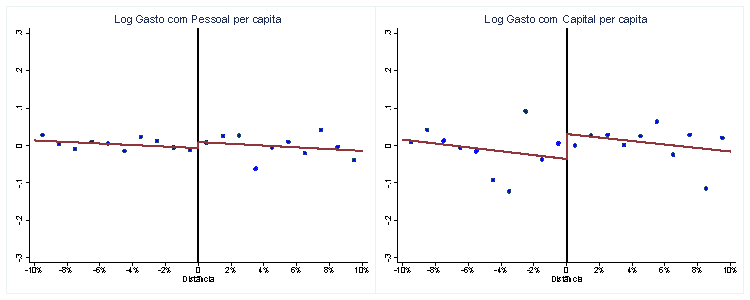
\includegraphics[width=15cm]{Graph6.pdf} %
    \begin{flushleft}
        \vspace{-0.4cm}
        \hspace{1.3cm}
    Fonte: Elaboração própria com base nos dados do IBGE e STN
    \end{flushleft}
    \label{rdd_funcao}%
\end{figure}

\subsubsection{Por função}

Com evidência de que o acréscimo de receita exógena causada pela estrutura constitucional do FPM gera descontinuidade nos gastos totais e de forma específica nos gastos com pessoal, a próxima etapa é encontrar qual comportamento na despesa por função esta tendo o município com o aumento de receita.

Existem dois pontos que tornam importante analisar esses comportamentos: o município que utiliza esses ganhos para aumentar suas despesas em áreas como em empregabilidade ou legislativo pode implicar em incentivos perversos. Por outro lado, municípios que gastam mais com Saúde, Educação, Segurança, Desportivo e Lazer e Transporte leva a crer que as transferências geram incentivos benéficos. A expectativa é que o incentivo das transferências siga os pressupostos da Teoria Normativa em que o país adquire pontos positivos com a descentralização.

Os resultados gerais apontam que os municípios apresentam incentivos em aumentar apenas seus gastos com a prefeitura municipal. Mesmo que em alguns casos como Saúde, Desportivo e Lazer e Legislativo apresentem alguma significância em alguns casos, não há como inferir sob este resultado. No gráfico \ref{funcao1} observa-se que o gasto com administrativo parece ser bastante significativa.

Os gastos com saúde e educação, que teoricamente seriam os recursos com impacto positivo no desenvolvimento local, não apresentaram significância estatística (no caso da educação não parece apresentar nenhum tipo de descontinuidade). Quando estes resultados são aplicadas em outras situações de robustez o resultado não muda: apenas os gastos com administrativos apresentam descontinuidade positiva e significativa.

\begin{figure}[H]%
    \centering
    \caption{Descontinuidade dos gastos na função Educação, Saúde, Administrativo e Legislativo}%
    \includegraphics[width=15cm]{Graph3.pdf} %
    \begin{flushleft}
        \vspace{-0.4cm}
        \hspace{1.3cm}
    Fonte: Elaboração própria com base nos dados do IBGE e STN
    \end{flushleft}
    \label{funcao1}%
\end{figure}

Os resultados também não mudam quando se analisa os resultados das Figuras \ref{funcao2} e \ref{funcao3}, já que nenhuma dessas variáveis de gasto apresentaram significância estatística na descontinuidade. Em outras palavras, o FPM não gera descontinuidade nos gastos na função Urbanismo, Cultura, Desportivo e Lazer, Transporte, Encargos Especiais e Previdência. Dessa forma, os aumentos de receita exógenos geram apenas aumentos significativos na função administrativa (ou gastos com prefeitura).

\begin{figure}[H]%
    \centering
    \caption{Descontinuidade dos gastos na função Urbanismo, Cultura, Desportivo e Lazer e Transporte}%
    \includegraphics[width=15cm]{Graph4.pdf} %
    \begin{flushleft}
        \vspace{-0.4cm}
        \hspace{1.3cm}
    Fonte: Elaboração própria com base nos dados do IBGE e STN
    \end{flushleft}
    \label{funcao2}%
\end{figure}



\begin{figure}[H]%
    \centering
    \caption{Descontinuidade dos gastos na função Encargos Especiais e Previdência}%
    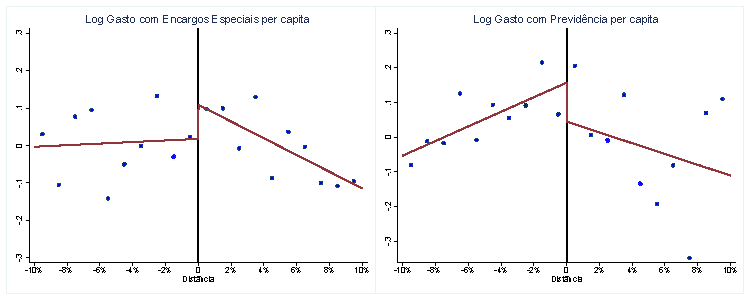
\includegraphics[width=15cm]{Graph5.pdf} %
    \begin{flushleft}
        \vspace{-0.4cm}
        \hspace{1.3cm}
    Fonte: Elaboração própria com base nos dados do IBGE e STN
    \end{flushleft}
    \label{funcao3}%
\end{figure}

Como outro experimento sobre as bases fiscais desses municípios, testou-se o impacto da descontinuidade em 2016, que foi o ano eleitoral dos municípios. Os resultados não mudam, pelo contrário, eles se tornam mais consistentes e os efeitos da descontinuidade aumenta. Ou seja, durante o ano eleitoral os gastos com a prefeitura municipal aumenta com o acrescimento de receita exógena.

\subsection{Índice Firjan de Gestão Fiscal}

Como já foi retratado anteriormente, além dos resultados gerais também foram adotadas medidas que buscam deixar os resultados principais mais robustos. O objetivo é analisar diversos tipos de situações e averiguar se o comportamento dos resultados mudam. % \citeonline{lee2010regression} afirmam que o uso de co-variadas podem reduzir a variância do estimador do efeito de tratamento; a possibilidade de correlação entre ser tratado e outras variáveis. Por outro lado, sob a hipótese de enquadramento imperfeito, torna útil o uso de co-variadas para mitigação de viés \cite{litschig2013impact}.

%correlação entre ser tratado?

% Ou seja, a inclusão das co-variadas gera problemas na estimação se tiverem significância com a política de transferência. Os resultados do apêndice mostram pelo teste das co-variadas que mesmo que algumas variáveis como emprego e empregados apresente significância numa banda de largura maior, seus resultados não são significantes para as bandas de larguras menores. Como os gastos com administrativo são significativos em todas as bandas e com e sem co variada, é possível afirmar que esse viés não está afetando os resultados de forma a que os mesmos se tornem inconclusivos.

% Também é importante incluir dentro das co-variadas a defasagem espacial. A inclusão desta variável nos permite detectar a existência de algum tipo de "efeito vizinhança", considerando que o município vizinho pode afetar o orçamento local. As demais variáveis incluídas foram selecionadas, tendo em vista fatores determinantes para a despesa pública em cada função. Nos resultados, é possível afirmar que o PIB afeta consideravelmente os municípios, bem como a distância do município em relação a capital, IFDM, variáveis políticas, empresas e empregabilidade.

Além das estimações realizadas, a análise foi complementada com as estimações das variáveis que determinam o Índice Firjan de Gestão Fiscal. O objetivo dessa seção é buscar mais consistência nos resultados obtidos.

Os resultados parecem indicar os mesmos efeitos já encontrados, mas pouco significantes, uma vez que o indicador de autonomia apresentou descontinuidade negativa. Pela criação do indicador, sabe-se que, o município só terá desempenho melhor se sua receita própria seja maior e possuam condições de arcar com administrativo e Legislativo. Contudo, os resultados anteriores indicaram que o acréscimo de receita exógena não gera nenhum tipo de incentivo na arrecadação própria e tem fortes indícios que a descontinuidade no administrativo é positivo e significativo. Assim, mesmo que esses resultados não sejam conclusivos, a significância estatística sob a descontinuidade negativa do indicador de autonomia pode ser explicada por essas vias.

\begin{figure}[H]%
    \centering
    \caption{Descontinuidade dos Indicadores de Gestão Fiscal}%
    \includegraphics[width=15cm]{Graph7.pdf} %
    \begin{flushleft}
        \vspace{-0.4cm}
        \hspace{1.3cm}
    Fonte: Elaboração própria com base nos dados do IBGE e STN
    \end{flushleft}
    \label{funcao}%
\end{figure}

\section{Considerações Finais}

Nos últimos anos, o Brasil e outros países optaram por adotar políticas de descentralização e seguir os pressupostos da Teoria Normativa, que afirma que países grandes devem ceder maiores responsabilidades a seus governos subnacionais por conta das suas devidas capacidades de atingir maior nível de eficiência.

Já que a capacidade de arrecadação tributária do município é pequena, o município é responsável pela provisão de segurança local, saúde básica, saneamento e educação (ensino infantil e anos iniciais do ensino fundamental). Por consequência, é de se esperar que os ganhos de transferências obtidos do governo central gerem incentivos benéficos e ampliem os gastos nas áreas básicas. A importância dos gastos nessas áreas se dá pela consolidação da literatura, que afirma que tanto a educação como também a saúde geram significativos ganhos de externalidade populacional e aumento de capital humano futuro.

Poderia uma arrecadação inesperada de recursos deteriorar a qualidade do gasto público? Essa questão é importante, uma vez que a forma como os municípios utilizam esses recursos podem gerar um impacto diferente de longo prazo. A expectativa é que as regiões mais atrasadas que receberam fundos adicionais compensem seu subdesenvolvimento no longo prazo.

Por isso, o objetivo com esta pesquisa é encontrar o comportamento dos municípios próximos à faixa do FPM com os seus gastos. As hipóteses são que os gastos na função educação e saúde positivamente associado com os ganhos de FPM nos indica gastos benéficos; gasto em Pessoal e em administrativo positivamente associado aos ganhos de FPM, nos indica resultados de desperdício de despesa, resultando em gastos maléficos. Em relação as receitas foi testado se as transferências podem gerar algum tipo de incentivo benéfico, uma vez que elas podem gerar algum tipo "preguiça fiscal" em relação às receitas próprias. É de se esperar que por seguir a Teoria Normativa, o Brasil adquira ganhos de eficiência com a política de transferência.

Ainda nesta pesquisa, também tentou-se evidenciar como a existência dos vizinhos podem impactar no comportamento do município. As estimações econométricas lineares utilizando a abordagem \textit{sharp} foram realizadas em várias situações possíveis: para três primeiros limiares juntos,  apenas os dois primeiros limiares e cada limiar individual. Os intervalos para cada estimação são de 2\%, 3\%, 4\% e 15\% das respectivas faixas populacionais. As especificações alternam a inclusão ou ausência de co-variadas.

Os resultados apresentados deste trabalho sugerem que as comunidades que receberam maior incentivo fiscal do governo central utilizaram grande parte desses recursos na função administrativa. Vale salientar que o aumento do gasto público teve como possível canal os gastos com pessoal, que pode nos indicar um possível resultado de incentivo perverso, uma vez que o município não utiliza seus ganhos adicionais de receitas em investimentos como saúde e educação.

Como em qualquer análise de descontinuidade de regressão, os impactos apresentados neste trabalho aplica-se apenas a municípios com níveis populacionais nos respectivos pontos de corte. No entanto, como os resultados são semelhantes entre os limiares, parece provável que os efeitos aqui apresentados generalizem para pelo menos o grupo de pequenos municípios (aqueles com população aproximada de 8.500 a 32.700), que representava cerca de 30\% dos municípios brasileiros em 2016.

% O uso de estimadores envolvendo repasses e o orçamento municipal, sem controles adicionais, podem trazer algum tipo de viés. Torna-se, então, necessário encontrar uma variável exógena que não varie estritamente em face da demanda por parte dos beneficiários, mas oferte recursos com algum grau de aleatoriedade. Por hipótese, assume-se que os municípios próximos às faixas de coeficientes do FPM são homogêneos entre os grupos de controle (municípios abaixo do limite) e tratamento (municípios acima do limite). Portanto, eventuais diferenças entre eles podem ser atribuídas às transferências federais.

Muitos trabalhos anteriores buscam analisar o impacto desses recursos adicionais nas condições sociais e econômicas do município, mas, assim como foi proposto, este trabalho também vê como importante buscar evidências de qual incentivo estes recursos geram no orçamento destes municípios. Em princípio, existem outros mecanismos que podem interagir com nossos resultados e contribuir para explicar o impacto de transferências maiores, como a análise do crescimento econômico e desigualdade social. Os resultados obtidos indicam os seguintes fatores:

\begin{itemize}
    \item Acréscimos de receita exógeno geram aumentos de gastos com pessoal. Este resultado torna significativo apenas com a inclusão das co-variadas.
    \item Forte significância estatística dos gastos com administrativo. Os aumentos dos gastos com pessoal situam como os gastos com administrativo estão sendo realizados.
    \item Por outro lado, os demais gastos, como despesa com educação, saúde, segurança pública e transporte não apresentaram sofrer nenhum impacto das transferências adicionais do FPM. 
    \item O gasto defasado espacialmente mostra-se relevante para o impacto do gasto local.
    \item Em 2016 (ano eleitoral) os resultados se repetem e apresentam coeficientes mais intensos quando são comparados com os resultados do painel (gestão completa).
    \item Apesar de não ser muito significativo, a descontinuidade do indicador de Autonomia do Índice Firjan de Gestão Fiscal da indícios da perda de eficiência da descontinuidade positiva dos gastos na administração pública da prefeitura na autonomia municipal.
\end{itemize}

Estes resultados servem para contribuir na literatura recente que analisa o impacto das transferências constitucionais do FPM no desenvolvimento municipal. Outras análises poderiam ser aplicadas a esta pesquisa, como inclusão de outras variáveis de controle como climáticas, controle do gasto defasado espacial para municípios pequenos ou grandes (vizinhos) e explorar seria as estimações dos resultados pelo \textit{fuzzy} RDD.

O fato desta análise se limitar a um período específico e apenas para pequenos municípios fazem com que esta pesquisa perca um pouco sua validade externa. Isto é, este experimento se torna conclusivo apenas para este período de tempo para estes municípios em questão. A expectativa é que para pesquisas futuras sejam exploradas esses efeitos para um período maior. Estes resultados servem para que os gestores e a população local reflitam sobre como as políticas públicas estão sendo aplicadas e quais as implicações da mesma a curto e longo prazo.

\newpage

\bibliography{referencias.bib}

\newpage

\begin{appendices}

\chapter{Resultados econométricos}
\label{appendix:graph}
\vspace{-1.6cm}

\begin{figure}[H]
    \centering
    \caption{Distribuição dos municípios pequenos por nível de receita do FPM per Capita}
    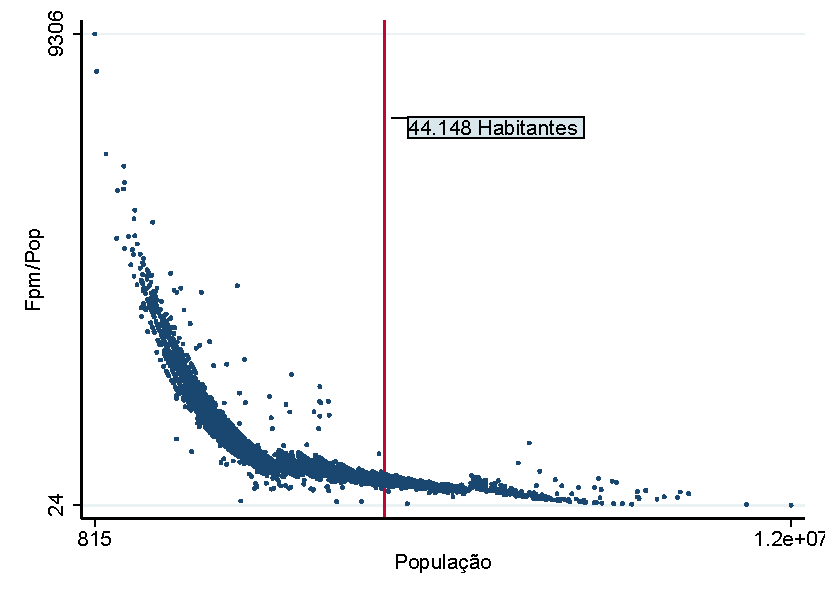
\includegraphics{Fpmpop.pdf}
        \begin{flushleft}
        \vspace{-0.4cm}
        \hspace{1.3cm}
    Fonte: Elaboração própria com base nos dados do IBGE
    \end{flushleft}
    \label{mun_per_capita}%
    \label{fig:my_label}
\end{figure}

\begin{figure}[H]%
    \centering
    \caption{Teste de manipulação populacional - 1º Janela}%
    \includegraphics[width=15cm]{graph_teste1.pdf} %
        \begin{flushleft}
        \vspace{-0.4cm}
        \hspace{0.4cm}
    Fonte: Elaboração própria com base nos dados do IBGE
    \end{flushleft}
    \label{mccrary1}%
\end{figure}

\begin{figure}[H]%
    \centering
    \caption{Teste de manipulação populacional - 2º Janela}%
    \includegraphics[width=15cm]{graph_teste2.pdf} %
        \begin{flushleft}
        \vspace{-0.4cm}
        \hspace{0.4cm}
    Fonte: Elaboração própria com base nos dados do IBGE
    \end{flushleft}
    \label{mccrary2}%
\end{figure}

\begin{figure}[H]%
    \centering
    \caption{Teste de manipulação populacional - 3º Janela}%
    \includegraphics[width=15cm]{graph_teste3.pdf} %
        \begin{flushleft}
        \vspace{-0.4cm}
        \hspace{0.4cm}
    Fonte: Elaboração própria com base nos dados do IBGE
    \end{flushleft}
    \label{mccrary3}%
\end{figure}

\begin{figure}[H]%
    \centering
    \caption{Teste de Placebo para população na faixa de 5000 e 20000 habitantes}%
    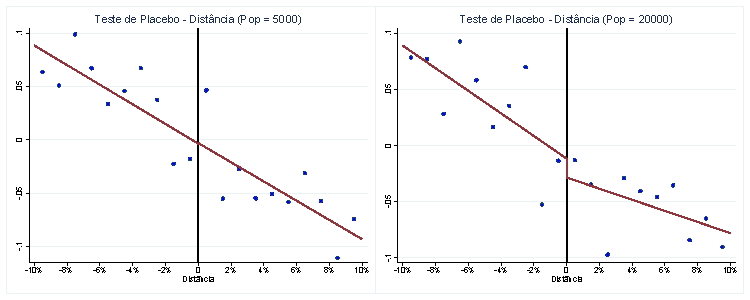
\includegraphics[width=15cm]{Teste_Placebo.pdf} %
        \begin{flushleft}
        \vspace{-0.4cm}
        \hspace{0.4cm}
    Fonte: Elaboração própria com base nos dados do IBGE
    \end{flushleft}
    \label{placebo}%
\end{figure}

\begin{table}[H] 
  \hspace{-1.5cm}
  \centering
  \caption{Teste de descontinuidade para as covariadas}
  \begin{tabular}{l*{4}{c}}
  \hline
  \textit{Bandwidth} &\multicolumn{1}{c}{4\%}&\multicolumn{1}{c}{5\%}&\multicolumn{1}{c}{10\%}&\multicolumn{1}{c}{15\%}\\
  \hline
  \multicolumn{4}{l}{\textbf{Distância}}\\
   & -29.017 & -30.150 & -18.666 & -7.257 \\
 & (21.408) & (18.877) & (13.132) & (11.453) \\
Observations & 1,687 & 2,117 & 4,478 & 6,130 \\
  \hline
    \multicolumn{4}{l}{\textbf{Empresas}}\\
   & -25.364 & -15.826 & -32.598* & -31.914** \\
 & (28.409) & (25.586) & (17.884) & (15.994) \\
Observations & 1,687 & 2,117 & 4,478 & 6,130 \\
  \hline
    \multicolumn{4}{l}{\textbf{Empregados}}\\
   & -251.141 & -111.690 & -182.863* & -177.522** \\
 & (160.400) & (140.284) & (97.228) & (83.912) \\
Observations & 1,687 & 2,117 & 4,478 & 6,130 \\
  \hline
  \multicolumn{4}{l}{\textbf{PIB}}\\
   & -324.616 & -222.925 & -85.410 & -161.430 \\
 & (354.297) & (313.694) & (271.761) & (267.278) \\
Observations & 1,687 & 2,117 & 4,478 & 6,130 \\
  \hline
  \multicolumn{4}{l}{\textbf{Possibilidade de Reeleição}}\\
   & 0.043 & 0.056 & 0.062* & 0.017 \\
 & (0.057) & (0.051) & (0.036) & (0.032) \\
Observations & 1,687 & 2,117 & 4,478 & 6,130 \\
  \hline
  \multicolumn{5}{l}{\footnotesize \sym{*} 10\% de significância estatística} \\
  \multicolumn{5}{l}{\footnotesize \sym{**} 5\% de significância estatística} \\
  \multicolumn{5}{l}{\footnotesize \sym{***} 1\% de significância estatística}
\end{tabular}
\end{table}

\begin{table}[H] \footnotesize 
  \hspace{-1.5cm}
  \centering
  \caption{RD para Receita total per capita}
  \begin{tabular}{l*{8}{c}} 
  \hline
  \multicolumn{8}{l}{\textbf{Variável Dependente: Log Receita per capita}}\\
  \hline
  Equação &\multicolumn{1}{c}{(1)}&\multicolumn{1}{c}{(2)}&\multicolumn{1}{c}{(3)}&\multicolumn{1}{c}{(4)}&\multicolumn{1}{c}{(5)}&\multicolumn{1}{c}{(6)}&\multicolumn{1}{c}{(7)}&\multicolumn{1}{c}{(8)}\\
  \textit{Bandwidth} &\multicolumn{1}{c}{4\%}&\multicolumn{1}{c}{4\%}&\multicolumn{1}{c}{5\%}&\multicolumn{1}{c}{5\%}&\multicolumn{1}{c}{10\%}&\multicolumn{1}{c}{10\%}&\multicolumn{1}{c}{15\%}&\multicolumn{1}{c}{15\%}\\
  \hline
\textit{Painel: 1-3 Janelas}   &  &  &  &  &  &  &  &  \\
$[X > 0]$ & 0.094** & 0.107*** & 0.079** & 0.072*** & 0.062*** & 0.042** & 0.058*** & 0.048*** \\
 & (0.037) & (0.035) & (0.031) & (0.020) & (0.023) & (0.018) & (0.020) & (0.017) \\
Observations & 1,622 & 1,622 & 1,373 & 2,032 & 2,909 & 4,303 & 4,051 & 5,883 \\
 R-squared & 0.224 & 0.294 & 0.348 & 0.312 & 0.379 & 0.375 & 0.409 & 0.343 \\ \hline
\textit{Painel: 1-2 Janelas} &  &  &  &  &  &  &  &  \\
$[X > 0]$ & 0.110*** & 0.126*** & 0.079** & 0.105*** & 0.062*** & 0.076*** & 0.058*** & 0.064*** \\
 & (0.039) & (0.034) & (0.031) & (0.025) & (0.023) & (0.019) & (0.020) & (0.017) \\
Observations & 1,112 & 1,112 & 1,373 & 1,373 & 2,909 & 2,908 & 4,051 & 4,050 \\
 R-squared & 0.338 & 0.488 & 0.348 & 0.502 & 0.379 & 0.527 & 0.409 & 0.556 \\ \hline
\textit{Painel: 1º Janela}  &  &  &  &  &  &  &  &  \\
I[Pop > 10,188] & 0.066 & 0.067* & 0.057 & 0.069** & 0.044 & 0.059** & 0.039 & 0.045** \\
 & (0.056) & (0.039) & (0.051) & (0.033) & (0.036) & (0.024) & (0.029) & (0.021) \\
Observations & 554 & 554 & 687 & 687 & 1,482 & 1,482 & 2,239 & 2,239 \\
 R-squared & 0.463 & 0.736 & 0.462 & 0.718 & 0.426 & 0.618 & 0.441 & 0.619 \\ \hline
\textit{Painel: 2º Janela}  &  &  &  &  &  &  &  &  \\
I[Pop > 13,584] & 0.086* & 0.113** & 0.064 & 0.100*** & 0.074** & 0.079*** & 0.077*** & 0.073*** \\
 & (0.048) & (0.047) & (0.041) & (0.038) & (0.031) & (0.028) & (0.029) & (0.026) \\
Observations & 558 & 558 & 686 & 686 & 1,427 & 1,426 & 1,812 & 1,811 \\
 R-squared & 0.321 & 0.378 & 0.325 & 0.404 & 0.362 & 0.489 & 0.397 & 0.522 \\ \hline
\textit{Painel: 3º Janela}  &  &  &  &  &  &  &  &  \\
I[Pop > 16,980] & 0.088 & 0.091 & 0.032 & 0.021 & -0.027 & -0.025 & 0.015 & 0.015 \\
 & (0.108) & (0.108) & (0.043) & (0.038) & (0.043) & (0.043) & (0.043) & (0.043) \\
Observations & 510 & 510 & 659 & 659 & 1,396 & 1,395 & 1,834 & 1,833 \\
 R-squared & 0.189 & 0.211 & 0.186 & 0.214 & 0.205 & 0.248 & 0.173 & 0.208 \\ \hline
  Controle       &         Não         &         Sim         &         Não         &         Sim         &         Não         &         Sim         &        Não         &        Sim         \\
  \hline
  \multicolumn{9}{p{42.5em}}{\footnotesize Estatística MQO: Erros padrão robustos de heterocedasticidade entre parênteses. O \textit{bandwidth} (\%) é a distância percentual do respectivo ponto de corte. Todas as especificações incluem efeitos fixos do estado. As especificações agrupadas incluem manequins de segmento. As covariáveis de pré-tratamento incluem o PIB Per Capita do Município per capita, dummy de reeleição, Índice Firjan de Desenvolvimento Municipal, número de industrias, número de empresas e a defasagem espacial.}\\
  \multicolumn{9}{l}{\footnotesize \sym{*} 10\% de significância estatística} \\
  \multicolumn{9}{l}{\footnotesize \sym{**} 5\% de significância estatística} \\
  \multicolumn{9}{l}{\footnotesize \sym{***} 1\% de significância estatística}
\end{tabular} \label{gasto_table}
\end{table}

\begin{table}[H] \footnotesize 
  \hspace{-1.5cm}
  \centering
  \caption{RD para gastos municipais per capita}
  \begin{tabular}{l*{8}{c}} 
  \hline
  \multicolumn{8}{l}{\textbf{Variável Dependente: Log Despesa per capita}}\\
  \hline
  Equação &\multicolumn{1}{c}{(1)}&\multicolumn{1}{c}{(2)}&\multicolumn{1}{c}{(3)}&\multicolumn{1}{c}{(4)}&\multicolumn{1}{c}{(5)}&\multicolumn{1}{c}{(6)}&\multicolumn{1}{c}{(7)}&\multicolumn{1}{c}{(8)}\\
  \textit{Bandwidth} &\multicolumn{1}{c}{4\%}&\multicolumn{1}{c}{4\%}&\multicolumn{1}{c}{5\%}&\multicolumn{1}{c}{5\%}&\multicolumn{1}{c}{10\%}&\multicolumn{1}{c}{10\%}&\multicolumn{1}{c}{15\%}&\multicolumn{1}{c}{15\%}\\
  \hline
\textit{Painel: 1-3 Janelas}  &  &  &  &  &  &  &  &  \\
$[X > 0]$ & 0.069** & 0.081** & 0.053* & 0.052*** & 0.068*** & 0.047*** & 0.056*** & 0.046*** \\
 & (0.034) & (0.031) & (0.028) & (0.019) & (0.021) & (0.017) & (0.018) & (0.016) \\
Observations & 1,624 & 1,624 & 1,374 & 2,032 & 2,910 & 4,305 & 4,052 & 5,890 \\
R-squared & 0.227 & 0.296 & 0.445 & 0.317 & 0.453 & 0.391 & 0.475 & 0.343 \\ \hline
\textit{Painel: 1-2 Janelas} &  &  &  &  &  &  &  &  \\
$[X > 0]$ & 0.081** & 0.094*** & 0.053* & 0.076*** & 0.068*** & 0.080*** & 0.056*** & 0.061*** \\
 & (0.032) & (0.026) & (0.028) & (0.023) & (0.021) & (0.017) & (0.018) & (0.014) \\
Observations & 1,114 & 1,114 & 1,374 & 1,374 & 2,910 & 2,909 & 4,052 & 4,051 \\
 R-squared & 0.449 & 0.643 & 0.445 & 0.640 & 0.453 & 0.623 & 0.475 & 0.639 \\ \hline
\textit{Painel: 1º Janela} &  &  &  &  &  &  &  &  \\
I[Pop > 10,188] & 0.060 & 0.059 & 0.046 & 0.056 & 0.050 & 0.063** & 0.030 & 0.037* \\
 & (0.057) & (0.045) & (0.051) & (0.039) & (0.035) & (0.027) & (0.028) & (0.021) \\
Observations & 555 & 555 & 687 & 687 & 1,483 & 1,483 & 2,241 & 2,241 \\ \hline
\textit{Painel: 2º Janela} &  &  &  &  &  &  &  &  \\
I[Pop > 13,584] & 0.055* & 0.082*** & 0.034 & 0.061** & 0.079*** & 0.084*** & 0.082*** & 0.077*** \\
 & (0.034) & (0.030) & (0.031) & (0.027) & (0.023) & (0.020) & (0.021) & (0.018) \\
Observations & 559 & 559 & 687 & 687 & 1,427 & 1,426 & 1,811 & 1,810 \\
 R-squared & 0.565 & 0.673 & 0.550 & 0.689 & 0.496 & 0.690 & 0.517 & 0.695 \\ \hline
\textit{Painel: 3º Janela} &  &  &  &  &  &  &  &  \\
I[Pop > 16,980] & 0.074 & 0.078 & 0.026 & 0.013 & -0.030 & -0.028 & 0.008 & 0.009 \\
 & (0.108) & (0.108) & (0.042) & (0.038) & (0.043) & (0.042) & (0.042) & (0.042) \\
Observations & 510 & 510 & 658 & 658 & 1,397 & 1,396 & 1,840 & 1,839 \\
 R-squared & 0.172 & 0.193 & 0.169 & 0.196 & 0.189 & 0.234 & 0.157 & 0.191 \\ \hline
  Controle       &         Não         &         Sim         &         Não         &         Sim         &         Não         &         Sim         &        Não         &        Sim         \\
  \hline
  \multicolumn{9}{p{42.5em}}{\footnotesize Estatística MQO: Erros padrão robustos de heterocedasticidade entre parênteses. O \textit{bandwidth} (\%) é a distância percentual do respectivo ponto de corte. Todas as especificações incluem efeitos fixos do estado. As especificações agrupadas incluem manequins de segmento. As covariáveis de pré-tratamento incluem o PIB Per Capita do Município per capita, dummy de reeleição, Índice Firjan de Desenvolvimento Municipal, número de industrias, número de empresas e a defasagem espacial.}\\
  \multicolumn{9}{l}{\footnotesize \sym{*} 10\% de significância estatística} \\
  \multicolumn{9}{l}{\footnotesize \sym{**} 5\% de significância estatística} \\
  \multicolumn{9}{l}{\footnotesize \sym{***} 1\% de significância estatística}
\end{tabular} \label{gasto_table}
\end{table}

\begin{table}[H] \small 
  \hspace{-1.5cm}
  \centering
  \caption{RD para gastos municipais com Pessoal per capita}
  \begin{tabular}{l*{8}{c}}
  \hline
  \multicolumn{8}{l}{\textbf{Variável Dependente: Log Gasto com Pessoal per capita}}\\
  \hline
  Equação &\multicolumn{1}{c}{(1)}&\multicolumn{1}{c}{(2)}&\multicolumn{1}{c}{(3)}&\multicolumn{1}{c}{(4)}&\multicolumn{1}{c}{(5)}&\multicolumn{1}{c}{(6)}&\multicolumn{1}{c}{(7)}&\multicolumn{1}{c}{(8)}\\
  \textit{Bandwidth} &\multicolumn{1}{c}{4\%}&\multicolumn{1}{c}{4\%}&\multicolumn{1}{c}{5\%}&\multicolumn{1}{c}{5\%}&\multicolumn{1}{c}{10\%}&\multicolumn{1}{c}{10\%}&\multicolumn{1}{c}{15\%}&\multicolumn{1}{c}{15\%}\\
  \hline
\textit{Painel: 1-3 Janelas}  &  &  &  &  &  &  &  &  \\
$[X > 0]$ & 0.061* & 0.071** & 0.043* & 0.045** & 0.038** & 0.029* & 0.031* & 0.028* \\
 & (0.032) & (0.030) & (0.025) & (0.018) & (0.019) & (0.017) & (0.017) & (0.016) \\
Observations & 1,622 & 1,622 & 1,373 & 2,030 & 2,907 & 4,301 & 4,049 & 5,886 \\
 R-squared & 0.252 & 0.306 & 0.498 & 0.324 & 0.484 & 0.398 & 0.499 & 0.347 \\ \hline
\textit{Painel: 1-2 Janelas} &  &  &  &  &  &  &  &  \\
$[X > 0]$ & 0.059** & 0.068*** & 0.043* & 0.062*** & 0.038** & 0.051*** & 0.031* & 0.037*** \\
 & (0.028) & (0.025) & (0.025) & (0.022) & (0.019) & (0.016) & (0.017) & (0.014) \\
Observations & 1,113 & 1,113 & 1,373 & 1,373 & 2,907 & 2,906 & 4,049 & 4,048 \\
 R-squared & 0.516 & 0.660 & 0.498 & 0.643 & 0.484 & 0.607 & 0.499 & 0.616 \\ \hline
 \textit{Painel: 1º Janela} &  &  &  &  &  &  &  &  \\
I[Pop > 10,188] & 0.035 & 0.033 & 0.034 & 0.044 & 0.014 & 0.023 & 0.001 & 0.006 \\
 & (0.045) & (0.037) & (0.041) & (0.034) & (0.030) & (0.024) & (0.024) & (0.020) \\
Observations & 554 & 554 & 686 & 686 & 1,481 & 1,481 & 2,238 & 2,238 \\
 R-squared & 0.534 & 0.703 & 0.505 & 0.664 & 0.493 & 0.616 & 0.507 & 0.627 \\ \hline
 \textit{Painel: 2º Janela} &  &  &  &  &  &  &  &  \\
I[Pop > 13,584] & 0.023 & 0.053* & 0.016 & 0.050* & 0.059** & 0.070*** & 0.060*** & 0.061*** \\
 & (0.035) & (0.032) & (0.032) & (0.028) & (0.024) & (0.021) & (0.022) & (0.019) \\
Observations & 559 & 559 & 687 & 687 & 1,426 & 1,425 & 1,811 & 1,810 \\
 R-squared & 0.576 & 0.676 & 0.561 & 0.681 & 0.518 & 0.677 & 0.523 & 0.669 \\ \hline
  \textit{Painel: 3º Janela} &  &  &  &  &  &  &  &  \\
I[Pop > 16,980] & 0.090 & 0.094 & 0.024 & 0.015 & -0.022 & -0.016 & 0.005 & 0.011 \\
 & (0.104) & (0.105) & (0.043) & (0.040) & (0.042) & (0.042) & (0.041) & (0.042) \\
Observations & 509 & 509 & 657 & 657 & 1,396 & 1,395 & 1,839 & 1,838 \\
 R-squared & 0.175 & 0.191 & 0.177 & 0.196 & 0.214 & 0.247 & 0.174 & 0.200 \\ \hline
  Controle       &         Não         &         Sim         &         Não         &         Sim         &         Não         &         Sim         &        Não         &        Sim         \\
  \hline
  \multicolumn{9}{p{42.5em}}{\footnotesize Estatística MQO: Erros padrão robustos de heterocedasticidade entre parênteses. O \textit{bandwidth} (\%) é a distância percentual do respectivo ponto de corte. Todas as especificações incluem efeitos fixos do estado. As especificações agrupadas incluem manequins de segmento. As covariáveis de pré-tratamento incluem o PIB Per Capita do Município per capita, dummy de reeleição, Índice Firjan de Desenvolvimento Municipal, número de industrias, número de empresas e a defasagem espacial.}\\
  \multicolumn{9}{l}{\footnotesize \sym{*} 10\% de significância estatística} \\
  \multicolumn{9}{l}{\footnotesize \sym{**} 5\% de significância estatística} \\
  \multicolumn{9}{l}{\footnotesize \sym{***} 1\% de significância estatística}
\end{tabular} \label{tabela_pessoal}
\end{table}

\begin{table}[H] \small
  \centering
  \caption{RD para gastos municipais com Capital per capital}
\begin{tabular}{l*{8}{c}}
\hline
\multicolumn{8}{l}{\textbf{Variável Dependente: Log Gasto com Capital per capita}}\\
\hline
Equação &\multicolumn{1}{c}{(1)}&\multicolumn{1}{c}{(2)}&\multicolumn{1}{c}{(3)}&\multicolumn{1}{c}{(4)}&\multicolumn{1}{c}{(5)}&\multicolumn{1}{c}{(6)}&\multicolumn{1}{c}{(7)}&\multicolumn{1}{c}{(8)}\\
  \textit{Bandwidth} &\multicolumn{1}{c}{4\%}&\multicolumn{1}{c}{4\%}&\multicolumn{1}{c}{5\%}&\multicolumn{1}{c}{5\%}&\multicolumn{1}{c}{10\%}&\multicolumn{1}{c}{10\%}&\multicolumn{1}{c}{15\%}&\multicolumn{1}{c}{15\%}\\
\hline
\textit{Painel: 1-3 Janelas}  &  &  &  &  &  &  &  &  \\
$[X > 0]$ & -0.020 & 0.001 & 0.007 & -0.014 & 0.112** & 0.078* & 0.064 & 0.061* \\
 & (0.069) & (0.067) & (0.076) & (0.059) & (0.053) & (0.041) & (0.045) & (0.035) \\
Observations & 1,620 & 1,620 & 1,370 & 2,026 & 2,905 & 4,294 & 4,047 & 5,878 \\
 R-squared & 0.214 & 0.264 & 0.194 & 0.256 & 0.172 & 0.229 & 0.187 & 0.238 \\ \hline
\textit{Painel: 1-2 Janelas} &  &  &  &  &  &  &  &  \\
$[X > 0]$ & 0.060 & 0.085 & 0.007 & 0.034 & 0.112** & 0.121** & 0.064 & 0.069 \\
 & (0.087) & (0.084) & (0.076) & (0.073) & (0.053) & (0.051) & (0.045) & (0.044) \\
Observations & 1,111 & 1,111 & 1,370 & 1,370 & 2,905 & 2,904 & 4,047 & 4,046 \\
 R-squared & 0.207 & 0.261 & 0.194 & 0.250 & 0.172 & 0.212 & 0.187 & 0.230 \\ \hline
\textit{Painel: 1º Janela} &  &  &  &  &  &  &  &  \\
I[Pop > 10,188] & -0.002 & 0.032 & -0.019 & -0.001 & 0.135 & 0.151* & 0.055 & 0.063 \\
 & (0.144) & (0.137) & (0.123) & (0.116) & (0.084) & (0.079) & (0.066) & (0.063) \\
Observations & 553 & 553 & 685 & 685 & 1,481 & 1,481 & 2,238 & 2,238 \\
 R-squared & 0.234 & 0.317 & 0.218 & 0.300 & 0.185 & 0.237 & 0.189 & 0.241 \\ \hline
\textit{Painel: 2º Janela} &  &  &  &  &  &  &  &  \\
I[Pop > 13,584] & 0.083 & 0.106 & 0.003 & 0.030 & 0.065 & 0.063 & 0.055 & 0.045 \\
 & (0.109) & (0.109) & (0.098) & (0.097) & (0.068) & (0.067) & (0.061) & (0.061) \\
Observations & 558 & 558 & 685 & 685 & 1,424 & 1,423 & 1,809 & 1,808 \\
 R-squared & 0.233 & 0.256 & 0.211 & 0.243 & 0.179 & 0.228 & 0.197 & 0.246 \\ \hline
\textit{Painel: 3º Janela} &  &  &  &  &  &  &  &  \\
I[Pop > 16,980] & -0.169 & -0.150 & -0.082 & -0.087 & -0.007 & 0.001 & 0.032 & 0.038 \\
 & (0.108) & (0.104) & (0.100) & (0.096) & (0.071) & (0.069) & (0.061) & (0.059) \\
Observations & 509 & 509 & 656 & 656 & 1,391 & 1,390 & 1,833 & 1,832 \\
 R-squared & 0.303 & 0.362 & 0.283 & 0.343 & 0.234 & 0.296 & 0.229 & 0.288 \\ \hline
\hline
Controle       &         Não         &         Sim         &         Não         &         Sim         &         Não         &         Sim         &        Não         &        Sim         \\
\hline
  \multicolumn{9}{p{42.5em}}{\footnotesize Estatística MQO: Erros padrão robustos de heterocedasticidade entre parênteses. O \textit{bandwidth} (\%) é a distância percentual do respectivo ponto de corte. Todas as especificações incluem efeitos fixos do estado. As especificações agrupadas incluem manequins de segmento. As covariáveis de pré-tratamento incluem o PIB Per Capita do Município per capita, dummy de reeleição, Índice Firjan de Desenvolvimento Municipal, número de industrias, número de empresas e a defasagem espacial.}\\
  \multicolumn{9}{l}{\footnotesize \sym{*} 10\% de significância estatística} \\
  \multicolumn{9}{l}{\footnotesize \sym{**} 5\% de significância estatística} \\
  \multicolumn{9}{l}{\footnotesize \sym{***} 1\% de significância estatística}
  \end{tabular}
\end{table}

\begin{table}[H] \small
  \centering
  \caption{RD para gastos municipais com Educação per capita}
\begin{tabular}{l*{8}{c}}
\hline
\multicolumn{8}{l}{\textbf{Variável Dependente: Log Gasto em Educação per capita}}\\
\hline
Equação &\multicolumn{1}{c}{(1)}&\multicolumn{1}{c}{(2)}&\multicolumn{1}{c}{(3)}&\multicolumn{1}{c}{(4)}&\multicolumn{1}{c}{(5)}&\multicolumn{1}{c}{(6)}&\multicolumn{1}{c}{(7)}&\multicolumn{1}{c}{(8)}\\
  \textit{Bandwidth} &\multicolumn{1}{c}{4\%}&\multicolumn{1}{c}{4\%}&\multicolumn{1}{c}{5\%}&\multicolumn{1}{c}{5\%}&\multicolumn{1}{c}{10\%}&\multicolumn{1}{c}{10\%}&\multicolumn{1}{c}{15\%}&\multicolumn{1}{c}{15\%}\\
\hline
\textit{Painel: 1-3 Janelas}  &  &  &  &  &  &  &  &  \\
$[X > 0]$ & 0.010 & 0.025 & -0.009 & 0.006 & 0.015 & 0.025 & 0.014 & 0.023 \\
 & (0.029) & (0.026) & (0.035) & (0.024) & (0.025) & (0.018) & (0.022) & (0.015) \\
Observations & 1,607 & 1,607 & 1,366 & 2,013 & 2,887 & 4,264 & 4,022 & 5,836 \\
 R-squared & 0.446 & 0.541 & 0.398 & 0.513 & 0.421 & 0.527 & 0.436 & 0.536 \\ \hline
\textit{Painel: 1-2 Janelas} &  &  &  &  &  &  &  &  \\
$[X > 0]$ & 0.031 & 0.056* & -0.009 & 0.022 & 0.015 & 0.030 & 0.014 & 0.021 \\
 & (0.038) & (0.034) & (0.035) & (0.032) & (0.025) & (0.023) & (0.022) & (0.020) \\
Observations & 1,107 & 1,107 & 1,366 & 1,366 & 2,887 & 2,886 & 4,022 & 4,021 \\
 R-squared & 0.421 & 0.548 & 0.398 & 0.503 & 0.421 & 0.508 & 0.436 & 0.525 \\ \hline
\textit{Painel: 1º Janela} &  &  &  &  &  &  &  &  \\
I[Pop > 10,188] & 0.033 & 0.061 & 0.022 & 0.048 & -0.003 & 0.001 & -0.021 & -0.020 \\
 & (0.063) & (0.049) & (0.056) & (0.044) & (0.040) & (0.034) & (0.031) & (0.026) \\
Observations & 551 & 551 & 683 & 683 & 1,468 & 1,468 & 2,221 & 2,221 \\
 R-squared & 0.389 & 0.590 & 0.392 & 0.577 & 0.421 & 0.538 & 0.450 & 0.563 \\ \hline
\textit{Painel: 2º Janela} &  &  &  &  &  &  &  &  \\
I[Pop > 13,584] & -0.014 & 0.012 & -0.068 & -0.036 & 0.021 & 0.037 & 0.049 & 0.057* \\
 & (0.045) & (0.045) & (0.046) & (0.047) & (0.032) & (0.031) & (0.030) & (0.029) \\
Observations & 556 & 556 & 683 & 683 & 1,419 & 1,418 & 1,801 & 1,800 \\
 R-squared & 0.528 & 0.577 & 0.448 & 0.493 & 0.446 & 0.519 & 0.443 & 0.514 \\ \hline
\textit{Painel: 3º Janela} &  &  &  &  &  &  &  &  \\
I[Pop > 16,980] & -0.026 & -0.029 & -0.012 & -0.023 & 0.011 & 0.013 & 0.027 & 0.031 \\
 & (0.042) & (0.040) & (0.038) & (0.036) & (0.027) & (0.026) & (0.024) & (0.023) \\
Observations & 500 & 500 & 647 & 647 & 1,379 & 1,378 & 1,816 & 1,815 \\
 R-squared & 0.584 & 0.634 & 0.588 & 0.640 & 0.544 & 0.600 & 0.540 & 0.594 \\ \hline
Controle       &         Não         &         Sim         &         Não         &         Sim         &         Não         &         Sim         &        Não         &        Sim         \\
\hline
  \multicolumn{9}{p{42.5em}}{\footnotesize Estatística MQO: Erros padrão robustos de heterocedasticidade entre parênteses. O \textit{bandwidth} (\%) é a distância percentual do respectivo ponto de corte. Todas as especificações incluem efeitos fixos do estado. As especificações agrupadas incluem manequins de segmento. As covariáveis de pré-tratamento incluem o PIB Per Capita do Município per capita, dummy de reeleição, Índice Firjan de Desenvolvimento Municipal, número de industrias, número de empresas e a defasagem espacial.}\\
  \multicolumn{9}{l}{\footnotesize \sym{*} 10\% de significância estatística} \\
  \multicolumn{9}{l}{\footnotesize \sym{**} 5\% de significância estatística} \\
  \multicolumn{9}{l}{\footnotesize \sym{***} 1\% de significância estatística}
\end{tabular}
\end{table}

\begin{table}[H] \small
  \centering
  \caption{RD para gastos municipais com Saúde per capita}
\begin{tabular}{l*{8}{c}}
\hline
\multicolumn{8}{l}{\textbf{Variável Dependente: Log Gasto em Saúde per capita}}\\
\hline
Equação &\multicolumn{1}{c}{(1)}&\multicolumn{1}{c}{(2)}&\multicolumn{1}{c}{(3)}&\multicolumn{1}{c}{(4)}&\multicolumn{1}{c}{(5)}&\multicolumn{1}{c}{(6)}&\multicolumn{1}{c}{(7)}&\multicolumn{1}{c}{(8)}\\
  \textit{Bandwidth} &\multicolumn{1}{c}{4\%}&\multicolumn{1}{c}{4\%}&\multicolumn{1}{c}{5\%}&\multicolumn{1}{c}{5\%}&\multicolumn{1}{c}{10\%}&\multicolumn{1}{c}{10\%}&\multicolumn{1}{c}{15\%}&\multicolumn{1}{c}{15\%}\\
\hline
\textit{Painel: 1-3 Janelas}  &  &  &  &  &  &  &  &  \\
$[X > 0]$ & 0.021 & 0.039 & 0.055 & 0.039 & 0.065** & 0.048** & 0.039 & 0.026 \\
 & (0.036) & (0.035) & (0.047) & (0.032) & (0.032) & (0.023) & (0.027) & (0.020) \\
Observations & 1,607 & 1,607 & 1,366 & 2,013 & 2,884 & 4,262 & 4,020 & 5,834 \\
 R-squared & 0.371 & 0.448 & 0.333 & 0.441 & 0.356 & 0.473 & 0.353 & 0.469 \\ \hline
\textit{Painel: 1-2 Janelas} &  &  &  &  &  &  &  &  \\
$[X > 0]$ & 0.061 & 0.088* & 0.055 & 0.091** & 0.065** & 0.084*** & 0.039 & 0.049* \\
 & (0.051) & (0.048) & (0.047) & (0.045) & (0.032) & (0.030) & (0.027) & (0.026) \\
Observations & 1,107 & 1,107 & 1,366 & 1,366 & 2,884 & 2,883 & 4,020 & 4,019 \\
 R-squared & 0.354 & 0.437 & 0.333 & 0.422 & 0.356 & 0.442 & 0.353 & 0.435 \\ \hline
\textit{Painel: 1º Janela} &  &  &  &  &  &  &  &  \\
I[Pop > 10,188] & -0.019 & 0.036 & -0.011 & 0.068 & -0.015 & 0.020 & -0.030 & -0.009   \\
 & (0.070) & (0.059) & (0.069) & (0.060) & (0.050) & (0.043) & (0.040) & (0.036)  \\
Observations & 552 & 552 & 684 & 684 & 1,468 & 1,468 & 2,222 & 2,222   \\
 R-squared & 0.3712 & 0.490 & 0.329 & 0.445 & 0.352 & 0.444 & 0.346 & 0.437 \\ \hline
\textit{Painel: 2º Janela} &  &  &  &  &  &  &  &  \\
I[Pop > 13,584] & 0.104 & 0.129* & 0.105 & 0.126* & 0.139*** & 0.138*** & 0.118*** & 0.110*** \\
 & (0.074) & (0.077) & (0.069) & (0.072) & (0.046) & (0.045) & (0.041) & (0.041) \\
Observations & 555 & 555 & 682 & 682 & 1,416 & 1,415 & 1,798 & 1,797 \\
 R-squared & 0.375 & 0.411 & 0.372 & 0.426 & 0.385 & 0.488 & 0.388 & 0.478 \\ \hline
 \textit{Painel: 3º Janela} &  &  &  &  &  &  &  &  \\
I[Pop > 16,980] & -0.094** & -0.089** & -0.067 & -0.079** & -0.037 & -0.036 & -0.040 & -0.041* \\
 & (0.046) & (0.042) & (0.041) & (0.039) & (0.029) & (0.027) & (0.025) & (0.024) \\
Observations & 500 & 500 & 647 & 647 & 1,380 & 1,379 & 1,816 & 1,815 \\
 R-squared & 0.578 & 0.660 & 0.575 & 0.664 & 0.512 & 0.594 & 0.527 & 0.606 \\ \hline
Controle       &         Não         &         Sim         &         Não         &         Sim         &         Não         &         Sim         &        Não         &        Sim         \\
\hline
  \multicolumn{9}{p{42.5em}}{\footnotesize Estatística MQO: Erros padrão robustos de heterocedasticidade entre parênteses. O \textit{bandwidth} (\%) é a distância percentual do respectivo ponto de corte. Todas as especificações incluem efeitos fixos do estado. As especificações agrupadas incluem manequins de segmento. As covariáveis de pré-tratamento incluem o PIB Per Capita do Município per capita, dummy de reeleição, Índice Firjan de Desenvolvimento Municipal, número de industrias, número de empresas e a defasagem espacial.}\\
  \multicolumn{9}{l}{\footnotesize \sym{*} 10\% de significância estatística} \\
  \multicolumn{9}{l}{\footnotesize \sym{**} 5\% de significância estatística} \\
  \multicolumn{9}{l}{\footnotesize \sym{***} 1\% de significância estatística}
\end{tabular}
\end{table}

\begin{table}[H] \footnotesize
  \centering
  \caption{RD para gastos municipais com Administrativo per capita}
\begin{tabular}{l*{8}{c}}
\hline
\multicolumn{8}{l}{\textbf{Variável Dependente: Log Gasto com Admnistriativo per capita}}\\
\hline
Equação &\multicolumn{1}{c}{(1)}&\multicolumn{1}{c}{(2)}&\multicolumn{1}{c}{(3)}&\multicolumn{1}{c}{(4)}&\multicolumn{1}{c}{(5)}&\multicolumn{1}{c}{(6)}&\multicolumn{1}{c}{(7)}&\multicolumn{1}{c}{(8)}\\
  \textit{Bandwidth} &\multicolumn{1}{c}{4\%}&\multicolumn{1}{c}{4\%}&\multicolumn{1}{c}{5\%}&\multicolumn{1}{c}{5\%}&\multicolumn{1}{c}{10\%}&\multicolumn{1}{c}{10\%}&\multicolumn{1}{c}{15\%}&\multicolumn{1}{c}{15\%}\\
\hline
\textit{Painel: 1-3 Janelas} &  &  &  &  &  &  &  &   \\
$[X > 0]$ & 0.166*** & 0.193*** & 0.161*** & 0.183*** & 0.150*** & 0.156*** & 0.126*** & 0.138*** \\
 & (0.049) & (0.047) & (0.048) & (0.038) & (0.034) & (0.028) & (0.029) & (0.024) \\
Observations & 1,608 & 1,608 & 1,366 & 2,013 & 2,891 & 4,271 & 4,027 & 5,848 \\
 R-squared & 0.229 & 0.317 & 0.346 & 0.332 & 0.300 & 0.328 & 0.327 & 0.319 \\ \hline 
\textit{Painel: 1-2 Janelas} &  &  &  &  &  &  &  &  \\
$[X > 0]$ & 0.179*** & 0.221*** & 0.161*** & 0.213*** & 0.150*** & 0.177*** & 0.126*** & 0.141*** \\
 & (0.053) & (0.048) & (0.048) & (0.043) & (0.034) & (0.031) & (0.029) & (0.026) \\
Observations & 1,108 & 1,108 & 1,366 & 1,366 & 2,891 & 2,890 & 4,027 & 4,026 \\
R-squared & 0.345 & 0.510 & 0.346 & 0.497 & 0.300 & 0.408 & 0.327 & 0.430 \\ \hline
\textit{Painel: 1º Janela} &  &  &  &  &  &  &  &  \\
I[Pop > 10,188] & 0.127* & 0.186*** & 0.126* & 0.188*** & 0.121** & 0.149*** & 0.116*** & 0.132*** \\
 & (0.077) & (0.064) & (0.068) & (0.058) & (0.052) & (0.044) & (0.041) & (0.035) \\
Observations & 552 & 552 & 684 & 684 & 1,472 & 1,472 & 2,228 & 2,228 \\
 R-squared & 0.376 & 0.590 & 0.378 & 0.562 & 0.295 & 0.423 & 0.324 & 0.447 \\ \hline
\textit{Painel: 2º Janela} &  &  &  &  &  &  &  &  \\
I[Pop > 13,584] & 0.152** & 0.199*** & 0.136* & 0.186*** & 0.169*** & 0.188*** & 0.141*** & 0.146*** \\
 & (0.077) & (0.073) & (0.070) & (0.065) & (0.048) & (0.045) & (0.043) & (0.040) \\
Observations & 556 & 556 & 682 & 682 & 1,419 & 1,418 & 1,799 & 1,798 \\
 R-squared & 0.414 & 0.499 & 0.412 & 0.502 & 0.334 & 0.418 & 0.347 & 0.424 \\ \hline
\textit{Painel: 3º Janela} &  &  &  &  &  &  &  &  \\
I[Pop > 16,980] & 0.194 & 0.193 & 0.166** & 0.144** & 0.093 & 0.100* & 0.108* & 0.114** \\
 & (0.121) & (0.122) & (0.075) & (0.072) & (0.060) & (0.058) & (0.056) & (0.055) \\
Observations & 500 & 500 & 647 & 647 & 1,382 & 1,381 & 1,823 & 1,822 \\
 R-squared & 0.176 & 0.207 & 0.184 & 0.222 & 0.178 & 0.238 & 0.158 & 0.206 \\ \hline
Controle       &         Não         &         Sim         &         Não         &         Sim         &         Não         &         Sim         &        Não         &        Sim         \\
\hline
  \multicolumn{9}{p{42.5em}}{\footnotesize Estatística MQO: Erros padrão robustos de heterocedasticidade entre parênteses. O \textit{bandwidth} (\%) é a distância percentual do respectivo ponto de corte. Todas as especificações incluem efeitos fixos do estado. As especificações agrupadas incluem manequins de segmento. As covariáveis de pré-tratamento incluem o PIB Per Capita do Município per capita, dummy de reeleição, Índice Firjan de Desenvolvimento Municipal, número de industrias, número de empresas e a defasagem espacial.}\\
  \multicolumn{9}{l}{\footnotesize \sym{*} 10\% de significância estatística} \\
  \multicolumn{9}{l}{\footnotesize \sym{**} 5\% de significância estatística} \\
  \multicolumn{9}{l}{\footnotesize \sym{***} 1\% de significância estatística}
  \end{tabular}
\end{table}

\begin{table}[H] \small
  \centering
  \caption{RD para gastos municipais com Previdência per capita}
\begin{tabular}{l*{8}{c}}
\hline
\multicolumn{8}{l}{\textbf{Variável Dependente: Log Gasto em Previdência per capita}}\\
\hline
Equação &\multicolumn{1}{c}{(1)}&\multicolumn{1}{c}{(2)}&\multicolumn{1}{c}{(3)}&\multicolumn{1}{c}{(4)}&\multicolumn{1}{c}{(5)}&\multicolumn{1}{c}{(6)}&\multicolumn{1}{c}{(7)}&\multicolumn{1}{c}{(8)}\\
  \textit{Bandwidth} &\multicolumn{1}{c}{4\%}&\multicolumn{1}{c}{4\%}&\multicolumn{1}{c}{5\%}&\multicolumn{1}{c}{5\%}&\multicolumn{1}{c}{10\%}&\multicolumn{1}{c}{10\%}&\multicolumn{1}{c}{15\%}&\multicolumn{1}{c}{15\%}\\
\hline
\textit{Painel: 1-3 Janelas}  &  &  &  &  &  &  &  &  \\
$[X > 0]$ & -0.004 & -0.021 & 0.008 & 0.104 & -0.102 & -0.036 & -0.139 & -0.065 \\
 & (0.172) & (0.165) & (0.181) & (0.147) & (0.120) & (0.098) & (0.101) & (0.084) \\
Observations & 744 & 709 & 609 & 887 & 1,352 & 1,919 & 1,873 & 2,665 \\
 R-squared & 0.381 & 0.355 & 0.384 & 0.362 & 0.351 & 0.334 & 0.342 & 0.337 \\ \hline
\textit{Painel: 1-2 Janelas} &  &  &  &  &  &  &  &  \\
$[X > 0]$ & -0.042 & 0.007 & 0.008 & 0.068 & -0.102 & -0.020 & -0.139 & -0.078 \\
 & (0.199) & (0.195) & (0.181) & (0.178) & (0.120) & (0.119) & (0.101) & (0.101) \\
Observations & 498 & 470 & 609 & 578 & 1,352 & 1,292 & 1,873 & 1,801 \\
 R-squared & 0.396 & 0.371 & 0.384 & 0.369 & 0.351 & 0.351 & 0.342 & 0.352 \\ \hline
\textit{Painel: 1º Janela} &  &  &  &  &  &  &  &  \\
I[Pop > 10,188] & -0.290 & -0.263 & -0.245 & -0.299 & -0.079 & 0.005 & -0.022 & 0.012 \\
 & (0.246) & (0.236) & (0.228) & (0.229) & (0.155) & (0.156) & (0.124) & (0.127) \\
Observations & 250 & 237 & 305 & 291 & 710 & 683 & 1,054 & 1,017 \\
 R-squared & 0.526 & 0.534 & 0.496 & 0.517 & 0.381 & 0.403 & 0.359 & 0.385 \\ \hline
\textit{Painel: 2º Janela} &  &  &  &  &  &  &  &  \\
I[Pop > 13,584] & 0.095 & 0.268 & 0.177 & 0.359 & 0.082 & 0.146 & -0.118 & -0.058 \\
 & (0.314) & (0.319) & (0.284) & (0.290) & (0.190) & (0.191) & (0.170) & (0.174) \\
Observations & 248 & 233 & 304 & 287 & 642 & 609 & 819 & 784 \\
 R-squared & 0.446 & 0.435 & 0.461 & 0.452 & 0.405 & 0.395 & 0.392 & 0.398 \\ \hline
\textit{Painel: 3º Janela} &  &  &  &  &  &  &  &  \\
I[Pop > 16,980] & 0.108 & -0.070 & 0.316 & 0.160 & -0.014 & 0.001 & 0.005 & -0.006 \\
 & (0.318) & (0.300) & (0.274) & (0.262) & (0.185) & (0.175) & (0.163) & (0.155) \\
Observations & 246 & 239 & 318 & 309 & 654 & 627 & 896 & 864 \\
 R-squared & 0.465 & 0.450 & 0.474 & 0.465 & 0.367 & 0.385 & 0.356 & 0.378 \\ \hline
Controle       &         Não         &         Sim         &         Não         &         Sim         &         Não         &         Sim         &        Não         &        Sim         \\
\hline
  \multicolumn{9}{p{42.5em}}{\footnotesize Estatística MQO: Erros padrão robustos de heterocedasticidade entre parênteses. O \textit{bandwidth} (\%) é a distância percentual do respectivo ponto de corte. Todas as especificações incluem efeitos fixos do estado. As especificações agrupadas incluem manequins de segmento. As covariáveis de pré-tratamento incluem o PIB Per Capita do Município per capita, dummy de reeleição, Índice Firjan de Desenvolvimento Municipal, número de industrias, número de empresas e a defasagem espacial.}\\
  \multicolumn{9}{l}{\footnotesize \sym{*} 10\% de significância estatística} \\
  \multicolumn{9}{l}{\footnotesize \sym{**} 5\% de significância estatística} \\
  \multicolumn{9}{l}{\footnotesize \sym{***} 1\% de significância estatística}
\end{tabular}
\end{table}

\begin{table}[H] \small
  \centering
  \caption{RD para gastos municipais com Desportivo e Lazer per capita}
\begin{tabular}{l*{8}{c}}
\hline
\multicolumn{8}{l}{\textbf{Variável Dependente: Log Gasto em Despotivo e Lazer per capita}}\\
\hline
Equação &\multicolumn{1}{c}{(1)}&\multicolumn{1}{c}{(2)}&\multicolumn{1}{c}{(3)}&\multicolumn{1}{c}{(4)}&\multicolumn{1}{c}{(5)}&\multicolumn{1}{c}{(6)}&\multicolumn{1}{c}{(7)}&\multicolumn{1}{c}{(8)}\\
  \textit{Bandwidth} &\multicolumn{1}{c}{4\%}&\multicolumn{1}{c}{4\%}&\multicolumn{1}{c}{5\%}&\multicolumn{1}{c}{5\%}&\multicolumn{1}{c}{10\%}&\multicolumn{1}{c}{10\%}&\multicolumn{1}{c}{15\%}&\multicolumn{1}{c}{15\%}\\
\hline
\textit{Painel: 1-3 Janelas}  &  &  &  &  &  &  &  &  \\
$[X > 0]$ & 0.123 & 0.175 & 0.173 & 0.201 & 0.230** & 0.279*** & 0.224** & 0.261*** \\
 & (0.141) & (0.138) & (0.148) & (0.123) & (0.107) & (0.086) & (0.092) & (0.074) \\
Observations & 1,491 & 1,490 & 1,264 & 1,861 & 2,651 & 3,914 & 3,701 & 5,374 \\
 R-squared & 0.222 & 0.275 & 0.221 & 0.262 & 0.188 & 0.228 & 0.194 & 0.225 \\ \hline
\textit{Painel: 1-2 Janelas} &  &  &  &  &  &  &  &  \\
$[X > 0]$ & 0.114 & 0.185 & 0.173 & 0.259* & 0.230** & 0.271*** & 0.224** & 0.247*** \\
 & (0.165) & (0.160) & (0.148) & (0.144) & (0.107) & (0.104) & (0.092) & (0.090) \\
Observations & 1,031 & 1,030 & 1,264 & 1,263 & 2,651 & 2,648 & 3,701 & 3,697 \\
 R-squared & 0.229 & 0.287 & 0.221 & 0.281 & 0.188 & 0.223 & 0.194 & 0.225 \\ \hline
\textit{Painel: 1º Janela} &  &  &  &  &  &  &  &  \\
I[Pop > 10,188] & 0.275 & 0.411* & 0.392* & 0.585*** & 0.349** & 0.428*** & 0.235* & 0.284** \\
 & (0.261) & (0.248) & (0.234) & (0.223) & (0.168) & (0.160) & (0.135) & (0.129) \\
Observations & 515 & 514 & 640 & 639 & 1,354 & 1,353 & 2,047 & 2,046 \\
 R-squared & 0.243 & 0.332 & 0.237 & 0.328 & 0.198 & 0.251 & 0.194 & 0.240 \\ \hline
\textit{Painel: 2º Janela} &  &  &  &  &  &  &  &  \\
I[Pop > 13,584] & -0.106 & -0.048 & -0.101 & -0.072 & 0.086 & 0.072 & 0.150 & 0.119 \\
 & (0.215) & (0.212) & (0.193) & (0.191) & (0.137) & (0.135) & (0.126) & (0.124) \\
Observations & 516 & 516 & 624 & 624 & 1,297 & 1,295 & 1,654 & 1,651 \\
 R-squared & 0.250 & 0.286 & 0.238 & 0.281 & 0.201 & 0.240 & 0.219 & 0.251 \\ \hline
\textit{Painel: 3º Janela} &  &  &  &  &  &  &  &  \\
I[Pop > 16,980] & 0.084 & 0.113 & 0.021 & 0.009 & 0.309** & 0.343** & 0.281** & 0.312** \\
 & (0.265) & (0.263) & (0.229) & (0.225) & (0.155) & (0.152) & (0.133) & (0.130) \\
Observations & 460 & 460 & 599 & 598 & 1,267 & 1,266 & 1,679 & 1,677 \\
 R-squared & 0.282 & 0.349 & 0.243 & 0.324 & 0.236 & 0.272 & 0.215 & 0.257 \\ \hline
Controle       &         Não         &         Sim         &         Não         &         Sim         &         Não         &         Sim         &        Não         &        Sim         \\
\hline
  \multicolumn{9}{p{42.5em}}{\footnotesize Estatística MQO: Erros padrão robustos de heterocedasticidade entre parênteses. O \textit{bandwidth} (\%) é a distância percentual do respectivo ponto de corte. Todas as especificações incluem efeitos fixos do estado. As especificações agrupadas incluem manequins de segmento. As covariáveis de pré-tratamento incluem o PIB Per Capita do Município per capita, dummy de reeleição, Índice Firjan de Desenvolvimento Municipal, número de industrias, número de empresas e a defasagem espacial.}\\
  \multicolumn{9}{l}{\footnotesize \sym{*} 10\% de significância estatística} \\
  \multicolumn{9}{l}{\footnotesize \sym{**} 5\% de significância estatística} \\
  \multicolumn{9}{l}{\footnotesize \sym{***} 1\% de significância estatística}
\end{tabular}
\end{table}

\begin{table}[H] \small
  \centering
  \caption{RD para gastos com Encargos Especiais}
\begin{tabular}{l*{8}{c}}
\hline
\multicolumn{8}{l}{\textbf{Variável Dependente: Log Gasto em encargos especiais per capita}}\\
\hline
Equação &\multicolumn{1}{c}{(1)}&\multicolumn{1}{c}{(2)}&\multicolumn{1}{c}{(3)}&\multicolumn{1}{c}{(4)}&\multicolumn{1}{c}{(5)}&\multicolumn{1}{c}{(6)}&\multicolumn{1}{c}{(7)}&\multicolumn{1}{c}{(8)}\\
  \textit{Bandwidth} &\multicolumn{1}{c}{4\%}&\multicolumn{1}{c}{4\%}&\multicolumn{1}{c}{5\%}&\multicolumn{1}{c}{5\%}&\multicolumn{1}{c}{10\%}&\multicolumn{1}{c}{10\%}&\multicolumn{1}{c}{15\%}&\multicolumn{1}{c}{15\%}\\
\hline
\textit{Painel: 1-3 Janelas}  &  &  &  &  &  &  &  &  \\
$[X > 0]$ & 0.094 & 0.139 & 0.092 & 0.123 & 0.096 & 0.116* & 0.057 & 0.071 \\
 & (0.094) & (0.094) & (0.110) & (0.088) & (0.080) & (0.062) & (0.071) & (0.055) \\
Observations & 1,224 & 1,211 & 1,024 & 1,538 & 2,171 & 3,244 & 3,020 & 4,419 \\
 R-squared & 0.263 & 0.286 & 0.254 & 0.269 & 0.213 & 0.251 & 0.198 & 0.234 \\ \hline
\textit{Painel: 1-2 Janelas} &  &  &  &  &  &  &  &  \\
$[X > 0]$ & 0.058 & 0.111 & 0.092 & 0.141 & 0.096 & 0.116 & 0.057 & 0.075 \\
 & (0.122) & (0.122) & (0.110) & (0.111) & (0.080) & (0.079) & (0.071) & (0.071) \\
Observations & 813 & 802 & 1,024 & 1,012 & 2,171 & 2,151 & 3,020 & 2,992 \\
 R-squared & 0.275 & 0.310 & 0.254 & 0.288 & 0.213 & 0.235 & 0.198 & 0.216 \\ \hline
\textit{Painel: 1º Janela} &  &  &  &  &  &  &  &  \\
I[Pop > 10,188] & -0.140 & -0.040 & -0.189 & -0.088 & 0.111 & 0.125 & 0.097 & 0.112 \\
 & (0.178) & (0.176) & (0.163) & (0.157) & (0.125) & (0.120) & (0.102) & (0.100) \\
Observations & 404 & 402 & 517 & 515 & 1,103 & 1,099 & 1,659 & 1,648 \\
 R-squared & 0.324 & 0.383 & 0.319 & 0.375 & 0.234 & 0.272 & 0.210 & 0.242 \\ \hline
\textit{Painel: 2º Janela} &  &  &  &  &  &  &  &  \\
I[Pop > 13,584] & 0.147 & 0.155 & 0.213 & 0.232 & 0.053 & 0.056 & -0.023 & -0.019 \\
 & (0.161) & (0.159) & (0.139) & (0.141) & (0.104) & (0.106) & (0.100) & (0.102) \\
Observations & 409 & 400 & 507 & 497 & 1,068 & 1,052 & 1,361 & 1,344 \\
 R-squared & 0.300 & 0.348 & 0.261 & 0.299 & 0.215 & 0.243 & 0.201 & 0.221 \\ \hline
\textit{Painel: 3º Janela} &  &  &  &  &  &  &  &  \\
I[Pop > 16,980] & 0.183 & 0.190 & 0.136 & 0.102 & 0.137 & 0.130 & 0.089 & 0.105 \\
 & (0.141) & (0.136) & (0.148) & (0.148) & (0.103) & (0.102) & (0.089) & (0.089) \\
Observations & 411 & 409 & 528 & 526 & 1,097 & 1,093 & 1,432 & 1,427 \\
 R-squared & 0.364 & 0.415 & 0.320 & 0.348 & 0.299 & 0.329 & 0.273 & 0.296 \\ \hline
Controle       &         Não         &         Sim         &         Não         &         Sim         &         Não         &         Sim         &        Não         &        Sim         \\
\hline
  \multicolumn{9}{p{42.5em}}{\footnotesize Estatística MQO: Erros padrão robustos de heterocedasticidade entre parênteses. O \textit{bandwidth} (\%) é a distância percentual do respectivo ponto de corte. Todas as especificações incluem efeitos fixos do estado. As especificações agrupadas incluem manequins de segmento. As covariáveis de pré-tratamento incluem o PIB Per Capita do Município per capita, dummy de reeleição, Índice Firjan de Desenvolvimento Municipal, número de industrias, número de empresas e a defasagem espacial.}\\
  \multicolumn{9}{l}{\footnotesize \sym{*} 10\% de significância estatística} \\
  \multicolumn{9}{l}{\footnotesize \sym{**} 5\% de significância estatística} \\
  \multicolumn{9}{l}{\footnotesize \sym{***} 1\% de significância estatística}
  \end{tabular}
\end{table}

\begin{table}[H] \small
  \centering
  \caption{RD para gastos com Legislativo}
\begin{tabular}{l*{8}{c}}
\hline
\multicolumn{8}{l}{\textbf{Variável Dependente: Log Gasto em Legislativo per capita}}\\
\hline
Equação &\multicolumn{1}{c}{(1)}&\multicolumn{1}{c}{(2)}&\multicolumn{1}{c}{(3)}&\multicolumn{1}{c}{(4)}&\multicolumn{1}{c}{(5)}&\multicolumn{1}{c}{(6)}&\multicolumn{1}{c}{(7)}&\multicolumn{1}{c}{(8)}\\
  \textit{Bandwidth} &\multicolumn{1}{c}{4\%}&\multicolumn{1}{c}{4\%}&\multicolumn{1}{c}{5\%}&\multicolumn{1}{c}{5\%}&\multicolumn{1}{c}{10\%}&\multicolumn{1}{c}{10\%}&\multicolumn{1}{c}{15\%}&\multicolumn{1}{c}{15\%}\\
\hline
\textit{Painel: 1-3 Janelas}  &  &  &  &  &  &  &  &  \\
$[X > 0]$ & -0.001 & 0.012 & 0.020 & 0.059 & 0.090*** & 0.088*** & 0.092*** & 0.086*** \\
 & (0.044) & (0.041) & (0.051) & (0.039) & (0.034) & (0.026) & (0.029) & (0.022) \\
Observations & 1,329 & 1,329 & 1,149 & 1,669 & 2,443 & 3,569 & 3,393 & 4,882 \\
 R-squared & 0.288 & 0.360 & 0.277 & 0.354 & 0.300 & 0.341 & 0.332 & 0.357 \\ \hline
\textit{Painel: 1-2 Janelas} &  &  &  &  &  &  &  &  \\
$[X > 0]$ & 0.004 & 0.028 & 0.020 & 0.053 & 0.090*** & 0.101*** & 0.092*** & 0.097*** \\
 & (0.059) & (0.055) & (0.051) & (0.048) & (0.034) & (0.033) & (0.029) & (0.028) \\
Observations & 929 & 929 & 1,149 & 1,149 & 2,443 & 2,443 & 3,393 & 3,393 \\
 R-squared & 0.281 & 0.350 & 0.277 & 0.352 & 0.300 & 0.357 & 0.332 & 0.386 \\ \hline
\textit{Painel: 1º Janela} &  &  &  &  &  &  &  &  \\
I[Pop > 10,188] & -0.011 & 0.031 & 0.014 & 0.067 & 0.059 & 0.073* & 0.073** & 0.080** \\
 & (0.060) & (0.054) & (0.054) & (0.047) & (0.043) & (0.039) & (0.034) & (0.031) \\
Observations & 471 & 471 & 586 & 586 & 1,258 & 1,258 & 1,880 & 1,880 \\
 R-squared & 0.411 & 0.524 & 0.399 & 0.506 & 0.368 & 0.436 & 0.381 & 0.447 \\ \hline
\textit{Painel: 2º Janela} &  &  &  &  &  &  &  &  \\
I[Pop > 13,584] & -0.070 & -0.046 & -0.030 & -0.006 & 0.106** & 0.105* & 0.107** & 0.094** \\
 & (0.107) & (0.106) & (0.089) & (0.090) & (0.054) & (0.054) & (0.048) & (0.048) \\
Observations & 458 & 458 & 563 & 563 & 1,185 & 1,185 & 1,513 & 1,513 \\
 R-squared & 0.231 & 0.253 & 0.235 & 0.268 & 0.288 & 0.367 & 0.324 & 0.407 \\ \hline
\textit{Painel: 3º Janela} &  &  &  &  &  &  &  &  \\
I[Pop > 16,980] & 0.045 & 0.031 & 0.107 & 0.096 & 0.056 & 0.063* & 0.060 & 0.067* \\
 & (0.051) & (0.047) & (0.066) & (0.066) & (0.041) & (0.037) & (0.041) & (0.037) \\
Observations & 400 & 400 & 520 & 520 & 1,126 & 1,126 & 1,489 & 1,489 \\
 R-squared & 0.543 & 0.610 & 0.354 & 0.419 & 0.269 & 0.340 & 0.265 & 0.330 \\ \hline
Controle       &         Não         &         Sim         &         Não         &         Sim         &         Não         &         Sim         &        Não         &        Sim         \\
\hline
  \multicolumn{9}{p{42.5em}}{\footnotesize Estatística MQO: Erros padrão robustos de heterocedasticidade entre parênteses. O \textit{bandwidth} (\%) é a distância percentual do respectivo ponto de corte. Todas as especificações incluem efeitos fixos do estado. As especificações agrupadas incluem manequins de segmento. As covariáveis de pré-tratamento incluem o PIB Per Capita do Município per capita, dummy de reeleição, Índice Firjan de Desenvolvimento Municipal, número de industrias, número de empresas e a defasagem espacial.}\\
  \multicolumn{9}{l}{\footnotesize \sym{*} 10\% de significância estatística} \\
  \multicolumn{9}{l}{\footnotesize \sym{**} 5\% de significância estatística} \\
  \multicolumn{9}{l}{\footnotesize \sym{***} 1\% de significância estatística}
  \end{tabular}
\end{table}

\begin{table}[H] \small
  \centering
  \caption{RD para Receita Própria municipal per capita}
\begin{tabular}{l*{8}{c}}
\hline
\multicolumn{8}{l}{\textbf{Variável Dependente: Log da Receita Própria per capita}}\\
\hline
Equação &\multicolumn{1}{c}{(1)}&\multicolumn{1}{c}{(2)}&\multicolumn{1}{c}{(3)}&\multicolumn{1}{c}{(4)}&\multicolumn{1}{c}{(5)}&\multicolumn{1}{c}{(6)}&\multicolumn{1}{c}{(7)}&\multicolumn{1}{c}{(8)}\\
  \textit{Bandwidth} &\multicolumn{1}{c}{4\%}&\multicolumn{1}{c}{4\%}&\multicolumn{1}{c}{5\%}&\multicolumn{1}{c}{5\%}&\multicolumn{1}{c}{10\%}&\multicolumn{1}{c}{10\%}&\multicolumn{1}{c}{15\%}&\multicolumn{1}{c}{15\%}\\
\hline
\textit{Painel: 1-3 Janelas}  &  &  &  &  &  &  &  &  \\
$[X > 0]$ & -0.059 & -0.030 & -0.018 & -0.003 & -0.005 & -0.014 & -0.009 & -0.002 \\
 & (0.067) & (0.060) & (0.077) & (0.053) & (0.054) & (0.038) & (0.047) & (0.034) \\
Observations & 1,621 & 1,621 & 1,371 & 2,029 & 2,901 & 4,295 & 4,044 & 5,877 \\
 R-squared & 0.485 & 0.579 & 0.450 & 0.573 & 0.455 & 0.572 & 0.470 & 0.571 \\ \hline
\textit{Painel: 1-2 Janelas}  &  &  &  &  &  &  &  &  \\
$[X > 0]$ & -0.038 & -0.016 & -0.018 & 0.035 & -0.005 & 0.038 & -0.009 & 0.012 \\
 & (0.084) & (0.074) & (0.077) & (0.068) & (0.054) & (0.047) & (0.047) & (0.042) \\
Observations & 1,111 & 1,111 & 1,371 & 1,371 & 2,901 & 2,900 & 4,044 & 4,043 \\
 R-squared & 0.471 & 0.593 & 0.450 & 0.577 & 0.455 & 0.564 & 0.470 & 0.572 \\ \hline
\textit{Painel: 1º Janela} &  &  &  &  &  &  &  &  \\
I[Pop > 10,188] & -0.181 & -0.167 & -0.092 & -0.034 & -0.026 & 0.030 & -0.037 & -0.006 \\
 & (0.132) & (0.114) & (0.121) & (0.104) & (0.083) & (0.071) & (0.068) & (0.058) \\
Observations & 552 & 552 & 685 & 685 & 1,478 & 1,478 & 2,236 & 2,236 \\
 R-squared & 0.515 & 0.651 & 0.488 & 0.629 & 0.480 & 0.592 & 0.475 & 0.581 \\ \hline
\textit{Painel: 2º Janela} &  &  &  &  &  &  &  &  \\
I[Pop > 13,584] & -0.061 & 0.002 & -0.041 & 0.023 & -0.005 & 0.014 & 0.005 & -0.003 \\
 & (0.103) & (0.099) & (0.101) & (0.091) & (0.072) & (0.065) & (0.066) & (0.059) \\
Observations & 559 & 559 & 686 & 686 & 1,423 & 1,422 & 1,808 & 1,807 \\
 R-squared & 0.520 & 0.613 & 0.481 & 0.595 & 0.456 & 0.604 & 0.487 & 0.622 \\ \hline
\textit{Painel: 3º Janela} &  &  &  &  &  &  &  &  \\
I[Pop > 16,980] & -0.061 & -0.036 & -0.043 & -0.052 & -0.181** & -0.141** & -0.100 & -0.065 \\
 & (0.123) & (0.116) & (0.094) & (0.082) & (0.073) & (0.066) & (0.068) & (0.061) \\
Observations & 510 & 510 & 658 & 658 & 1,396 & 1,395 & 1,835 & 1,834 \\
 R-squared & 0.533 & 0.581 & 0.526 & 0.591 & 0.524 & 0.605 & 0.516 & 0.591 \\ \hline
Controle       &         Não         &         Sim         &         Não         &         Sim         &         Não         &         Sim         &        Não         &        Sim         \\
\hline
  \multicolumn{9}{p{42.5em}}{\footnotesize Estatística MQO: Erros padrão robustos de heterocedasticidade entre parênteses. O \textit{bandwidth} (\%) é a distância percentual do respectivo ponto de corte. Todas as especificações incluem efeitos fixos do estado. As especificações agrupadas incluem manequins de segmento. As covariáveis de pré-tratamento incluem o PIB Per Capita do Município per capita, dummy de reeleição, Índice Firjan de Desenvolvimento Municipal, número de industrias, número de empresas e a defasagem espacial.}\\
  \multicolumn{9}{l}{\footnotesize \sym{*} 10\% de significância estatística} \\
  \multicolumn{9}{l}{\footnotesize \sym{**} 5\% de significância estatística} \\
  \multicolumn{9}{l}{\footnotesize \sym{***} 1\% de significância estatística}
  \end{tabular} \label{tabela_receita}
\end{table}

\begin{table}[H] \small
  \centering
  \caption{RD para IFGF}
\begin{tabular}{l*{8}{c}}
\hline
            \multicolumn{8}{l}{\textbf{IFGF}}\\
            \hline
            Equação &\multicolumn{1}{c}{(1)}&\multicolumn{1}{c}{(2)}&\multicolumn{1}{c}{(3)}&\multicolumn{1}{c}{(4)}&\multicolumn{1}{c}{(5)}&\multicolumn{1}{c}{(6)}&\multicolumn{1}{c}{(7)}&\multicolumn{1}{c}{(8)}\\
              \textit{Bandwidth} &\multicolumn{1}{c}{4\%}&\multicolumn{1}{c}{4\%}&\multicolumn{1}{c}{5\%}&\multicolumn{1}{c}{5\%}&\multicolumn{1}{c}{10\%}&\multicolumn{1}{c}{10\%}&\multicolumn{1}{c}{15\%}&\multicolumn{1}{c}{15\%}\\
            \hline
\textit{Painel: 1-3 Janelas}  &  &  &  &  &  &  &  &  \\
 & -0.015 & -0.002 & -0.003 & -0.003 & 0.012 & -0.002 & 0.006 & -0.006 \\
 & (0.017) & (0.015) & (0.018) & (0.014) & (0.012) & (0.010) & (0.011) & (0.008) \\
Observations & 1,598 & 1,586 & 1,353 & 1,979 & 2,868 & 4,170 & 3,983 & 5,707 \\
 R-squared & 0.420 & 0.491 & 0.411 & 0.484 & 0.401 & 0.460 & 0.403 & 0.459 \\ \hline
\textit{Painel: 1-2 Janelas} &  &  &  &  &  &  &  &  \\
$[X > 0]$ & -0.000 & 0.013 & -0.003 & 0.011 & 0.012 & 0.018 & 0.006 & 0.010 \\
 & (0.020) & (0.018) & (0.018) & (0.016) & (0.012) & (0.012) & (0.011) & (0.010) \\
Observations & 1,095 & 1,088 & 1,353 & 1,340 & 2,868 & 2,832 & 3,983 & 3,932 \\
 R-squared & 0.413 & 0.487 & 0.411 & 0.482 & 0.401 & 0.459 & 0.403 & 0.458 \\ \hline
\textit{Painel: 1º Janela} &  &  &  &  &  &  &  &  \\
I[Pop > 10,188] & -0.045 & -0.026 & -0.031 & -0.008 & -0.003 & 0.011 & -0.009 & 0.001 \\
 & (0.030) & (0.026) & (0.026) & (0.023) & (0.018) & (0.017) & (0.015) & (0.014) \\
Observations & 547 & 543 & 679 & 671 & 1,455 & 1,435 & 2,200 & 2,174 \\
 R-squared & 0.437 & 0.556 & 0.433 & 0.546 & 0.406 & 0.485 & 0.396 & 0.465 \\ \hline
\textit{Painel: 2º Janela} &  &  &  &  &  &  &  &  \\
I[Pop > 13,584] & 0.027 & 0.036 & 0.017 & 0.020 & 0.018 & 0.014 & 0.020 & 0.014 \\
 & (0.028) & (0.027) & (0.025) & (0.024) & (0.017) & (0.017) & (0.016) & (0.015) \\
Observations & 548 & 545 & 674 & 669 & 1,413 & 1,397 & 1,783 & 1,758 \\
 R-squared & 0.432 & 0.472 & 0.420 & 0.465 & 0.407 & 0.465 & 0.421 & 0.478 \\ \hline
\textit{Painel: 3º Janela} &  &  &  &  &  &  &  &  \\
I[Pop > 16,980] & -0.047 & -0.032 & -0.032 & -0.031 & -0.049** & -0.045** & -0.043** & -0.042*** \\
 & (0.031) & (0.029) & (0.028) & (0.026) & (0.019) & (0.018) & (0.017) & (0.016) \\
Observations & 503 & 498 & 646 & 639 & 1,359 & 1,338 & 1,798 & 1,775 \\
 R-squared & 0.474 & 0.557 & 0.464 & 0.535 & 0.424 & 0.496 & 0.419 & 0.494 \\ \hline
\hline
Controle       &         Não         &         Sim         &         Não         &         Sim         &         Não         &         Sim         &        Não         &        Sim         \\
\hline
  \multicolumn{9}{p{42.5em}}{\footnotesize Estatística MQO: Erros padrão robustos de heterocedasticidade entre parênteses. O \textit{bandwidth} (\%) é a distância percentual do respectivo ponto de corte. Todas as especificações incluem efeitos fixos do estado. As especificações agrupadas incluem manequins de segmento. As covariáveis de pré-tratamento incluem o PIB Per Capita do Município per capita, dummy de reeleição, Índice Firjan de Desenvolvimento Municipal, número de industrias, número de empresas e a defasagem espacial.}\\
  \multicolumn{9}{l}{\footnotesize \sym{*} 10\% de significância estatística} \\
  \multicolumn{9}{l}{\footnotesize \sym{**} 5\% de significância estatística} \\
  \multicolumn{9}{l}{\footnotesize \sym{***} 1\% de significância estatística}
\end{tabular}
\end{table}

\begin{table}[H] \small
  \centering
  \caption{RD para IFGF Autonomia}
\begin{tabular}{l*{8}{c}}
\hline
\multicolumn{8}{l}{\textbf{IFGF Autonomia}}\\
\hline
Equação &\multicolumn{1}{c}{(1)}&\multicolumn{1}{c}{(2)}&\multicolumn{1}{c}{(3)}&\multicolumn{1}{c}{(4)}&\multicolumn{1}{c}{(5)}&\multicolumn{1}{c}{(6)}&\multicolumn{1}{c}{(7)}&\multicolumn{1}{c}{(8)}\\
  \textit{Bandwidth} &\multicolumn{1}{c}{4\%}&\multicolumn{1}{c}{4\%}&\multicolumn{1}{c}{5\%}&\multicolumn{1}{c}{5\%}&\multicolumn{1}{c}{10\%}&\multicolumn{1}{c}{10\%}&\multicolumn{1}{c}{15\%}&\multicolumn{1}{c}{15\%}\\
\hline
\textit{Painel: 1-3 Janelas}  &  &  &  &  &  &  &  &  \\
$[X > 0]$ & -0.026 & -0.008 & -0.022 & -0.008 & -0.041** & -0.035*** & -0.046*** & -0.046*** \\
 & (0.023) & (0.020) & (0.026) & (0.018) & (0.019) & (0.013) & (0.017) & (0.011) \\
Observations & 1,598 & 1,586 & 1,353 & 1,979 & 2,868 & 4,170 & 3,983 & 5,707 \\
 R-squared & 0.656 & 0.746 & 0.599 & 0.741 & 0.580 & 0.727 & 0.583 & 0.725 \\ \hline
\textit{Painel: 1-2 Janelas}  &  &  &  &  &  &  &  &  \\
$[X > 0]$ & -0.019 & -0.008 & -0.022 & 0.001 & -0.041** & -0.021 & -0.046*** & -0.034** \\
 & (0.029) & (0.025) & (0.026) & (0.022) & (0.019) & (0.016) & (0.017) & (0.014) \\
Observations & 1,095 & 1,088 & 1,353 & 1,340 & 2,868 & 2,832 & 3,983 & 3,932 \\
 R-squared & 0.608 & 0.722 & 0.599 & 0.724 & 0.580 & 0.698 & 0.583 & 0.694 \\ \hline
 \textit{Painel: 1º Janela} &  &  &  &  &  &  &  &  \\
I[Pop > 10,188] & -0.060 & -0.046 & -0.050 & -0.002 & -0.058* & -0.014 & -0.082*** & -0.052** \\
 & (0.047) & (0.041) & (0.042) & (0.036) & (0.031) & (0.026) & (0.025) & (0.021) \\
Observations & 547 & 543 & 679 & 671 & 1,455 & 1,435 & 2,200 & 2,174 \\
 R-squared & 0.555 & 0.702 & 0.547 & 0.704 & 0.563 & 0.707 & 0.568 & 0.698 \\ \hline
\textit{Painel: 2º Janela} &  &  &  &  &  &  &  &  \\
I[Pop > 13,584] & -0.041 & -0.012 & -0.039 & -0.021 & -0.047** & -0.044** & -0.029 & -0.036** \\
 & (0.035) & (0.029) & (0.031) & (0.026) & (0.023) & (0.019) & (0.022) & (0.018) \\
Observations & 548 & 545 & 674 & 669 & 1,413 & 1,397 & 1,783 & 1,758 \\
 R-squared & 0.712 & 0.798 & 0.687 & 0.793 & 0.622 & 0.763 & 0.623 & 0.759 \\ \hline
\textit{Painel: 3º Janela} &  &  &  &  &  &  &  &  \\
I[Pop > 16,980] & -0.050 & -0.028 & -0.030 & -0.023 & -0.077*** & -0.062*** & -0.077*** & -0.067*** \\
 & (0.033) & (0.028) & (0.031) & (0.026) & (0.023) & (0.019) & (0.021) & (0.018) \\
Observations & 503 & 498 & 646 & 639 & 1,359 & 1,338 & 1,798 & 1,775 \\
 R-squared & 0.783 & 0.840 & 0.758 & 0.820 & 0.735 & 0.806 & 0.727 & 0.810 \\ \hline
Controle       &         Não         &         Sim         &         Não         &         Sim         &         Não         &         Sim         &        Não         &        Sim         \\
\hline
  \multicolumn{9}{p{42.5em}}{\footnotesize Estatística MQO: Erros padrão robustos de heterocedasticidade entre parênteses. O \textit{bandwidth} (\%) é a distância percentual do respectivo ponto de corte. Todas as especificações incluem efeitos fixos do estado. As especificações agrupadas incluem manequins de segmento. As covariáveis de pré-tratamento incluem o PIB Per Capita do Município per capita, dummy de reeleição, Índice Firjan de Desenvolvimento Municipal, número de industrias, número de empresas e a defasagem espacial.}\\
  \multicolumn{9}{l}{\footnotesize \sym{*} 10\% de significância estatística} \\
  \multicolumn{9}{l}{\footnotesize \sym{**} 5\% de significância estatística} \\
  \multicolumn{9}{l}{\footnotesize \sym{***} 1\% de significância estatística}
\end{tabular}
\end{table}

\begin{table}[H] \small
  \centering
  \caption{RD para IFGF Liquidez}
\begin{tabular}{l*{8}{c}}
\hline
\multicolumn{8}{l}{\textbf{IFGF Liquidez}}\\
\hline
Equação &\multicolumn{1}{c}{(1)}&\multicolumn{1}{c}{(2)}&\multicolumn{1}{c}{(3)}&\multicolumn{1}{c}{(4)}&\multicolumn{1}{c}{(5)}&\multicolumn{1}{c}{(6)}&\multicolumn{1}{c}{(7)}&\multicolumn{1}{c}{(8)}\\
  \textit{Bandwidth} &\multicolumn{1}{c}{4\%}&\multicolumn{1}{c}{4\%}&\multicolumn{1}{c}{5\%}&\multicolumn{1}{c}{5\%}&\multicolumn{1}{c}{10\%}&\multicolumn{1}{c}{10\%}&\multicolumn{1}{c}{15\%}&\multicolumn{1}{c}{15\%}\\
\hline
\textit{Painel: 1-3 Janelas} &  &  &  &  &  &  &  &  \\
$[X > 0]$ & -0.036 & -0.030 & -0.004 & -0.012 & -0.006 & -0.019 & 0.009 & -0.008 \\
 & (0.031) & (0.031) & (0.034) & (0.028) & (0.024) & (0.020) & (0.020) & (0.017) \\
Observations & 1,598 & 1,586 & 1,353 & 1,979 & 2,868 & 4,170 & 3,983 & 5,707 \\
 R-squared & 0.159 & 0.174 & 0.170 & 0.172 & 0.168 & 0.158 & 0.178 & 0.167 \\ \hline
\textit{Painel: 1-2 Janelas}  &  &  &  &  &  &  &  &  \\
$[X > 0]$ & -0.027 & -0.019 & -0.004 & 0.007 & -0.006 & -0.004 & 0.009 & 0.009 \\
 & (0.037) & (0.037) & (0.034) & (0.034) & (0.024) & (0.024) & (0.020) & (0.020) \\
Observations & 1,095 & 1,088 & 1,353 & 1,340 & 2,868 & 2,832 & 3,983 & 3,932 \\
 R-squared & 0.174 & 0.189 & 0.170 & 0.185 & 0.168 & 0.178 & 0.178 & 0.186 \\ \hline
\textit{Painel: 1º Janela} &  &  &  &  &  &  &  &  \\
I[Pop > 10,188] & -0.092 & -0.084 & -0.046 & -0.031 & -0.058 & -0.055 & -0.019 & -0.017 \\
 & (0.056) & (0.055) & (0.050) & (0.050) & (0.035) & (0.035) & (0.029) & (0.028) \\
Observations & 547 & 543 & 679 & 671 & 1,455 & 1,435 & 2,200 & 2,174 \\
 R-squared & 0.184 & 0.228 & 0.201 & 0.239 & 0.162 & 0.183 & 0.184 & 0.197 \\ \hline
\textit{Painel: 2º Janela} &  &  &  &  &  &  &  &  \\
I[Pop > 13,584] & 0.020 & 0.021 & 0.043 & 0.041 & 0.048 & 0.043 & 0.052* & 0.049 \\
 & (0.051) & (0.052) & (0.046) & (0.047) & (0.032) & (0.033) & (0.029) & (0.030) \\
Observations & 548 & 545 & 674 & 669 & 1,413 & 1,397 & 1,783 & 1,758 \\
 R-squared & 0.244 & 0.249 & 0.203 & 0.206 & 0.198 & 0.206 & 0.191 & 0.201 \\ \hline
\textit{Painel: 3º Janela} &  &  &  &  &  &  &  &  \\
I[Pop > 16,980] & -0.069 & -0.052 & -0.068 & -0.061 & -0.050 & -0.047 & -0.045 & -0.041 \\
 & (0.055) & (0.054) & (0.049) & (0.049) & (0.036) & (0.036) & (0.032) & (0.032) \\
Observations & 503 & 498 & 646 & 639 & 1,359 & 1,338 & 1,798 & 1,775 \\
 R-squared & 0.188 & 0.231 & 0.190 & 0.225 & 0.146 & 0.161 & 0.159 & 0.168 \\ \hline
Controle       &         Não         &         Sim         &         Não         &         Sim         &         Não         &         Sim         &        Não         &        Sim         \\
\hline
  \multicolumn{9}{p{42.5em}}{\footnotesize Estatística MQO: Erros padrão robustos de heterocedasticidade entre parênteses. O \textit{bandwidth} (\%) é a distância percentual do respectivo ponto de corte. Todas as especificações incluem efeitos fixos do estado. As especificações agrupadas incluem manequins de segmento. As covariáveis de pré-tratamento incluem o PIB Per Capita do Município per capita, dummy de reeleição, Índice Firjan de Desenvolvimento Municipal, número de industrias, número de empresas e a defasagem espacial.}\\
  \multicolumn{9}{l}{\footnotesize \sym{*} 10\% de significância estatística} \\
  \multicolumn{9}{l}{\footnotesize \sym{**} 5\% de significância estatística} \\
  \multicolumn{9}{l}{\footnotesize \sym{***} 1\% de significância estatística}
\end{tabular}
\end{table}

\begin{table}[H] \small
  \centering
  \caption{RD para IFGF Pessoal}
\begin{tabular}{l*{8}{c}}
\hline
\multicolumn{8}{l}{\textbf{IFGF Pessoal}}\\
\hline
Equação &\multicolumn{1}{c}{(1)}&\multicolumn{1}{c}{(2)}&\multicolumn{1}{c}{(3)}&\multicolumn{1}{c}{(4)}&\multicolumn{1}{c}{(5)}&\multicolumn{1}{c}{(6)}&\multicolumn{1}{c}{(7)}&\multicolumn{1}{c}{(8)}\\
  \textit{Bandwidth} &\multicolumn{1}{c}{4\%}&\multicolumn{1}{c}{4\%}&\multicolumn{1}{c}{5\%}&\multicolumn{1}{c}{5\%}&\multicolumn{1}{c}{10\%}&\multicolumn{1}{c}{10\%}&\multicolumn{1}{c}{15\%}&\multicolumn{1}{c}{15\%}\\
\hline

\textit{Painel: 1-3 Janelas}  &  &  &  &  &  &  &  &  \\
$[X >0]$ & 0.020 & 0.040 & 0.024 & 0.018 & 0.076*** & 0.032* & 0.063*** & 0.027* \\
 & (0.031) & (0.030) & (0.032) & (0.027) & (0.023) & (0.019) & (0.020) & (0.016) \\
Observations & 1,598 & 1,586 & 1,353 & 1,979 & 2,868 & 4,170 & 3,983 & 5,707 \\
 R-squared & 0.253 & 0.294 & 0.255 & 0.286 & 0.214 & 0.231 & 0.203 & 0.225 \\ \hline
\textit{Painel: 1-2 Janelas} &  &  &  &  &  &  &  &  \\
$[X >0]$ & 0.047 & 0.071** & 0.024 & 0.044 & 0.076*** & 0.082*** & 0.063*** & 0.067*** \\
 & (0.036) & (0.035) & (0.032) & (0.032) & (0.023) & (0.022) & (0.020) & (0.019) \\
Observations & 1,095 & 1,088 & 1,353 & 1,340 & 2,868 & 2,832 & 3,983 & 3,932 \\
 R-squared & 0.259 & 0.298 & 0.255 & 0.286 & 0.214 & 0.238 & 0.203 & 0.229 \\ \hline
\textit{Painel: 1º Janela} &  &  &  &  &  &  &  &  \\
I[Pop > 10,188] & -0.002 & 0.034 & -0.011 & 0.019 & 0.080** & 0.094*** & 0.059** & 0.074*** \\
 & (0.054) & (0.051) & (0.047) & (0.045) & (0.033) & (0.032) & (0.027) & (0.026) \\
Observations & 547 & 543 & 679 & 671 & 1,455 & 1,435 & 2,200 & 2,174 \\
 R-squared & 0.305 & 0.367 & 0.306 & 0.354 & 0.229 & 0.266 & 0.193 & 0.231 \\ \hline
\textit{Painel: 2º Janela} &  &  &  &  &  &  &  &  \\
I[Pop > 13,584] & 0.093* & 0.096* & 0.056 & 0.053 & 0.065** & 0.057* & 0.063** & 0.051* \\
 & (0.052) & (0.052) & (0.047) & (0.047) & (0.032) & (0.031) & (0.028) & (0.028) \\
Observations & 548 & 545 & 674 & 669 & 1,413 & 1,397 & 1,783 & 1,758 \\
 R-squared & 0.276 & 0.295 & 0.255 & 0.274 & 0.224 & 0.241 & 0.229 & 0.247 \\ \hline
\textit{Painel: 3º Janela} &  &  &  &  &  &  &  &  \\
I[Pop > 16,980] & -0.021 & -0.002 & -0.019 & -0.021 & -0.081** & -0.083** & -0.059* & -0.065** \\
 & (0.057) & (0.054) & (0.051) & (0.050) & (0.035) & (0.035) & (0.031) & (0.030) \\
Observations & 503 & 498 & 646 & 639 & 1,359 & 1,338 & 1,798 & 1,775 \\
 R-squared & 0.323 & 0.377 & 0.305 & 0.349 & 0.230 & 0.273 & 0.213 & 0.259 \\ \hline
Controle       &         Não         &         Sim         &         Não         &         Sim         &         Não         &         Sim         &        Não         &        Sim         \\
 \multicolumn{9}{p{42.5em}}{\footnotesize Estatística MQO: Erros padrão robustos de heterocedasticidade entre parênteses. O \textit{bandwidth} (\%) é a distância percentual do respectivo ponto de corte. Todas as especificações incluem efeitos fixos do estado. As especificações agrupadas incluem manequins de segmento. As covariáveis de pré-tratamento incluem o PIB Per Capita do Município per capita, dummy de reeleição, Índice Firjan de Desenvolvimento Municipal, número de industrias, número de empresas e a defasagem espacial.}\\
  \multicolumn{9}{l}{\footnotesize \sym{*} 10\% de significância estatística} \\
  \multicolumn{9}{l}{\footnotesize \sym{**} 5\% de significância estatística} \\
  \multicolumn{9}{l}{\footnotesize \sym{***} 1\% de significância estatística}
\end{tabular}
\end{table}


\begin{table}[H] \small
  \centering
  \caption{RD para IFGF Investimentos}
\begin{tabular}{l*{8}{c}}
\hline
\multicolumn{8}{l}{\textbf{IFGF Investimento}}\\
\hline
Equação &\multicolumn{1}{c}{(1)}&\multicolumn{1}{c}{(2)}&\multicolumn{1}{c}{(3)}&\multicolumn{1}{c}{(4)}&\multicolumn{1}{c}{(5)}&\multicolumn{1}{c}{(6)}&\multicolumn{1}{c}{(7)}&\multicolumn{1}{c}{(8)}\\
  \textit{Bandwidth} &\multicolumn{1}{c}{4\%}&\multicolumn{1}{c}{4\%}&\multicolumn{1}{c}{5\%}&\multicolumn{1}{c}{5\%}&\multicolumn{1}{c}{10\%}&\multicolumn{1}{c}{10\%}&\multicolumn{1}{c}{15\%}&\multicolumn{1}{c}{15\%}\\
\hline
\textit{Painel: 1-3 Janelas}  &  &  &  &  &  &  &  &  \\
 & -0.017 & -0.011 & -0.010 & -0.012 & 0.017 & 0.013 & -0.000 & 0.003 \\
 & (0.027) & (0.027) & (0.030) & (0.024) & (0.021) & (0.017) & (0.018) & (0.015) \\
Observations & 1,598 & 1,586 & 1,353 & 1,979 & 2,868 & 4,170 & 3,983 & 5,707 \\
 R-squared & 0.146 & 0.167 & 0.143 & 0.161 & 0.132 & 0.152 & 0.142 & 0.153 \\ \hline
\textit{Painel: 1-2 Janelas} &  &  &  &  &  &  &  &  \\
$[X > 0]$ & -0.003 & 0.008 & -0.010 & -0.007 & 0.017 & 0.014 & -0.000 & -0.001 \\
 & (0.034) & (0.033) & (0.030) & (0.030) & (0.021) & (0.021) & (0.018) & (0.018) \\
Observations & 1,095 & 1,088 & 1,353 & 1,340 & 2,868 & 2,832 & 3,983 & 3,932 \\
 R-squared & 0.154 & 0.184 & 0.143 & 0.168 & 0.132 & 0.144 & 0.142 & 0.152 \\ \hline
\textit{Painel: 1º Janela} &  &  &  &  &  &  &  &  \\
I[Pop > 10,188] & -0.008 & -0.016 & -0.017 & 0.024 & 0.019 & 0.004 & 0.001 \\
 & (0.050) & (0.045) & (0.044) & (0.031) & (0.031) & (0.025) & (0.025) \\
Observations & 543 & 679 & 671 & 1,455 & 1,435 & 2,200 & 2,174 \\
 R-squared & 0.266 & 0.187 & 0.241 & 0.146 & 0.162 & 0.142 & 0.154 \\ \hline
\textit{Painel: 2º Janela} &  &  &  &  &  &  &  &  \\
I[Pop > 13,584] & 0.038 & 0.040 & 0.010 & 0.006 & 0.005 & 0.002 & -0.005 & -0.006 \\
 & (0.048) & (0.048) & (0.043) & (0.043) & (0.029) & (0.029) & (0.026) & (0.026) \\
Observations & 548 & 545 & 674 & 669 & 1,413 & 1,397 & 1,783 & 1,758 \\
 R-squared & 0.146 & 0.161 & 0.129 & 0.141 & 0.139 & 0.147 & 0.157 & 0.168 \\ \hline
\textit{Painel: 3º Janela} &  &  &  &  &  &  &  &  \\
I[Pop > 16,980] & -0.047 & -0.045 & -0.012 & -0.017 & 0.012 & 0.012 & 0.008 & 0.007 \\
 & (0.046) & (0.046) & (0.042) & (0.041) & (0.029) & (0.029) & (0.026) & (0.026) \\
Observations & 503 & 498 & 646 & 639 & 1,359 & 1,338 & 1,798 & 1,775 \\
 R-squared & 0.220 & 0.245 & 0.207 & 0.227 & 0.175 & 0.199 & 0.165 & 0.185 \\ \hline
Controle       &         Não         &         Sim         &         Não         &         Sim         &         Não         &         Sim         &        Não         &        Sim         \\
\hline
 \multicolumn{9}{p{42.5em}}{\footnotesize Estatística MQO: Erros padrão robustos de heterocedasticidade entre parênteses. O \textit{bandwidth} (\%) é a distância percentual do respectivo ponto de corte. Todas as especificações incluem efeitos fixos do estado. As especificações agrupadas incluem manequins de segmento. As covariáveis de pré-tratamento incluem o PIB Per Capita do Município per capita, dummy de reeleição, Índice Firjan de Desenvolvimento Municipal, número de industrias, número de empresas e a defasagem espacial.}\\
  \multicolumn{9}{l}{\footnotesize \sym{*} 10\% de significância estatística} \\
  \multicolumn{9}{l}{\footnotesize \sym{**} 5\% de significância estatística} \\
  \multicolumn{9}{l}{\footnotesize \sym{***} 1\% de significância estatística}
\end{tabular}
\end{table}

\chapter{Exercício para 2016}

\begin{table}[H] \small
  \hspace{-1.5cm}
  \centering
  \caption{Teste de descontinuidade para as covariadas (2016)}
  \begin{tabular}{l*{4}{c}}
  \hline
  \textit{Bandwidth} &\multicolumn{1}{c}{4\%}&\multicolumn{1}{c}{5\%}&\multicolumn{1}{c}{10\%}&\multicolumn{1}{c}{15\%}\\
  \hline
  \multicolumn{4}{l}{\textbf{Distância}}\\
   & -99.825** & -61.761* & -24.482 & -5.216 \\
 & (42.518) & (35.324) & (24.571) & (21.812) \\
Observations & 397 & 501 & 1,107 & 1,523 \\
  \hline
    \multicolumn{4}{l}{\textbf{Empresas}}\\
   & 3.944 & -33.646 & -51.421 & -36.418 \\
 & (58.251) & (52.373) & (36.739) & (32.222) \\
Observations & 397 & 501 & 1,107 & 1,523 \\
  \hline
    \multicolumn{4}{l}{\textbf{Empregados}}\\
   & 303.682 & -71.377 & -183.740 & -157.491 \\
 & (294.437) & (241.475) & (178.531) & (158.599) \\
Observations & 397 & 501 & 1,107 & 1,523 \\
  \hline
  \multicolumn{4}{l}{\textbf{PIB}}\\
   & 649.523 & 188.919 & -317.849 & -149.288 \\
 & (453.639) & (390.377) & (293.508) & (263.634) \\
Observations & 397 & 501 & 1,107 & 1,523 \\
  \hline
  \multicolumn{4}{l}{\textbf{Possibilidade de Reeleição}}\\
   & 0.035 & -0.015 & 0.048 & -0.000 \\
 & (0.128) & (0.109) & (0.074) & (0.065) \\
Observations & 397 & 501 & 1,107 & 1,523 \\
  \hline
  \multicolumn{5}{l}{\footnotesize \sym{*} 10\% de significância estatística} \\
  \multicolumn{5}{l}{\footnotesize \sym{**} 5\% de significância estatística} \\
  \multicolumn{5}{l}{\footnotesize \sym{***} 1\% de significância estatística}
\end{tabular}
\end{table}

\begin{table}[H] \footnotesize
  \hspace{-1.5cm}
  \centering
  \caption{RD para receita municipal per capita (2016)}
  \begin{tabular}{l*{8}{c}}
  \hline
  \multicolumn{8}{l}{\textbf{Variável Dependente: Log Receita per capita}}\\
  \hline
  Equação &\multicolumn{1}{c}{(1)}&\multicolumn{1}{c}{(2)}&\multicolumn{1}{c}{(3)}&\multicolumn{1}{c}{(4)}&\multicolumn{1}{c}{(5)}&\multicolumn{1}{c}{(6)}&\multicolumn{1}{c}{(7)}&\multicolumn{1}{c}{(8)}\\
  \textit{Bandwidth} &\multicolumn{1}{c}{4\%}&\multicolumn{1}{c}{4\%}&\multicolumn{1}{c}{5\%}&\multicolumn{1}{c}{5\%}&\multicolumn{1}{c}{10\%}&\multicolumn{1}{c}{10\%}&\multicolumn{1}{c}{15\%}&\multicolumn{1}{c}{15\%}\\
  \hline
\textit{Painel: 1-3 Janelas}  &  &  &  &  &  &  &  &  \\
$[X > 0]$ & 0.158* & 0.200** & 0.154* & 0.152*** & 0.068 & 0.071** & 0.069 & 0.067** \\
 & (0.089) & (0.089) & (0.079) & (0.055) & (0.050) & (0.033) & (0.050) & (0.033) \\
Observations & 385 & 385 & 327 & 481 & 723 & 1,065 & 1,006 & 1,466 \\
 R-squared & 0.216 & 0.302 & 0.160 & 0.281 & 0.171 & 0.303 & 0.175 & 0.332 \\ \hline
\textit{Painel: 1-2 Janelas} &  &  &  &  &  &  &  &  \\
$[X > 0]$  & 0.198* & 0.289** & 0.154* & 0.216*** & 0.068 & 0.078* & 0.069 & 0.069 \\
 & (0.116) & (0.121) & (0.079) & (0.076) & (0.050) & (0.045) & (0.050) & (0.046) \\
Observations & 266 & 266 & 327 & 327 & 723 & 723 & 1,006 & 1,006 \\
 R-squared & 0.208 & 0.314 & 0.160 & 0.281 & 0.171 & 0.300 & 0.175 & 0.326 \\ \hline
\textit{Painel: 1º Janela} &  &  &  &  &  &  &  &  \\
I[Pop > 10,188] & 0.080 & 0.134** & 0.154* & 0.140** & 0.111* & 0.083 & 0.114* & 0.083 \\
 & (0.114) & (0.060) & (0.090) & (0.058) & (0.065) & (0.052) & (0.060) & (0.052) \\
Observations & 130 & 130 & 157 & 157 & 362 & 362 & 561 & 561 \\
 R-squared & 0.368 & 0.816 & 0.351 & 0.738 & 0.249 & 0.416 & 0.238 & 0.453 \\ \hline
\textit{Painel: 2º Janela} &  &  &  &  &  &  &  &  \\
I[Pop > 13,584] & -0.057 & 0.055 & -0.087 & 0.069 & -0.028 & 0.044 & -0.011 & 0.033 \\
 & (0.132) & (0.124) & (0.121) & (0.111) & (0.085) & (0.079) & (0.087) & (0.081) \\
Observations & 136 & 136 & 170 & 170 & 361 & 361 & 445 & 445 \\
 R-squared & 0.337 & 0.374 & 0.250 & 0.310 & 0.169 & 0.261 & 0.171 & 0.264 \\ \hline
\textit{Painel: 3º Janela} &  &  &  &  &  &  &  &  \\
I[Pop > 16,980] & 0.088 & 0.083 & 0.078 & 0.075 & 0.047 & 0.061 & 0.051 & 0.064* \\
 & (0.082) & (0.072) & (0.069) & (0.061) & (0.045) & (0.040) & (0.041) & (0.034) \\
Observations & 119 & 119 & 154 & 154 & 343 & 342 & 461 & 460 \\
 R-squared & 0.554 & 0.684 & 0.512 & 0.680 & 0.442 & 0.590 & 0.420 & 0.596 \\ \hline
Controle       &         Não         &         Sim         &         Não         &         Sim         &         Não         &         Sim         &        Não         &        Sim         \\
\hline
 \multicolumn{9}{p{42.5em}}{\footnotesize Estatística MQO: Erros padrão robustos de heterocedasticidade entre parênteses. O \textit{bandwidth} (\%) é a distância percentual do respectivo ponto de corte. Todas as especificações incluem efeitos fixos do estado. As especificações agrupadas incluem manequins de segmento. As covariáveis de pré-tratamento incluem o PIB Per Capita do Município per capita, dummy de reeleição, Índice Firjan de Desenvolvimento Municipal, número de industrias, número de empresas e a defasagem espacial.}\\
  \multicolumn{9}{l}{\footnotesize \sym{*} 10\% de significância estatística} \\
  \multicolumn{9}{l}{\footnotesize \sym{**} 5\% de significância estatística} \\
  \multicolumn{9}{l}{\footnotesize \sym{***} 1\% de significância estatística}
\end{tabular}
\end{table}

\begin{table}[H] \footnotesize
  \hspace{-1.5cm}
  \centering
  \caption{RD para gastos municipais per capita (2016)}
  \begin{tabular}{l*{8}{c}}
  \hline
  \multicolumn{8}{l}{\textbf{Variável Dependente: Log Despesa per capita}}\\
  \hline
  Equação &\multicolumn{1}{c}{(1)}&\multicolumn{1}{c}{(2)}&\multicolumn{1}{c}{(3)}&\multicolumn{1}{c}{(4)}&\multicolumn{1}{c}{(5)}&\multicolumn{1}{c}{(6)}&\multicolumn{1}{c}{(7)}&\multicolumn{1}{c}{(8)}\\
  \textit{Bandwidth} &\multicolumn{1}{c}{4\%}&\multicolumn{1}{c}{4\%}&\multicolumn{1}{c}{5\%}&\multicolumn{1}{c}{5\%}&\multicolumn{1}{c}{10\%}&\multicolumn{1}{c}{10\%}&\multicolumn{1}{c}{15\%}&\multicolumn{1}{c}{15\%}\\
  \hline
\textit{Painel: 1-3 Janelas}  &  &  &  &  &  &  &  &  \\
$[X > 0]$ & 0.061 & 0.097** & 0.074 & 0.077** & 0.076** & 0.080*** & 0.075** & 0.070*** \\
 & (0.051) & (0.042) & (0.060) & (0.038) & (0.037) & (0.024) & (0.032) & (0.022) \\
Observations & 385 & 385 & 326 & 480 & 721 & 1,064 & 1,005 & 1,468 \\
 R-squared & 0.317 & 0.574 & 0.244 & 0.556 & 0.268 & 0.499 & 0.285 & 0.521 \\ \hline
\textit{Painel: 1-2 Janelas} &  &  &  &  &  &  &  &  \\
$[X > 0]$ & 0.085 & 0.152*** & 0.074 & 0.120** & 0.076** & 0.086*** & 0.075** & 0.075*** \\
 & (0.070) & (0.055) & (0.060) & (0.051) & (0.037) & (0.031) & (0.032) & (0.026) \\
Observations & 266 & 266 & 326 & 326 & 721 & 721 & 1,005 & 1,005 \\
 R-squared & 0.274 & 0.621 & 0.244 & 0.585 & 0.268 & 0.589 & 0.285 & 0.600 \\ \hline
\textit{Painel: 1º Janela} &  &  &  &  &  &  &  &  \\
I[Pop > 10,188] & 0.064 & 0.110 & 0.124 & 0.104 & 0.104 & 0.066 & 0.086* & 0.054 \\
 & (0.132) & (0.078) & (0.106) & (0.075) & (0.066) & (0.051) & (0.052) & (0.039) \\
Observations & 130 & 130 & 156 & 156 & 361 & 361 & 561 & 561 \\
 R-squared & 0.293 & 0.749 & 0.282 & 0.681 & 0.314 & 0.627 & 0.307 & 0.637 \\ \hline
\textit{Painel: 2º Janela} &  &  &  &  &  &  &  &  \\
I[Pop > 13,584] & 0.013 & 0.072 & -0.060 & 0.014 & 0.025 & 0.077** & 0.048 & 0.079** \\
 & (0.053) & (0.050) & (0.055) & (0.048) & (0.039) & (0.035) & (0.036) & (0.032) \\
Observations & 136 & 136 & 170 & 170 & 360 & 360 & 444 & 444 \\
 R-squared & 0.461 & 0.655 & 0.378 & 0.635 & 0.268 & 0.619 & 0.313 & 0.605 \\ \hline
 \textit{Painel: 3º Janela} &  &  &  &  &  &  &  &  \\
I[Pop > 16,980] & 0.045 & 0.045 & 0.045 & 0.046 & 0.067 & 0.076* & 0.060 & 0.067* \\
 & (0.077) & (0.066) & (0.063) & (0.054) & (0.045) & (0.042) & (0.045) & (0.039) \\
Observations & 119 & 119 & 154 & 154 & 344 & 343 & 464 & 463 \\
 R-squared & 0.556 & 0.697 & 0.510 & 0.686 & 0.320 & 0.439 & 0.331 & 0.477 \\ \hline
Controle       &         Não         &         Sim         &         Não         &         Sim         &         Não         &         Sim         &        Não         &        Sim         \\
\hline
 \multicolumn{9}{p{42.5em}}{\footnotesize Estatística MQO: Erros padrão robustos de heterocedasticidade entre parênteses. O \textit{bandwidth} (\%) é a distância percentual do respectivo ponto de corte. Todas as especificações incluem efeitos fixos do estado. As especificações agrupadas incluem manequins de segmento. As covariáveis de pré-tratamento incluem o PIB Per Capita do Município per capita, dummy de reeleição, Índice Firjan de Desenvolvimento Municipal, número de industrias, número de empresas e a defasagem espacial.}\\
  \multicolumn{9}{l}{\footnotesize \sym{*} 10\% de significância estatística} \\
  \multicolumn{9}{l}{\footnotesize \sym{**} 5\% de significância estatística} \\
  \multicolumn{9}{l}{\footnotesize \sym{***} 1\% de significância estatística}
\end{tabular}
\end{table}

\begin{table}[H] \small
  \centering
  \caption{RD para gastos municipais com Pessoal per capita (2016)}
\begin{tabular}{l*{8}{c}}
\hline
\multicolumn{8}{l}{\textbf{Variável Dependente: Log Gasto com Pessoal per capita}}\\
\hline
Equação &\multicolumn{1}{c}{(1)}&\multicolumn{1}{c}{(2)}&\multicolumn{1}{c}{(3)}&\multicolumn{1}{c}{(4)}&\multicolumn{1}{c}{(5)}&\multicolumn{1}{c}{(6)}&\multicolumn{1}{c}{(7)}&\multicolumn{1}{c}{(8)}\\
  \textit{Bandwidth} &\multicolumn{1}{c}{4\%}&\multicolumn{1}{c}{4\%}&\multicolumn{1}{c}{5\%}&\multicolumn{1}{c}{5\%}&\multicolumn{1}{c}{10\%}&\multicolumn{1}{c}{10\%}&\multicolumn{1}{c}{15\%}&\multicolumn{1}{c}{15\%}\\
\hline
\textit{Painel: 1-3 Janelas}  &  &  &  &  &  &  &  &  \\
$[X > 0]$ & 0.079 & 0.113*** & 0.088 & 0.093** & 0.063* & 0.073*** & 0.068** & 0.067*** \\
 & (0.050) & (0.043) & (0.056) & (0.039) & (0.037) & (0.025) & (0.033) & (0.023) \\
Observations & 384 & 384 & 325 & 479 & 719 & 1,062 & 1,003 & 1,465 \\
 R-squared & 0.322 & 0.549 & 0.263 & 0.510 & 0.276 & 0.471 & 0.289 & 0.470 \\ \hline
\textit{Painel: 1-2 Janelas} &  &  &  &  &  &  &  &  \\
$[X > 0]$ & 0.091 & 0.149*** & 0.088 & 0.125** & 0.063* & 0.073** & 0.068** & 0.070** \\
 & (0.064) & (0.053) & (0.056) & (0.051) & (0.037) & (0.032) & (0.033) & (0.028) \\
Observations & 265 & 265 & 325 & 325 & 719 & 719 & 1,003 & 1,003 \\
 R-squared & 0.303 & 0.608 & 0.263 & 0.529 & 0.276 & 0.528 & 0.289 & 0.522 \\ \hline
\textit{Painel: 1º Janela} &  &  &  &  &  &  &  &  \\
I[Pop > 10,188] & 0.088 & 0.114 & 0.135 & 0.103 & 0.058 & 0.024 & 0.054 & 0.028 \\
 & (0.109) & (0.071) & (0.095) & (0.077) & (0.063) & (0.053) & (0.051) & (0.042) \\
Observations & 129 & 129 & 155 & 155 & 359 & 359 & 559 & 559 \\
 R-squared & 0.330 & 0.721 & 0.293 & 0.604 & 0.322 & 0.547 & 0.322 & 0.548 \\ \hline
\textit{Painel: 2º Janela} &  &  &  &  &  &  &  &  \\
I[Pop > 13,584] & 0.037 & 0.096 & -0.023 & 0.045 & 0.041 & 0.099** & 0.053 & 0.086** \\
 & (0.067) & (0.070) & (0.061) & (0.060) & (0.044) & (0.040) & (0.040) & (0.037) \\
Observations & 136 & 136 & 170 & 170 & 360 & 360 & 444 & 444 \\
 R-squared & 0.455 & 0.628 & 0.393 & 0.589 & 0.295 & 0.577 & 0.302 & 0.537 \\ \hline
\textit{Painel: 3º Janela} &  &  &  &  &  &  &  &  \\
I[Pop > 16,980] & 0.097 & 0.118 & 0.071 & 0.089 & 0.087* & 0.105** & 0.067 & 0.080** \\
 & (0.087) & (0.084) & (0.072) & (0.067) & (0.048) & (0.044) & (0.044) & (0.039) \\
Observations & 119 & 119 & 154 & 154 & 344 & 343 & 463 & 462 \\
 R-squared & 0.480 & 0.620 & 0.456 & 0.614 & 0.352 & 0.462 & 0.339 & 0.463 \\ \hline
Controle       &         Não         &         Sim         &         Não         &         Sim         &         Não         &         Sim         &        Não         &        Sim         \\
\hline
 \multicolumn{9}{p{42.5em}}{\footnotesize Estatística MQO: Erros padrão robustos de heterocedasticidade entre parênteses. O \textit{bandwidth} (\%) é a distância percentual do respectivo ponto de corte. Todas as especificações incluem efeitos fixos do estado. As especificações agrupadas incluem manequins de segmento. As covariáveis de pré-tratamento incluem o PIB Per Capita do Município per capita, dummy de reeleição, Índice Firjan de Desenvolvimento Municipal, número de industrias, número de empresas e a defasagem espacial.}\\
  \multicolumn{9}{l}{\footnotesize \sym{*} 10\% de significância estatística} \\
  \multicolumn{9}{l}{\footnotesize \sym{**} 5\% de significância estatística} \\
  \multicolumn{9}{l}{\footnotesize \sym{***} 1\% de significância estatística}
\end{tabular}
\end{table}

\begin{table}[H] \small
  \centering
  \caption{RD para gastos municipais com Capital per capita (2016)}
\begin{tabular}{l*{8}{c}}
\hline
\multicolumn{8}{l}{\textbf{Variável Dependente: Log Gasto com Capital per capita}}\\
\hline
Equação &\multicolumn{1}{c}{(1)}&\multicolumn{1}{c}{(2)}&\multicolumn{1}{c}{(3)}&\multicolumn{1}{c}{(4)}&\multicolumn{1}{c}{(5)}&\multicolumn{1}{c}{(6)}&\multicolumn{1}{c}{(7)}&\multicolumn{1}{c}{(8)}\\
  \textit{Bandwidth} &\multicolumn{1}{c}{4\%}&\multicolumn{1}{c}{4\%}&\multicolumn{1}{c}{5\%}&\multicolumn{1}{c}{5\%}&\multicolumn{1}{c}{10\%}&\multicolumn{1}{c}{10\%}&\multicolumn{1}{c}{15\%}&\multicolumn{1}{c}{15\%}\\
\hline
\textit{Painel: 1-3 Janelas}  &  &  &  &  &  &  &  &  \\
$[X > 0]$ & -0.046 & -0.019 & -0.072 & -0.054 & 0.040 & 0.059 & -0.008 & 0.005 \\
 & (0.141) & (0.136) & (0.161) & (0.122) & (0.109) & (0.084) & (0.093) & (0.073) \\
Observations & 384 & 384 & 325 & 479 & 720 & 1,060 & 1,004 & 1,463 \\
 R-squared & 0.248 & 0.283 & 0.209 & 0.259 & 0.141 & 0.196 & 0.165 & 0.210 \\ \hline
\textit{Painel: 1-2 Janelas} &  &  &  &  &  &  &  &  \\
$[X > 0]$ & 0.026 & 0.080 & -0.072 & -0.023 & 0.040 & 0.048 & -0.008 & -0.009 \\
 & (0.176) & (0.171) & (0.161) & (0.155) & (0.109) & (0.107) & (0.093) & (0.092) \\
Observations & 265 & 265 & 325 & 325 & 720 & 720 & 1,004 & 1,004 \\
 R-squared & 0.255 & 0.299 & 0.209 & 0.285 & 0.141 & 0.186 & 0.165 & 0.217 \\ \hline
\textit{Painel: 1º Janela} &  &  &  &  &  &  &  &  \\
I[Pop > 10,188] & -0.024 & 0.056 & 0.060 & 0.071 & 0.209 & 0.173 & 0.121 & 0.093 \\
 & (0.311) & (0.283) & (0.267) & (0.253) & (0.169) & (0.165) & (0.134) & (0.130) \\
Observations & 129 & 129 & 155 & 155 & 360 & 360 & 560 & 560 \\
 R-squared & 0.365 & 0.484 & 0.347 & 0.458 & 0.211 & 0.252 & 0.217 & 0.271 \\ \hline
\textit{Painel: 2º Janela} &  &  &  &  &  &  &  &  \\
I[Pop > 13,584] & -0.088 & -0.071 & -0.261 & -0.199 & -0.175 & -0.131 & -0.165 & -0.141 \\
 & (0.229) & (0.228) & (0.225) & (0.208) & (0.152) & (0.155) & (0.137) & (0.138) \\
Observations & 136 & 136 & 170 & 170 & 360 & 360 & 444 & 444 \\
 R-squared & 0.265 & 0.289 & 0.197 & 0.265 & 0.124 & 0.187 & 0.148 & 0.203 \\ \hline
\textit{Painel: 3º Janela} &  &  &  &  &  &  &  &  \\
I[Pop > 16,980] & -0.231 & -0.288 & -0.034 & -0.038 & 0.075 & 0.087 & 0.011 & 0.046 \\
 & (0.295) & (0.288) & (0.245) & (0.241) & (0.146) & (0.143) & (0.129) & (0.125) \\
Observations & 119 & 119 & 154 & 154 & 341 & 340 & 460 & 459 \\
 R-squared & 0.401 & 0.450 & 0.317 & 0.373 & 0.254 & 0.323 & 0.219 & 0.287 \\ \hline
Controle       &         Não         &         Sim         &         Não         &         Sim         &         Não         &         Sim         &        Não         &        Sim         \\
\hline
 \multicolumn{9}{p{42.5em}}{\footnotesize Estatística MQO: Erros padrão robustos de heterocedasticidade entre parênteses. O \textit{bandwidth} (\%) é a distância percentual do respectivo ponto de corte. Todas as especificações incluem efeitos fixos do estado. As especificações agrupadas incluem manequins de segmento. As covariáveis de pré-tratamento incluem o PIB Per Capita do Município per capita, dummy de reeleição, Índice Firjan de Desenvolvimento Municipal, número de industrias, número de empresas e a defasagem espacial.}\\
  \multicolumn{9}{l}{\footnotesize \sym{*} 10\% de significância estatística} \\
  \multicolumn{9}{l}{\footnotesize \sym{**} 5\% de significância estatística} \\
  \multicolumn{9}{l}{\footnotesize \sym{***} 1\% de significância estatística}
\end{tabular}
\end{table}

\begin{table}[H] \small
  \centering
  \caption{RD para gastos municipais com Educação per capita (2016)}
\begin{tabular}{l*{8}{c}}
\hline
\multicolumn{8}{l}{\textbf{Variável Dependente: Log Gasto em Educação per capita}}\\
\hline
Equação &\multicolumn{1}{c}{(1)}&\multicolumn{1}{c}{(2)}&\multicolumn{1}{c}{(3)}&\multicolumn{1}{c}{(4)}&\multicolumn{1}{c}{(5)}&\multicolumn{1}{c}{(6)}&\multicolumn{1}{c}{(7)}&\multicolumn{1}{c}{(8)}\\
  \textit{Bandwidth} &\multicolumn{1}{c}{4\%}&\multicolumn{1}{c}{4\%}&\multicolumn{1}{c}{5\%}&\multicolumn{1}{c}{5\%}&\multicolumn{1}{c}{10\%}&\multicolumn{1}{c}{10\%}&\multicolumn{1}{c}{15\%}&\multicolumn{1}{c}{15\%}\\
\hline
\textit{Painel: 1-3 Janelas}  &  &  &  &  &  &  &  &  \\
$[X > 0]$ & 0.032 & 0.059 & 0.017 & 0.027 & 0.005 & 0.026 & 0.026 & 0.032 \\
 & (0.055) & (0.052) & (0.062) & (0.047) & (0.041) & (0.031) & (0.035) & (0.027) \\
Observations & 385 & 385 & 326 & 480 & 721 & 1,060 & 1,005 & 1,461 \\
 R-squared & 0.346 & 0.487 & 0.325 & 0.460 & 0.303 & 0.455 & 0.310 & 0.457 \\ \hline
\textit{Painel: 1-2 Janelas} &  &  &  &  &  &  &  &  \\
$[X > 0]$ & 0.068 & 0.121* & 0.017 & 0.049 & 0.005 & 0.008 & 0.026 & 0.023 \\
 & (0.071) & (0.064) & (0.062) & (0.059) & (0.041) & (0.038) & (0.035) & (0.032) \\
Observations & 266 & 266 & 326 & 326 & 721 & 721 & 1,005 & 1,005 \\
 R-squared & 0.328 & 0.546 & 0.325 & 0.496 & 0.303 & 0.470 & 0.310 & 0.488 \\ \hline
\textit{Painel: 1º Janela} &  &  &  &  &  &  &  &  \\
I[Pop > 10,188] & 0.117 & 0.138 & 0.117 & 0.079 & 0.035 & -0.022 & 0.039 & -0.002 \\
 & (0.127) & (0.097) & (0.104) & (0.087) & (0.067) & (0.059) & (0.053) & (0.045) \\
Observations & 130 & 130 & 156 & 156 & 361 & 361 & 561 & 561 \\
 R-squared & 0.292 & 0.671 & 0.314 & 0.590 & 0.277 & 0.495 & 0.328 & 0.548 \\ \hline
\textit{Painel: 2º Janela} &  &  &  &  &  &  &  &  \\
I[Pop > 13,584] & -0.028 & 0.014 & -0.122* & -0.051 & -0.041 & 0.014 & 0.007 & 0.044 \\
 & (0.080) & (0.089) & (0.073) & (0.076) & (0.052) & (0.053) & (0.048) & (0.049) \\
Observations & 136 & 136 & 170 & 170 & 360 & 360 & 444 & 444 \\
 R-squared & 0.500 & 0.576 & 0.455 & 0.552 & 0.382 & 0.514 & 0.337 & 0.469 \\ \hline
\textit{Painel: 3º Janela} &  &  &  &  &  &  &  &  \\
I[Pop > 16,980] & 0.007 & 0.033 & 0.027 & 0.041 & 0.036 & 0.048 & 0.032 & 0.042 \\
 & (0.098) & (0.094) & (0.081) & (0.078) & (0.055) & (0.054) & (0.047) & (0.046) \\
Observations & 119 & 119 & 154 & 154 & 340 & 339 & 457 & 456 \\
 R-squared & 0.549 & 0.618 & 0.528 & 0.581 & 0.467 & 0.522 & 0.450 & 0.499 \\ \hline
Controle       &         Não         &         Sim         &         Não         &         Sim         &         Não         &         Sim         &        Não         &        Sim         \\
\hline
 \multicolumn{9}{p{42.5em}}{\footnotesize Estatística MQO: Erros padrão robustos de heterocedasticidade entre parênteses. O \textit{bandwidth} (\%) é a distância percentual do respectivo ponto de corte. Todas as especificações incluem efeitos fixos do estado. As especificações agrupadas incluem manequins de segmento. As covariáveis de pré-tratamento incluem o PIB Per Capita do Município per capita, dummy de reeleição, Índice Firjan de Desenvolvimento Municipal, número de industrias, número de empresas e a defasagem espacial.}\\
  \multicolumn{9}{l}{\footnotesize \sym{*} 10\% de significância estatística} \\
  \multicolumn{9}{l}{\footnotesize \sym{**} 5\% de significância estatística} \\
  \multicolumn{9}{l}{\footnotesize \sym{***} 1\% de significância estatística}
\end{tabular}
\end{table}

\begin{table}[H] \small
  \centering
  \caption{RD para gastos municipais com Saúde per capita (2016)}
\begin{tabular}{l*{8}{c}}
\hline
\multicolumn{8}{l}{\textbf{Variável Dependente: Log Gasto em Saúde per capita}}\\
\hline
Equação &\multicolumn{1}{c}{(1)}&\multicolumn{1}{c}{(2)}&\multicolumn{1}{c}{(3)}&\multicolumn{1}{c}{(4)}&\multicolumn{1}{c}{(5)}&\multicolumn{1}{c}{(6)}&\multicolumn{1}{c}{(7)}&\multicolumn{1}{c}{(8)}\\
  \textit{Bandwidth} &\multicolumn{1}{c}{4\%}&\multicolumn{1}{c}{4\%}&\multicolumn{1}{c}{5\%}&\multicolumn{1}{c}{5\%}&\multicolumn{1}{c}{10\%}&\multicolumn{1}{c}{10\%}&\multicolumn{1}{c}{15\%}&\multicolumn{1}{c}{15\%}\\
\hline
\textit{Painel: 1-3 Janelas}  &  &  &  &  &  &  &  &  \\
$[X > 0]$ & 0.063 & 0.097* & 0.106 & 0.082* & 0.097** & 0.076** & 0.089** & 0.063** \\
 & (0.058) & (0.052) & (0.066) & (0.047) & (0.043) & (0.030) & (0.037) & (0.026) \\
Observations & 385 & 385 & 326 & 480 & 721 & 1,062 & 1,005 & 1,462 \\
 R-squared & 0.364 & 0.518 & 0.322 & 0.500 & 0.320 & 0.481 & 0.334 & 0.495 \\ \hline
\textit{Painel: 1-2 Janelas} &  &  &  &  &  &  &  &  \\
$[X > 0]$ & 0.107 & 0.169** & 0.106 & 0.148** & 0.097** & 0.111*** & 0.089** & 0.092*** \\
 & (0.076) & (0.067) & (0.066) & (0.060) & (0.043) & (0.038) & (0.037) & (0.032) \\
Observations & 266 & 266 & 326 & 326 & 721 & 721 & 1,005 & 1,005 \\
 R-squared & 0.372 & 0.580 & 0.322 & 0.538 & 0.320 & 0.538 & 0.334 & 0.548 \\ \hline
\textit{Painel: 1º Janela} &  &  &  &  &  &  &  \\
I[Pop > 10,188] & 0.078 & 0.103 & 0.110 & 0.082 & 0.061 & 0.079 & 0.059 \\
 & (0.089) & (0.109) & (0.087) & (0.069) & (0.058) & (0.054) & (0.046) \\
Observations & 130 & 156 & 156 & 361 & 361 & 561 & 561 \\
 R-squared & 0.668 & 0.314 & 0.591 & 0.340 & 0.554 & 0.341 & 0.572 \\ \hline
\textit{Painel: 2º Janela} &  &  &  &  &  &  &  &  \\
I[Pop > 13,584] & 0.110 & 0.169** & 0.014 & 0.086 & 0.086* & 0.135*** & 0.088* & 0.115*** \\
 & (0.083) & (0.083) & (0.076) & (0.072) & (0.051) & (0.048) & (0.046) & (0.043) \\
Observations & 136 & 136 & 170 & 170 & 360 & 360 & 444 & 444 \\
 R-squared & 0.604 & 0.682 & 0.506 & 0.637 & 0.359 & 0.591 & 0.387 & 0.576 \\ \hline
\textit{Painel: 3º Janela} &  &  &  &  &  &  &  &  \\
I[Pop > 16,980] & -0.045 & -0.034 & -0.068 & -0.064 & 0.001 & 0.009 & -0.008 & 0.001 \\
 & (0.092) & (0.091) & (0.083) & (0.079) & (0.056) & (0.054) & (0.053) & (0.049) \\
Observations & 119 & 119 & 154 & 154 & 342 & 341 & 458 & 457 \\
 R-squared & 0.523 & 0.606 & 0.486 & 0.592 & 0.383 & 0.471 & 0.406 & 0.496 \\ \hline
Controle       &         Não         &         Sim         &         Não         &         Sim         &         Não         &         Sim         &        Não         &        Sim         \\
\hline
 \multicolumn{9}{p{42.5em}}{\footnotesize Estatística MQO: Erros padrão robustos de heterocedasticidade entre parênteses. O \textit{bandwidth} (\%) é a distância percentual do respectivo ponto de corte. Todas as especificações incluem efeitos fixos do estado. As especificações agrupadas incluem manequins de segmento. As covariáveis de pré-tratamento incluem o PIB Per Capita do Município per capita, dummy de reeleição, Índice Firjan de Desenvolvimento Municipal, número de industrias, número de empresas e a defasagem espacial.}\\
  \multicolumn{9}{l}{\footnotesize \sym{*} 10\% de significância estatística} \\
  \multicolumn{9}{l}{\footnotesize \sym{**} 5\% de significância estatística} \\
  \multicolumn{9}{l}{\footnotesize \sym{***} 1\% de significância estatística}
\end{tabular}
\end{table}

\begin{table}[H] \footnotesize
  \centering
  \caption{RD para gastos municipais com Administrativo per capita (2016)}
\begin{tabular}{l*{8}{c}}
\hline
\multicolumn{8}{l}{\textbf{Variável Dependente: Log Gasto em Admnistriativo per capita}}\\
\hline
Equação &\multicolumn{1}{c}{(1)}&\multicolumn{1}{c}{(2)}&\multicolumn{1}{c}{(3)}&\multicolumn{1}{c}{(4)}&\multicolumn{1}{c}{(5)}&\multicolumn{1}{c}{(6)}&\multicolumn{1}{c}{(7)}&\multicolumn{1}{c}{(8)}\\
&\multicolumn{1}{c}{4\%}&\multicolumn{1}{c}{4\%}&\multicolumn{1}{c}{5\%}&\multicolumn{1}{c}{5\%}&\multicolumn{1}{c}{10\%}&\multicolumn{1}{c}{10\%}&\multicolumn{1}{c}{15\%}&\multicolumn{1}{c}{15\%}\\
\hline
\textit{Painel: 1-3 Janelas}  &  &  &  &  &  &  &  &  \\
$[X > 0]$ & 0.291*** & 0.338*** & 0.307*** & 0.340*** & 0.234*** & 0.237*** & 0.182*** & 0.194*** \\
 & (0.100) & (0.092) & (0.103) & (0.082) & (0.068) & (0.053) & (0.058) & (0.046) \\
Observations & 384 & 384 & 325 & 478 & 719 & 1,059 & 1,001 & 1,459 \\
 R-squared & 0.314 & 0.457 & 0.298 & 0.432 & 0.255 & 0.358 & 0.274 & 0.367 \\ \hline
\textit{Painel: 1-2 Janelas} &  &  &  &  &  &  &  &  \\
$[X > 0]$ & 0.282** & 0.375*** & 0.307*** & 0.360*** & 0.234*** & 0.254*** & 0.182*** & 0.190*** \\
 & (0.119) & (0.104) & (0.103) & (0.094) & (0.068) & (0.063) & (0.058) & (0.053) \\
Observations & 266 & 266 & 325 & 325 & 719 & 719 & 1,001 & 1,001 \\
 R-squared & 0.319 & 0.520 & 0.298 & 0.488 & 0.255 & 0.389 & 0.274 & 0.411 \\ \hline
\textit{Painel: 1º Janela} &  &  &  &  &  &  &  &  \\
I[Pop > 10,188] & 0.276 & 0.318** & 0.332** & 0.301** & 0.169* & 0.107 & 0.146* & 0.098 \\
 & (0.187) & (0.137) & (0.156) & (0.126) & (0.102) & (0.088) & (0.082) & (0.071) \\
Observations & 130 & 130 & 156 & 156 & 360 & 360 & 560 & 560 \\
 R-squared & 0.367 & 0.672 & 0.356 & 0.627 & 0.258 & 0.443 & 0.258 & 0.449 \\ \hline
\textit{Painel: 2º Janela} &  &  &  &  &  &  &  &  \\
I[Pop > 13,584] & 0.217 & 0.330* & 0.200 & 0.301** & 0.253*** & 0.324*** & 0.208** & 0.260*** \\
 & (0.169) & (0.171) & (0.148) & (0.141) & (0.096) & (0.092) & (0.087) & (0.083) \\
Observations & 136 & 136 & 169 & 169 & 359 & 359 & 441 & 441 \\
 R-squared & 0.388 & 0.492 & 0.386 & 0.489 & 0.291 & 0.407 & 0.324 & 0.416 \\ \hline
\textit{Painel: 3º Janela} &  &  &  &  &  &  &  &  \\
I[Pop > 16,980] & 0.447** & 0.436** & 0.404** & 0.390** & 0.210* & 0.223** & 0.194* & 0.205** \\
 & (0.216) & (0.219) & (0.185) & (0.188) & (0.110) & (0.109) & (0.101) & (0.098) \\
Observations & 118 & 118 & 153 & 153 & 341 & 340 & 459 & 458 \\
 R-squared & 0.436 & 0.495 & 0.379 & 0.448 & 0.281 & 0.347 & 0.239 & 0.315 \\ \hline
Controle       &         Não         &         Sim         &         Não         &         Sim         &         Não         &         Sim         &        Não         &        Sim         \\
\hline
 \multicolumn{9}{p{42.5em}}{\footnotesize Estatística MQO: Erros padrão robustos de heterocedasticidade entre parênteses. O \textit{bandwidth} (\%) é a distância percentual do respectivo ponto de corte. Todas as especificações incluem efeitos fixos do estado. As especificações agrupadas incluem manequins de segmento. As covariáveis de pré-tratamento incluem o PIB Per Capita do Município per capita, dummy de reeleição, Índice Firjan de Desenvolvimento Municipal, número de industrias, número de empresas e a defasagem espacial.}\\
  \multicolumn{9}{l}{\footnotesize \sym{*} 10\% de significância estatística} \\
  \multicolumn{9}{l}{\footnotesize \sym{**} 5\% de significância estatística} \\
  \multicolumn{9}{l}{\footnotesize \sym{***} 1\% de significância estatística}
\end{tabular}
\end{table}



\begin{table}[H] \small
  \centering
  \caption{RD para gastos municipais com Previdência per capita (2016)}
\begin{tabular}{l*{8}{c}}
\hline
\multicolumn{8}{l}{\textbf{Variável Dependente: Log Gasto em Previdência per capita}}\\
\hline
Equação &\multicolumn{1}{c}{(1)}&\multicolumn{1}{c}{(2)}&\multicolumn{1}{c}{(3)}&\multicolumn{1}{c}{(4)}&\multicolumn{1}{c}{(5)}&\multicolumn{1}{c}{(6)}&\multicolumn{1}{c}{(7)}&\multicolumn{1}{c}{(8)}\\
  \textit{Bandwidth} &\multicolumn{1}{c}{4\%}&\multicolumn{1}{c}{4\%}&\multicolumn{1}{c}{5\%}&\multicolumn{1}{c}{5\%}&\multicolumn{1}{c}{10\%}&\multicolumn{1}{c}{10\%}&\multicolumn{1}{c}{15\%}&\multicolumn{1}{c}{15\%}\\
\hline
\textit{Painel: 1-3 Janelas}  &  &  &  &  &  &  &  &  \\
$[X > 0]$ & -0.163 & -0.226 & -0.115 & -0.071 & -0.249 & -0.133 & -0.233 & -0.117 \\
 & (0.380) & (0.368) & (0.402) & (0.322) & (0.247) & (0.205) & (0.206) & (0.171) \\
Observations & 179 & 174 & 146 & 215 & 343 & 487 & 473 & 677 \\
 R-squared & 0.287 & 0.330 & 0.346 & 0.342 & 0.340 & 0.316 & 0.304 & 0.294 \\ \hline
\textit{Painel: 1-2 Janelas}  &  &  &  &  &  &  &  &  \\
$[X > 0]$ & -0.221 & -0.395 & -0.115 & -0.223 & -0.249 & -0.229 & -0.233 & -0.248 \\
 & (0.452) & (0.413) & (0.402) & (0.389) & (0.247) & (0.249) & (0.206) & (0.203) \\
Observations & 121 & 116 & 146 & 141 & 343 & 330 & 473 & 458 \\
 R-squared & 0.335 & 0.421 & 0.346 & 0.406 & 0.340 & 0.354 & 0.304 & 0.323 \\ \hline
\textit{Painel: 1º Janela} &  &  &  &  &  &  &  &  \\
I[Pop > 10,188] & -0.836 & -0.639 & -0.492 & -0.545 & 0.137 & 0.139 & 0.070 & -0.003 \\
 & (0.618) & (0.600) & (0.528) & (0.587) & (0.370) & (0.397) & (0.262) & (0.286) \\
Observations & 60 & 58 & 70 & 68 & 177 & 173 & 268 & 262 \\
 R-squared & 0.544 & 0.656 & 0.492 & 0.616 & 0.389 & 0.423 & 0.323 & 0.356 \\ \hline
\textit{Painel: 2º Janela} &  &  &  &  &  &  &  &  \\
I[Pop > 13,584] & -0.125 & -0.204 & -0.038 & -0.096 & -0.323 & -0.455 & -0.451 & -0.550 \\
 & (0.817) & (0.682) & (0.663) & (0.693) & (0.393) & (0.410) & (0.344) & (0.359) \\
Observations & 61 & 58 & 76 & 73 & 166 & 157 & 205 & 196 \\
 R-squared & 0.369 & 0.525 & 0.443 & 0.519 & 0.379 & 0.394 & 0.362 & 0.385 \\ \hline
\textit{Painel: 3º Janela} &  &  &  &  &  &  &  &  \\
I[Pop > 16,980] & -0.139 & -0.639 & -0.007 & -0.172 & -0.123 & 0.232 & 0.059 & 0.281 \\
 & (1.073) & (0.984) & (0.794) & (0.775) & (0.436) & (0.419) & (0.344) & (0.343) \\
Observations & 58 & 58 & 75 & 74 & 165 & 157 & 228 & 219 \\
 R-squared & 0.398 & 0.482 & 0.410 & 0.451 & 0.359 & 0.342 & 0.307 & 0.302 \\ \hline
Controle       &         Não         &         Sim         &         Não         &         Sim         &         Não         &         Sim         &        Não         &        Sim         \\
\hline
 \multicolumn{9}{p{42.5em}}{\footnotesize Estatística MQO: Erros padrão robustos de heterocedasticidade entre parênteses. O \textit{bandwidth} (\%) é a distância percentual do respectivo ponto de corte. Todas as especificações incluem efeitos fixos do estado. As especificações agrupadas incluem manequins de segmento. As covariáveis de pré-tratamento incluem o PIB Per Capita do Município per capita, dummy de reeleição, Índice Firjan de Desenvolvimento Municipal, número de industrias, número de empresas e a defasagem espacial.}\\
  \multicolumn{9}{l}{\footnotesize \sym{*} 10\% de significância estatística} \\
  \multicolumn{9}{l}{\footnotesize \sym{**} 5\% de significância estatística} \\
  \multicolumn{9}{l}{\footnotesize \sym{***} 1\% de significância estatística}\end{tabular}
\end{table}

\begin{table}[H] \small
  \centering
  \caption{RD para gastos municipais com Desportivo e Lazer per capita (2016)}
\begin{tabular}{l*{8}{c}}
\hline
\multicolumn{8}{l}{\textbf{Variável Dependente: Log Gasto em Despotivo e Lazer per capita}}\\
\hline
Equação &\multicolumn{1}{c}{(1)}&\multicolumn{1}{c}{(2)}&\multicolumn{1}{c}{(3)}&\multicolumn{1}{c}{(4)}&\multicolumn{1}{c}{(5)}&\multicolumn{1}{c}{(6)}&\multicolumn{1}{c}{(7)}&\multicolumn{1}{c}{(8)}\\
  \textit{Bandwidth} &\multicolumn{1}{c}{4\%}&\multicolumn{1}{c}{4\%}&\multicolumn{1}{c}{5\%}&\multicolumn{1}{c}{5\%}&\multicolumn{1}{c}{10\%}&\multicolumn{1}{c}{10\%}&\multicolumn{1}{c}{15\%}&\multicolumn{1}{c}{15\%}\\
\hline
\textit{Painel: 1-3 Janelas}  &  &  &  &  &  &  &  &  \\
$[X > 0]$ & 0.063 & 0.139 & -0.066 & 0.118 & -0.033 & 0.119 & 0.020 & 0.155 \\
 & (0.264) & (0.261) & (0.291) & (0.233) & (0.200) & (0.163) & (0.174) & (0.142) \\
Observations & 348 & 347 & 294 & 433 & 655 & 967 & 910 & 1,332 \\
 R-squared & 0.311 & 0.383 & 0.279 & 0.366 & 0.206 & 0.273 & 0.221 & 0.269 \\ \hline
\textit{Painel: 1-2 Janelas} &  &  &  &  &  &  &  &  \\
$[X > 0]$ & 0.038 & 0.207 & -0.066 & 0.136 & -0.033 & -0.033 & 0.020 & 0.005 \\
 & (0.332) & (0.343) & (0.291) & (0.301) & (0.200) & (0.201) & (0.174) & (0.173) \\
Observations & 240 & 239 & 294 & 293 & 655 & 654 & 910 & 909 \\
 R-squared & 0.315 & 0.394 & 0.279 & 0.376 & 0.206 & 0.280 & 0.221 & 0.276 \\ \hline
\textit{Painel: 1º Janela} &  &  &  &  &  &  &  &  \\
I[Pop > 10,188] & -0.104 & 0.118 & -0.005 & 0.137 & -0.037 & -0.185 & -0.040 & -0.132 \\
 & (0.563) & (0.530) & (0.460) & (0.442) & (0.310) & (0.309) & (0.245) & (0.244) \\
Observations & 117 & 116 & 142 & 141 & 328 & 327 & 506 & 505 \\
 R-squared & 0.372 & 0.523 & 0.336 & 0.485 & 0.213 & 0.297 & 0.205 & 0.275 \\ \hline
\textit{Painel: 2º Janela} &  &  &  &  &  &  &  &  \\
I[Pop > 13,584] & -0.014 & 0.176 & -0.211 & 0.013 & -0.097 & -0.013 & -0.054 & -0.038 \\
 & (0.501) & (0.535) & (0.415) & (0.436) & (0.268) & (0.273) & (0.248) & (0.252) \\
Observations & 123 & 123 & 152 & 152 & 327 & 327 & 404 & 404 \\
 R-squared & 0.409 & 0.483 & 0.396 & 0.465 & 0.278 & 0.356 & 0.332 & 0.387 \\ \hline
\textit{Painel: 3º Janela} &  &  &  &  &  &  &  &  \\
I[Pop > 16,980] & 0.466 & 0.228 & 0.272 & 0.126 & 0.441 & 0.464 & 0.405 & 0.451* \\
 & (0.567) & (0.623) & (0.489) & (0.496) & (0.305) & (0.295) & (0.253) & (0.245) \\
Observations & 108 & 108 & 140 & 140 & 313 & 313 & 423 & 423 \\
 R-squared & 0.423 & 0.519 & 0.367 & 0.468 & 0.282 & 0.332 & 0.263 & 0.320 \\ \hline
Controle       &         Não         &         Sim         &         Não         &         Sim         &         Não         &         Sim         &        Não         &        Sim         \\
\hline
 \multicolumn{9}{p{42.5em}}{\footnotesize Estatística MQO: Erros padrão robustos de heterocedasticidade entre parênteses. O \textit{bandwidth} (\%) é a distância percentual do respectivo ponto de corte. Todas as especificações incluem efeitos fixos do estado. As especificações agrupadas incluem manequins de segmento. As covariáveis de pré-tratamento incluem o PIB Per Capita do Município per capita, dummy de reeleição, Índice Firjan de Desenvolvimento Municipal, número de industrias, número de empresas e a defasagem espacial.}\\
  \multicolumn{9}{l}{\footnotesize \sym{*} 10\% de significância estatística} \\
  \multicolumn{9}{l}{\footnotesize \sym{**} 5\% de significância estatística} \\
  \multicolumn{9}{l}{\footnotesize \sym{***} 1\% de significância estatística}
\end{tabular}
\end{table}

\begin{table}[H] \small
  \centering
  \caption{RD para gastos municipais com Encargos Especiais per capita (2016)}
\begin{tabular}{l*{8}{c}}
\hline
\multicolumn{8}{l}{\textbf{Variável Dependente: Log Gasto em encargos especiais per capita}}\\
\hline
Equação &\multicolumn{1}{c}{(1)}&\multicolumn{1}{c}{(2)}&\multicolumn{1}{c}{(3)}&\multicolumn{1}{c}{(4)}&\multicolumn{1}{c}{(5)}&\multicolumn{1}{c}{(6)}&\multicolumn{1}{c}{(7)}&\multicolumn{1}{c}{(8)}\\
  \textit{Bandwidth} &\multicolumn{1}{c}{4\%}&\multicolumn{1}{c}{4\%}&\multicolumn{1}{c}{5\%}&\multicolumn{1}{c}{5\%}&\multicolumn{1}{c}{10\%}&\multicolumn{1}{c}{10\%}&\multicolumn{1}{c}{15\%}&\multicolumn{1}{c}{15\%}\\
\hline
\textit{Painel: 1-3 Janelas}  &  &  &  &  &  &  &  &  \\
$[X > 0]$ & 0.155 & 0.243 & 0.088 & 0.143 & 0.083 & 0.102 & 0.006 & 0.056 \\
 & (0.180) & (0.178) & (0.193) & (0.164) & (0.146) & (0.113) & (0.127) & (0.099) \\
Observations & 296 & 292 & 241 & 364 & 548 & 819 & 760 & 1,120 \\
 R-squared & 0.225 & 0.280 & 0.197 & 0.259 & 0.176 & 0.250 & 0.160 & 0.209 \\ \hline
\textit{Painel: 1-2 Janelas} &  &  &  &  &  &  &  &  \\
$[X > 0]$ & 0.047 & 0.140 & 0.088 & 0.111 & 0.083 & 0.070 & 0.006 & -0.004 \\
 & (0.225) & (0.231) & (0.193) & (0.199) & (0.146) & (0.142) & (0.127) & (0.126) \\
Observations & 195 & 191 & 241 & 236 & 548 & 542 & 760 & 753 \\
 R-squared & 0.227 & 0.312 & 0.197 & 0.260 & 0.176 & 0.219 & 0.160 & 0.199 \\ \hline
\textit{Painel: 1º Janela} &  &  &  &  &  &  &  &  \\
I[Pop > 10,188] & -0.384 & -0.234 & -0.160 & -0.192 & -0.034 & -0.118 & -0.016 & -0.062 \\
 & (0.400) & (0.408) & (0.322) & (0.318) & (0.228) & (0.222) & (0.185) & (0.179) \\
Observations & 91 & 90 & 114 & 113 & 273 & 272 & 423 & 421 \\
 R-squared & 0.402 & 0.501 & 0.344 & 0.411 & 0.168 & 0.215 & 0.170 & 0.223 \\ \hline
\textit{Painel: 2º Janela} &  &  &  &  &  &  &  &  \\
I[Pop > 13,584] & 0.212 & 0.295 & 0.201 & 0.129 & 0.092 & 0.080 & -0.032 & -0.045 \\
 & (0.326) & (0.340) & (0.287) & (0.289) & (0.210) & (0.205) & (0.195) & (0.193) \\
Observations & 104 & 101 & 127 & 123 & 275 & 270 & 337 & 332 \\
 R-squared & 0.242 & 0.384 & 0.237 & 0.374 & 0.227 & 0.294 & 0.184 & 0.238 \\ \hline
\textit{Painel: 3º Janela} &  &  &  &  &  &  &  &  \\
I[Pop > 16,980] & 0.283 & 0.276 & 0.296 & 0.251 & 0.218 & 0.199 & 0.211 & 0.198 \\
 & (0.310) & (0.310) & (0.341) & (0.350) & (0.186) & (0.183) & (0.157) & (0.156) \\
Observations & 101 & 101 & 128 & 128 & 278 & 277 & 368 & 367 \\
 R-squared & 0.425 & 0.454 & 0.391 & 0.420 & 0.371 & 0.407 & 0.255 & 0.277 \\ \hline
Controle       &         Não         &         Sim         &         Não         &         Sim         &         Não         &         Sim         &        Não         &        Sim         \\
\hline
 \multicolumn{9}{p{42.5em}}{\footnotesize Estatística MQO: Erros padrão robustos de heterocedasticidade entre parênteses. O \textit{bandwidth} (\%) é a distância percentual do respectivo ponto de corte. Todas as especificações incluem efeitos fixos do estado. As especificações agrupadas incluem manequins de segmento. As covariáveis de pré-tratamento incluem o PIB Per Capita do Município per capita, dummy de reeleição, Índice Firjan de Desenvolvimento Municipal, número de industrias, número de empresas e a defasagem espacial.}\\
  \multicolumn{9}{l}{\footnotesize \sym{*} 10\% de significância estatística} \\
  \multicolumn{9}{l}{\footnotesize \sym{**} 5\% de significância estatística} \\
  \multicolumn{9}{l}{\footnotesize \sym{***} 1\% de significância estatística}
\end{tabular}
\end{table}

\begin{table}[H] \small
  \centering
  \caption{RD para gastos municipais com Legislativo per capita (2016)}
\begin{tabular}{l*{8}{c}}
\hline
\multicolumn{8}{l}{\textbf{Variável Dependente: Log Gasto em Legislativo per capita}}\\
\hline
Equação &\multicolumn{1}{c}{(1)}&\multicolumn{1}{c}{(2)}&\multicolumn{1}{c}{(3)}&\multicolumn{1}{c}{(4)}&\multicolumn{1}{c}{(5)}&\multicolumn{1}{c}{(6)}&\multicolumn{1}{c}{(7)}&\multicolumn{1}{c}{(8)}\\
  \textit{Bandwidth} &\multicolumn{1}{c}{4\%}&\multicolumn{1}{c}{4\%}&\multicolumn{1}{c}{5\%}&\multicolumn{1}{c}{5\%}&\multicolumn{1}{c}{10\%}&\multicolumn{1}{c}{10\%}&\multicolumn{1}{c}{15\%}&\multicolumn{1}{c}{15\%}\\
\hline
\textit{Painel: 1-3 Janelas}  &  &  &  &  &  &  &  &  \\
$[X > 0]$ & 0.006 & 0.049 & 0.025 & 0.044 & 0.085 & 0.086 & 0.049 & 0.055 \\
 & (0.093) & (0.082) & (0.115) & (0.076) & (0.076) & (0.056) & (0.070) & (0.053) \\
Observations & 319 & 319 & 277 & 396 & 603 & 875 & 842 & 1,212 \\
 R-squared & 0.357 & 0.450 & 0.264 & 0.392 & 0.194 & 0.302 & 0.205 & 0.301 \\ \hline
\textit{Painel: 1-2 Janelas} &  &  &  &  &  &  &  &  \\
$[X > 0]$ & 0.032 & 0.094 & 0.025 & 0.075 & 0.085 & 0.084 & 0.049 & 0.036 \\
 & (0.119) & (0.102) & (0.115) & (0.095) & (0.076) & (0.071) & (0.070) & (0.066) \\
Observations & 225 & 225 & 277 & 277 & 603 & 603 & 842 & 842 \\
 R-squared & 0.379 & 0.466 & 0.264 & 0.402 & 0.194 & 0.346 & 0.205 & 0.331 \\ \hline
\textit{Painel: 1º Janela} &  &  &  &  &  &  &  &  \\
I[Pop > 10,188] & 0.060 & 0.081 & 0.079 & 0.027 & 0.049 & 0.015 & 0.013 & -0.017 \\
 & (0.157) & (0.132) & (0.129) & (0.112) & (0.117) & (0.114) & (0.093) & (0.088) \\
Observations & 110 & 110 & 132 & 132 & 296 & 296 & 464 & 464 \\
 R-squared & 0.486 & 0.595 & 0.466 & 0.560 & 0.388 & 0.495 & 0.361 & 0.453 \\ \hline
\textit{Painel: 2º Janela} &  &  &  &  &  &  &  &  \\
I[Pop > 13,584] & -0.087 & -0.034 & -0.052 & -0.015 & 0.035 & 0.088 & 0.039 & 0.060 \\
 & (0.199) & (0.182) & (0.170) & (0.156) & (0.108) & (0.107) & (0.099) & (0.099) \\
Observations & 115 & 115 & 145 & 145 & 307 & 307 & 378 & 378 \\
 R-squared & 0.212 & 0.249 & 0.204 & 0.249 & 0.154 & 0.312 & 0.185 & 0.335 \\ \hline
\textit{Painel: 3º Janela} &  &  &  &  &  &  &  &  \\
I[Pop > 16,980] & -0.062 & -0.074 & -0.031 & -0.040 & 0.094 & 0.092 & 0.087 & 0.090 \\
 & (0.165) & (0.154) & (0.115) & (0.117) & (0.074) & (0.065) & (0.075) & (0.069) \\
Observations & 94 & 94 & 119 & 119 & 272 & 272 & 370 & 370 \\
 R-squared & 0.429 & 0.567 & 0.433 & 0.564 & 0.322 & 0.467 & 0.277 & 0.390 \\ \hline
Controle       &         Não         &         Sim         &         Não         &         Sim         &         Não         &         Sim         &        Não         &        Sim         \\
\hline
 \multicolumn{9}{p{42.5em}}{\footnotesize Estatística MQO: Erros padrão robustos de heterocedasticidade entre parênteses. O \textit{bandwidth} (\%) é a distância percentual do respectivo ponto de corte. Todas as especificações incluem efeitos fixos do estado. As especificações agrupadas incluem manequins de segmento. As covariáveis de pré-tratamento incluem o PIB Per Capita do Município per capita, dummy de reeleição, Índice Firjan de Desenvolvimento Municipal, número de industrias, número de empresas e a defasagem espacial.}\\
  \multicolumn{9}{l}{\footnotesize \sym{*} 10\% de significância estatística} \\
  \multicolumn{9}{l}{\footnotesize \sym{**} 5\% de significância estatística} \\
  \multicolumn{9}{l}{\footnotesize \sym{***} 1\% de significância estatística}
\end{tabular}
\end{table}

\begin{table}[H] \small
  \centering
  \caption{RD para Receita Própria municipal per capita (2016)}
\begin{tabular}{l*{8}{c}}
\hline
\multicolumn{8}{l}{\textbf{Variável Dependente: Log da Receita Própria per capita}}\\
\hline
Equação &\multicolumn{1}{c}{(1)}&\multicolumn{1}{c}{(2)}&\multicolumn{1}{c}{(3)}&\multicolumn{1}{c}{(4)}&\multicolumn{1}{c}{(5)}&\multicolumn{1}{c}{(6)}&\multicolumn{1}{c}{(7)}&\multicolumn{1}{c}{(8)}\\
  \textit{Bandwidth} &\multicolumn{1}{c}{4\%}&\multicolumn{1}{c}{4\%}&\multicolumn{1}{c}{5\%}&\multicolumn{1}{c}{5\%}&\multicolumn{1}{c}{10\%}&\multicolumn{1}{c}{10\%}&\multicolumn{1}{c}{15\%}&\multicolumn{1}{c}{15\%}\\
\hline
\textit{Painel: 1-3 Janelas}  &  &  &  &  &  &  &  &  \\
$[X > 0]$ & -0.050 & 0.024 & -0.013 & 0.061 & -0.152 & -0.079 & -0.117 & -0.068 \\
 & (0.133) & (0.121) & (0.179) & (0.120) & (0.109) & (0.078) & (0.097) & (0.070) \\
Observations & 385 & 385 & 326 & 480 & 720 & 1,062 & 1,003 & 1,463 \\
 R-squared & 0.522 & 0.608 & 0.441 & 0.573 & 0.453 & 0.574 & 0.466 & 0.586 \\ \hline
\textit{Painel: 1-2 Janelas} &  &  &  &  &  &  &  &  \\
$[X > 0]$  & -0.091 & 0.046 & -0.013 & 0.103 & -0.152 & -0.116 & -0.117 & -0.097 \\
 & (0.180) & (0.162) & (0.179) & (0.162) & (0.109) & (0.100) & (0.097) & (0.089) \\
Observations & 266 & 266 & 326 & 326 & 720 & 720 & 1,003 & 1,003 \\
 R-squared & 0.491 & 0.601 & 0.441 & 0.564 & 0.453 & 0.556 & 0.466 & 0.565 \\ \hline
\textit{Painel: 1º Janela} &  &  &  &  &  &  &  &  \\
I[Pop > 10,188] & -0.245 & -0.149 & 0.016 & -0.034 & -0.023 & -0.093 & -0.071 & -0.106 \\
 & (0.295) & (0.237) & (0.270) & (0.234) & (0.175) & (0.158) & (0.143) & (0.129) \\
Observations & 130 & 130 & 157 & 157 & 361 & 361 & 560 & 560 \\
 R-squared & 0.550 & 0.703 & 0.546 & 0.689 & 0.499 & 0.600 & 0.485 & 0.583 \\ \hline
\textit{Painel: 2º Janela} &  &  &  &  &  &  &  &  \\
I[Pop > 13,584] & -0.410** & -0.224 & -0.552*** & -0.359** & -0.435*** & -0.331** & -0.304** & -0.238* \\
 & (0.197) & (0.190) & (0.206) & (0.178) & (0.133) & (0.129) & (0.128) & (0.125) \\
Observations & 136 & 136 & 169 & 169 & 359 & 359 & 443 & 443 \\
 R-squared & 0.625 & 0.683 & 0.544 & 0.626 & 0.459 & 0.566 & 0.483 & 0.583 \\ \hline
\textit{Painel: 3º Janela} &  &  &  &  &  &  &  &  \\
I[Pop > 16,980] & 0.107 & 0.228 & 0.084 & 0.140 & -0.042 & -0.008 & -0.062 & -0.018 \\
 & (0.207) & (0.199) & (0.191) & (0.180) & (0.143) & (0.125) & (0.128) & (0.109) \\
Observations & 119 & 119 & 154 & 154 & 343 & 342 & 461 & 460 \\
 R-squared & 0.680 & 0.767 & 0.618 & 0.734 & 0.586 & 0.675 & 0.604 & 0.693 \\ \hline
Controle       &         Não         &         Sim         &         Não         &         Sim         &         Não         &         Sim         &        Não         &        Sim         \\
\hline
 \multicolumn{9}{p{42.5em}}{\footnotesize Estatística MQO: Erros padrão robustos de heterocedasticidade entre parênteses. O \textit{bandwidth} (\%) é a distância percentual do respectivo ponto de corte. Todas as especificações incluem efeitos fixos do estado. As especificações agrupadas incluem manequins de segmento. As covariáveis de pré-tratamento incluem o PIB Per Capita do Município per capita, dummy de reeleição, Índice Firjan de Desenvolvimento Municipal, número de industrias, número de empresas e a defasagem espacial.}\\
  \multicolumn{9}{l}{\footnotesize \sym{*} 10\% de significância estatística} \\
  \multicolumn{9}{l}{\footnotesize \sym{**} 5\% de significância estatística} \\
  \multicolumn{9}{l}{\footnotesize \sym{***} 1\% de significância estatística}
\end{tabular}
\end{table}

\end{appendices}

\end{document}













